%===============================================================================
\section{Theory of Special Cosserat rods}


%===============================================================================
\subsection{Kinematics of Cosserat rods}

%-------------------------------------------------------------------------------
\begin{frame}
  \frametitle{Introduction to \st{special} Cosserat rods (part 1)}
  
  \vspace{-1em}
  \begin{figure}
    \centering
    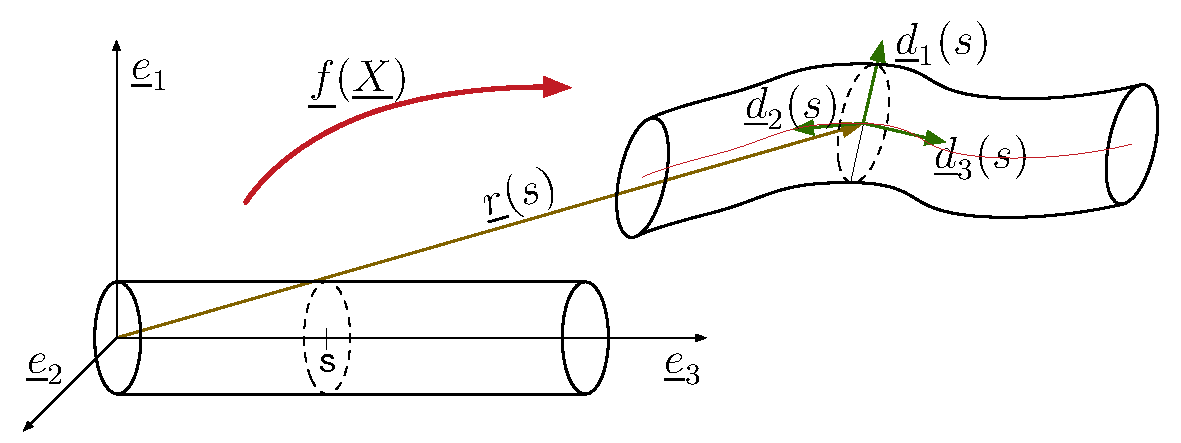
\includegraphics[width=20cm, keepaspectratio=true]{sections/cosserat_rods/images/Kinematics}
  \end{figure}
  
  remember: $s$ is the unique identifier for a particular cross section of the beam
  \vspace{0.6em}
  
  \textbf{kinematic quantities}:
  \begin{itemize}
    \item position of the deformed cross section $\underline{r}(s)$
    \item shearing of the deformed cross section $\underline{d}_1(s)$, $\underline{d}_2(s)$
    \item orientation of the deformed cross section $\underline{d}_3(s)$ \newline
      \null \quad (perpendicular to $\underline{d}_1(s)$ and $\underline{d}_2(s)$ $\rightarrow$ not independent)
    %\item $\doubleunderline{R}(s)$
  \end{itemize}
\end{frame}


%-------------------------------------------------------------------------------
\begin{frame}
  \frametitle{Introduction to \st{special} Cosserat rods (part 2)}

  \textbf{constrained deformation map}
  \begin{displaymath}
    \underline{f}(\underline{X}) = \underline{f}(X_1,X_2,X_3=s) = \underline{r}(s) + X_{\alpha} \, \underline{d}_{\alpha} \quad \text{with } \alpha \in \{1,2\}
  \end{displaymath}
  \vspace{1em}
  
  \textbf{consequences of the imposed kinematic constraints}
  \begin{itemize}
    \item cross sections remain flat
    \item straight lines within the cross section remain straight lines
    \item boundary of the cross section: circles are mapped to ellipses \newline
      \null \quad (not to arbitrary  curves in 2D)
    \item $\underline{d}_1(s)$ and $\underline{d}_2(s)$ are not perpendicular in the general case (shearing)
  \end{itemize}
\end{frame}


%===============================================================================
\subsection{Kinematics of Special Cosserat rods}


%-------------------------------------------------------------------------------
\begin{frame}
  \frametitle{What makes the Special Cosserat rod special?}

  \begin{itemize}
    \item $\underline{d}_1(s)$ and $\underline{d}_2(s)$ \textit{are} perpendicular and unit-normed
    \item hence $\left( \underline{d}_1, \underline{d}_2, \underline{d}_3 \right)$ form an orthonormal triad
  \end{itemize}
  \vspace{1em}
  
  \textbf{consequences}
  \begin{displaymath}
    \exists \: \doubleunderline{R}(s) \in SO(3) \: \forall s : \biggl( R: \left( \underline{e}_1, \underline{e}_2, \underline{e}_3 \right) \mapsto \left( \underline{d}_1, \underline{d}_2, \underline{d}_3 \right) \biggr)
  \end{displaymath}
  \begin{itemize}
    \item $\left( \underline{e}_1, \underline{e}_2, \underline{e}_3 \right)$ is called the global basis
    \item $\left( \underline{d}_1, \underline{d}_2, \underline{d}_3 \right)(s)$ is called the local basis or director basis at $s$
    \item $\underline{d}_i(s) = \doubleunderline{R}(s) \cdot \underline{e}_i$ \quad 
      ($\doubleunderline{R}$ : rotation matrix ; $SO(3)$ : special orthogonal matrix group)
  \end{itemize}
  \vspace{1em}
  
  \textbf{constrained deformation map}
  \begin{displaymath}
    \underline{f}(\underline{X}) = \underline{f}(X_1,X_2,X_3=s) = \underline{r}(s) + \doubleunderline{R}(s) \cdot (X_{\alpha} \, \underline{e}_{\alpha}) \quad \text{with } \alpha \in \{1,2\}
  \end{displaymath}
  
  \vspace{0.5em}
  $\rightarrow$ but the rigidity of the cross section is stiffening the beam!
\end{frame}


%-------------------------------------------------------------------------------
\begin{frame}
  \frametitle{Warp-mode on ;-)}
  
  we want to introduce warping of the cross section, \newline
  while at the same time keeping the director basis $\underline{d}_i$
  \vspace{0.6em}
  
  \textbf{modified deformation map}
  \begin{displaymath}
    \underline{f}(\underline{X}) = \underline{f}(X_1,X_2,X_3=s) = \underline{r}(s) + \doubleunderline{R}(s) \cdot (X_{\alpha} \, \underline{e}_{\alpha} + \underline{u}) \quad \text{with } \alpha \in \{1,2\}
  \end{displaymath}
  
  \vspace{0.3em}
  \textbf{geometric meaning of $\underline{u}$}
  \begin{itemize}
    \item $u_1$, $u_2$ : in-plane shrinking
    \item $u_3$ : out-of-plane warping $\rightarrow$ cross section not planar anymore
    \item then $\underline{d}_1$, $\underline{d}_1$ represent the average orientation of the warped cross section
  \end{itemize}
  \vspace{0.6em}
  
  \textbf{what are our kinematic unknowns?}
  \begin{itemize}
    \item if $\underline{u} = \underline{u}(X_1,X_2,s)$ then we would be dealing with a 3D elasticity problem
    \item here we have $\underline{u}(X_1,X_2,\text{local strains})$, not a function of $s$ \newline (we will come back to this later)
    \item $\underline{r}(s)$ and $\doubleunderline{R}(s)$ are the only kinematic unknowns! (6 scalar quantities)
  \end{itemize}
\end{frame}


%-------------------------------------------------------------------------------
\begin{frame}
  \frametitle{Rotations in 3D revisited}
  
  a \textbf{rotation about \textit{one} axis} is determined by
  \begin{itemize}
    \item axis of rotation given by $\underline{a}$ with $\norm{\underline{a}} = 1$
    \item angle of rotation $\Theta$
  \end{itemize}
  \vspace{0.6em}
  
  \textbf{composition of rotations}
  \begin{displaymath}
    \left( \underline{a}_1, \Theta_1 \right) + \left( \underline{a}_2, \Theta_2 \right) + \left( \underline{a}_3, \Theta_3 \right) + \dots = \left( \underline{a}_{eff}, \Theta_{eff} \right)
  \end{displaymath}
  note: ``$+$'' here denotes the composition of two rotations
  
  \begin{displaymath}
    \doubleunderline{R}_{eff} = \dots \cdot \doubleunderline{R}_3 \cdot \doubleunderline{R}_2 \cdot \doubleunderline{R}_1
  \end{displaymath}
  
  In the general case ($\underline{a}_i \neq \underline{a}_j \text{ for } i \neq j$) rotations do not commute!
  \vspace{1em}
  
  \textbf{example} (rotation about $\underline{e}_3$):
  \begin{displaymath}
    \Biggl( \underline{a} =
    \begin{bmatrix}
      0 \\ 0 \\ 1
    \end{bmatrix}, \Theta \Biggr) \quad \rightarrow \quad
    \doubleunderline{R} =
    \begin{bmatrix}
      +\cos(\Theta) & -\sin(\Theta) & 0 \\
      +\sin(\Theta) & +\cos(\Theta) & 0 \\
      0 & 0 & 1
    \end{bmatrix}
  \end{displaymath}
\end{frame}

%-------------------------------------------------------------------------------
\begin{frame}
  \frametitle{Axis-angle representation of rotations in 3D}
  
  from the axis-angle representation
  \begin{displaymath}
    \Biggl( \underline{a} =
    \begin{bmatrix}
      a_1 \\ a_2 \\ a_3
    \end{bmatrix}, \Theta \Biggr)
  \end{displaymath}
  we obtain the corresponding rotation matrix
  \begin{displaymath}
    \doubleunderline{R} = \exp(\Theta \cdot \doubleunderline{a})  
  \end{displaymath}
  with
  \begin{displaymath}
    \Theta \cdot \doubleunderline{a} = \Theta \cdot 
    \begin{bmatrix}
      0 & -a_3 & a_2 \\
      a_3 & 0 & -a_1 \\
      -a_2 & a_1 & 0
    \end{bmatrix}
  \end{displaymath}
  a skew-symmetric matrix obtained from the definition
  \begin{displaymath}
    \doubleunderline{a} = \doubleunderline{a} \cdot \doubleunderline{I} =
%     \underline{a} \times \doubleunderline{I} :=
    \begin{bmatrix}
      \underline{a} \times \underline{e}_1 & \underline{a} \times \underline{e}_2 & \underline{a} \times \underline{e}_3
    \end{bmatrix}
  \end{displaymath}
  \begin{displaymath}
    \Rightarrow \quad
    \doubleunderline{a} \cdot \underline{v} = \underline{a} \times \underline{v} \quad \forall \underline{v} \in \mathbb{R}^3
  \end{displaymath}
  
  \vspace{0.5em}
  observe the isomorphism between cross products and skew-symmetric matrices:
  \begin{displaymath}
    \underline{a} = \axial(\doubleunderline{a}) = \axial(\underline{a} \times \doubleunderline{I}) = \axial([\underline{a}]_{\times})
  \end{displaymath}
\end{frame}


%-------------------------------------------------------------------------------
\begin{frame}
  \frametitle{Axis-angle representation of rotations in 3D: Rodrigues' formula}
  
  \begin{displaymath}
    \doubleunderline{R} = \cos(\Theta) \, \doubleunderline{I} + \sin(\Theta) \, \doubleunderline{a} + (1-\cos(\Theta)) \, \underline{a} \otimes \underline{a}
  \end{displaymath}
 
  \vspace{1em}
  the Rodrigues' rotation formula allows us to compute the rotation matrix $\doubleunderline{R}$,\newline
  that corresponds to a given axis-angle representation $\left( \underline{a}, \Theta \right)$, \newline
  without actually computing the matrix exponential
  
  \vspace{1em}
  computing matrix exponentials (of non-diagonal matrices) is either expensive or not precise!
  
  \vspace{2em}
  \textbf{example}
  \begin{displaymath}
    \underline{v}_{\text{rotated}} = \doubleunderline{R} \, \underline{v} = \cos(\Theta) \, \underline{v} + \sin(\Theta) \underline{a} \times \underline{v} + (1-\cos(\Theta)) \, (\underline{a} \cdot \underline{v}) \,\underline{a}
  \end{displaymath}
  
%  \begin{displaymath}
%    \doubleunderline{R} = \exp([\underline{a}]_{\times}) = \doubleunderline{I} + \sin(\norm{\underline{a}}) \biggl( \frac{\underline{a}}{\norm{\underline{a}}} \biggr)
%  \end{displaymath}
\end{frame}


%-------------------------------------------------------------------------------
\begin{frame}
  \frametitle{3D rotations expressed by unit quaternions}
  
  Quaternions are a number system that extends the complex numbers. A quaternion consists of one real part and three independent imaginary parts. A unit quaternion is a quaternion of norm one and therefore has three independent components. \newline
  There exists an isomorphism between unit quaternions and rotation matrices:

  \begin{displaymath}
    \text{given }
    \underline{q} = \begin{bmatrix}
      q_0 \\ q_1 \\ q_2 \\ q_3
    \end{bmatrix} \quad \rightarrow \quad
    \doubleunderline{R}(\underline{q}) = 2 \cdot \begin{bmatrix}
      \frac{1}{2} - (q_2^2 + q_3^2) & q_1 \, q_2 - q_0 \, q_3 & q_1 \, q_3 + q_0 \, q_2 \\
      q_1 \, q_2 + q_0 \, q_3 & \frac{1}{2} - (q_1^2 + q_3^2) & q_2 \, q_3 - q_0 \, q_1 \\
      q_1 \, q_3 - q_0 \, q_2 & q_2 \, q_3 + q_0 \, q_1 & \frac{1}{2} - (q_1^2 + q_2^2)
    \end{bmatrix}
  \end{displaymath}
  
  \begin{displaymath}
    \text{real part: } q_0 = \cos \biggl( \frac{\Theta}{2} \biggr) \: \text{ and imaginary part: } \begin{bmatrix}
      q_1 \\ q_2 \\ q_3
    \end{bmatrix} = \sin \biggl( \frac{\Theta}{2} \biggr) \, \underline{a}
  \end{displaymath}
  
  \textbf{advantages}
  \begin{itemize}
    \item quadratic polynomials are faster for computation than $\sin(.)$ and $\cos(.)$
    \item numeric stability: when composing rotations rounding error makes unit quaternions not unit normed but normalizing is simple ; making a slightly non-orthogonal matrix orthogonal again is much harder
  \end{itemize}
\end{frame}


%===============================================================================
\subsection{Balance equations}

%-------------------------------------------------------------------------------
\begin{frame}
  \frametitle{Balance of forces (part 1)}
  % comment about N=+-e_3
  \vspace{-1em}
  \begin{figure}
    \centering
    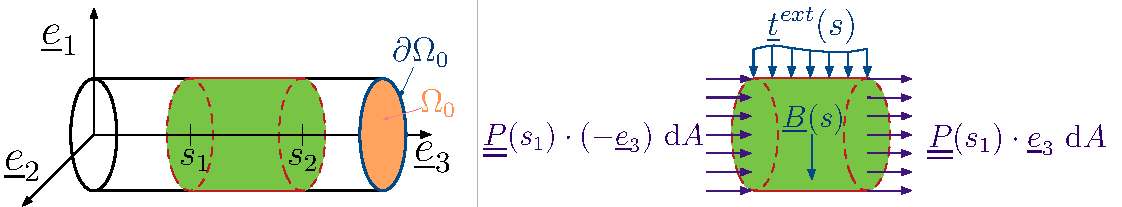
\includegraphics[width=22cm, keepaspectratio=true]{sections/cosserat_rods/images/Forces}
  \end{figure}

  to obtain the forces and moments we integrate the pullback of the tractions / tensions acting in the deformed configuration, hence using the reference configuration as the domain of integration ...
  
  \vspace{1em}
  \textbf{external forces}: body force $\underline{B}$ and external traction $\underline{t}^{ext}$
  \begin{displaymath}
    \begin{alignedat}{1}
      %&\iiint_{\text{undeformed volume}} \underline{B} \dif V + \iint_{\text{lateral surface}} \underline{t}^{ext} \dif A = \\
      %=
      &\int_{s_1}^{s_2} \Biggl( \iint_{\Omega_{0}(s)} \underline{B}(X_1,X_2,s) \dif A + \oint_{\partial \Omega_{0}(s)} \underline{t}^{ext}(l,s) \dif l \Biggr) \dif s =: \\
      =: & \int_{s_1}^{s_2} \underline{\hat{n}}(s) \dif s
    \end{alignedat}
  \end{displaymath}
  \vspace{0.5em}
  $\rightarrow$ distributed external load $\underline{\hat{n}}(s)$ (force per unit of undeformed length)
\end{frame}


%-------------------------------------------------------------------------------
\begin{frame}
  \frametitle{Balance of forces (part 2)}

  %\vspace{-0.5em}
  \begin{figure}
    \centering
    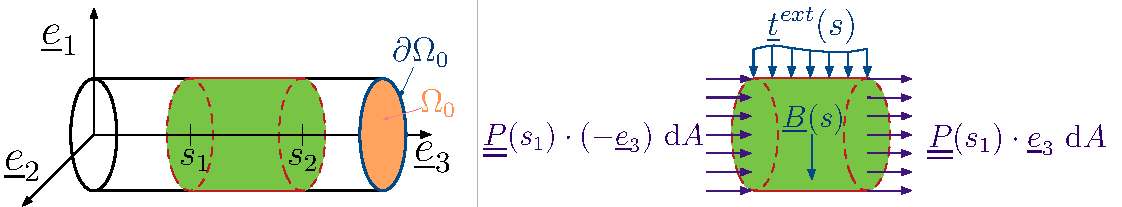
\includegraphics[width=22cm, keepaspectratio=true]{sections/cosserat_rods/images/Forces}
  \end{figure}

  %Material description: $\nabla_{\underline{X}} \cdot \doubleunderline{P} + \underline{B} = \rho_0 \cdot \underline{A}$

  \textbf{internal forces}
  
  \begin{displaymath}
    \begin{alignedat}{1}
      &\iint_{\Omega_0(s)} \doubleunderline{P} \cdot \underline{n} \dif A = \\
      = &\iint_{\Omega_0(s)} \doubleunderline{P}(X_1, X_2, s) \cdot \underline{e}_3 \dif X_1 \dif X_2 = \\
      =: \, &\underline{n}(s)
    \end{alignedat}
  \end{displaymath}
  
  \vspace{0.5em}
  $\rightarrow$ internal contact force $\underline{n}(s)$ (force per unit of undeformed length)
\end{frame}



%-------------------------------------------------------------------------------
\begin{frame}
  \frametitle{Balance of forces (part 3)}
  
  \begin{figure}
    \centering
    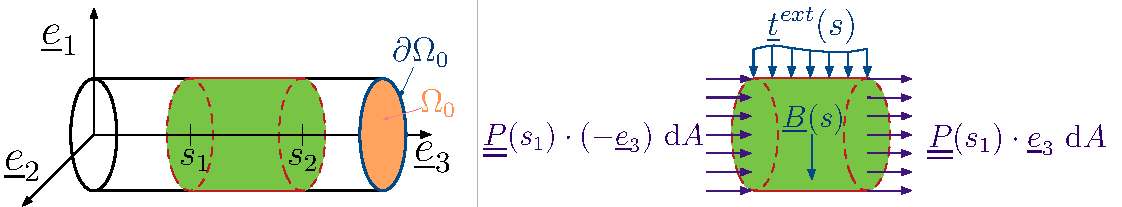
\includegraphics[width=22cm, keepaspectratio=true]{sections/cosserat_rods/images/Forces}
  \end{figure}
  
  \textbf{balance of forces} (statics)
  
  \begin{displaymath}
    \int_{s_1}^{s_2} \underline{\hat{n}}(s) \dif s + \underline{n}(s_2) - \underline{n}(s_1) =
    \int_{s_1}^{s_2} \underline{\hat{n}}(s) + \underline{n}^{\prime}(s) \dif s =
    \underline{0}
  \end{displaymath}
  
  since $s_1$ and $s_2$ are arbitrary cross sections we let $s_2 \to s_1$ \newline
  and obtain the \textbf{local force balance}
  \begin{displaymath}
    \underline{n}^{\prime}(s) + \underline{\hat{n}}(s) = \underline{0}
  \end{displaymath}
  \vspace{0.6em}
  
  \textbf{local balance of linear momentum} (dynamics)
  \begin{displaymath}
    \underline{n}^{\prime}(s) + \underline{\hat{n}}(s) = \rho_0 \cdot A \cdot \underline{\ddot{r}}(s)
  \end{displaymath}
\end{frame}


%-------------------------------------------------------------------------------
\begin{frame}
  \frametitle{Balance of moments (part 1)}
  
  we write the moment balance about the origin: $\underline{M} = \underline{x} \times \underline{F}$ \newline
  with $\underline{x}(X_1,X_2,s) = \underline{r}(s) + \bigl( \underline{x}(X_1,X_2,s) - \underline{r}(s) \bigr)$
  \vspace{0.5em}
  
  \textbf{moment due to external loads}
  \begin{displaymath}
    \begin{alignedat}{1}
      &\iiint_{\text{reference volume}} \underline{x} \times \underline{B} \dif V +
      \iint_{\text{lateral surface of reference volume}} \underline{x} \times \underline{t}^{ext} \dif A = \\ 
      = &{\color{faublue} \int_{s_1}^{s_2} \Biggl( \underline{r}(s) \times \iint_{\Omega_{0}(s)} \underline{B}(X_1,X_2,s) \dif A \Biggr) \dif s } + \\
      + &{\color{og_dark_green} \int_{s_1}^{s_2} \Biggl( \iint_{\Omega_{0}(s)} \bigl( \underline{x}(X_1,X_2,s) - \underline{r}(s) \bigr) \times \underline{B}(X_1,X_2,s) \dif A \Biggr) \dif s } + \\
      + &{\color{faublue} \int_{s_1}^{s_2} \Biggl( \underline{r}(s) \times \oint_{\partial \Omega_{0}(s)} \underline{t}^{ext}(l,s) \dif l \Biggr) \dif s } + \\
      + &{\color{og_dark_green} \int_{s_1}^{s_2} \Biggl( \oint_{\partial \Omega_{0}(s)} \bigl( \underline{x}(X_1,X_2,s) - \underline{r}(s) \bigr) \times \underline{t}^{ext}(l,s) \dif l \Biggr) \dif s } =
    \end{alignedat}
  \end{displaymath}
\end{frame}



%-----------------------------0108897834-------------------------------------------------
\begin{frame}
  \frametitle{Balance of moments (part 2)}
  \begin{displaymath}
    \begin{alignedat}{1}
      = &{\color{faublue} \int_{s_1}^{s_2} \Biggl( \underline{r}(s) \times \biggl( \iint_{\Omega_0} \underline{B}(X_1,X_2,s) \dif A + \oint_{\partial \Omega_{0}(s)} \underline{t}^{ext}(s) \dif l \biggr) \Biggr) \dif s} + \\
        + &{\color{og_dark_green} \int_{s_1}^{s_2} \biggl( \iint_{\Omega_{0}(s)} \bigl( \underline{x}(X_1,X_2,s) - \underline{r}(s) \bigr) \times \underline{B}(X_1,X_2,s) \dif A + } \\
        &{\color{og_dark_green} \quad \: \, + \oint_{\partial \Omega_0} \bigl( \underline{x}(X_1,X_2,s) - \underline{r}(s) \bigr) \times \underline{t}^{ext}(l,s) \dif l \biggr) \dif s } = \\
      =: &{\color{faublue} \int_{s_1}^{s_2} \underline{r}(s) \times \underline{\hat{n}}(s) \dif s} +
        {\color{og_dark_green} \int_{s_1}^{s_2} \underline{\hat{m}}(s) \dif s}
    \end{alignedat}
  \end{displaymath}
\end{frame}


%-------------------------------------------------------------------------------
\begin{frame}
  \frametitle{Balance of moments (part 3)}
  \textbf{moment due to internal forces}
  \begin{displaymath}
    \begin{alignedat}{1}
      &\iint_{\Omega_0(s)} \underline{x}(X_1,X_2,s) \times \bigl( \doubleunderline{P}(X_1,X_2,s) \cdot \underline{e}_3 \bigr) \dif A = \\
      =&{\color{faublue} \iint_{\Omega_0(s)} \underline{r}(s) \times \bigl( \doubleunderline{P}(X_1,X_2,s) \cdot \underline{e}_3 \bigr) \dif X_1 \dif X_2} + \\
      + &{\color{og_dark_green} \iint_{\Omega_0(s)} \bigl( \underline{x}(X_1,X_2,s) - \underline{r}(s) \bigr) \times \bigl( \doubleunderline{P}(X_1,X_2,s) \cdot \underline{e}_3 \bigr) \dif X_1 \dif X_2} = \\
      = \, &{\color{faublue} \underline{r}(s) \times \iint_{\Omega_0(s)} \doubleunderline{P}(X_1,X_2,s) \cdot \underline{e}_3 \dif X_1 \dif X_2} + {\color{og_dark_green} \dots} = \\
      =: \, &{\color{faublue} \underline{r}(s) \times \underline{n}(s)} +
        {\color{og_dark_green} \underline{m}(s)}
    \end{alignedat}
  \end{displaymath}
\end{frame}


%-------------------------------------------------------------------------------
\begin{frame}
  \frametitle{Balance of moments (part 4)}
  
  \textbf{balance of moments} (statics)
  \begin{displaymath}
    \begin{alignedat}{1}
      &\int_{s_1}^{s_2} \bigl( \underline{r}(s) \times \underline{\hat{n}}(s) + \underline{\hat{m}}(s)\bigr) \dif s + \\ 
      &+ \bigl( \underline{r}(s_2) \times \underline{n}(s_2) + \underline{m}(s_2) \bigr)
         - \bigl( \underline{r}(s_1) \times \underline{n}(s_1) + \underline{m}(s_1) \bigr) = \\
      &= \int_{s_1}^{s_2} \Bigl( \bigl( \cancel{\underline{r}(s) \times \underline{\hat{n}}(s)} + \underline{\hat{m}}(s) \bigr) + \bigl( \underline{r}^{\prime}(s) \times \underline{n}(s) + \cancel{\underline{r}(s) \times \underline{n}^{\prime}(s)} + \underline{m}^{\prime}(s) \bigr) \Bigr) \dif s = \\
      &= \int_{s_1}^{s_2} \bigl( \underline{\hat{m}}(s) + \underline{r}^{\prime}(s) \times \underline{n}(s) + \underline{m}^{\prime}(s) \bigr) \dif s
    \end{alignedat}
  \end{displaymath}
  % Note: terms canceled because of force balance
  
  since $s_1$ and $s_2$ are arbitrary cross sections we let $s_2 \to s_1$ \newline
  and obtain the \textbf{local moment balance}
  \begin{displaymath}
    \underline{m}^{\prime}(s) + \underline{r}^{\prime}(s) \times \underline{n}(s) + \underline{\hat{m}}(s) = \underline{0}
  \end{displaymath}

  \vspace{0.7em}
  \textbf{local balance of angular momentum} (dynamics) (with $\doubleunderline{I}_0$ the moment of area tensor)
  \begin{displaymath}
    \underline{m}^{\prime}(s) +
    \underline{r}^{\prime}(s) \times \underline{n}(s) +
    \underline{\hat{m}}(s) =
    \rho_0 \cdot
    \od{}{t} \bigl( \doubleunderline{I}_0 \cdot \underline{\omega} \bigr)
  \end{displaymath}
\end{frame}


%-------------------------------------------------------------------------------

\begin{frame}
  \frametitle{Review of balance equations (statics)}
  
  \textbf{force balance} (3 equations)
  \begin{displaymath}
    \underline{n}^{\prime}(s) + \underline{\hat{n}}(s) = \underline{0}
  \end{displaymath}
  
  \textbf{moment balance} (3 equations)
  \begin{displaymath}
    \underline{m}^{\prime}(s) + \underline{r}^{\prime}(s) \times \underline{n}(s) + \underline{\hat{m}}(s) = \underline{0}
  \end{displaymath}
  
  \vspace{1em}
  we have \textbf{6 kinematic unknowns}, $\underline{r}(s)$ and $\doubleunderline{R}(s)$ with 3 unknowns each,
  
  \vspace{0.3em}
  and we have \textbf{6 kinetic unknowns}
  \begin{displaymath}
    \begin{alignedat}{1}
      &\underline{n}(s) = \iint_{\Omega_0(s)} \doubleunderline{P}(X_1, X_2, s) \cdot \underline{e}_3 \dif X_1 \dif X_2 \\
      &\underline{m}(s) = \iint_{\Omega_0(s)} \bigl( \underline{x}(X_1,X_2,s) - \underline{r}(s) \bigr) \times \bigl( \doubleunderline{P}(X_1,X_2,s) \cdot \underline{e}_3 \bigr) \dif X_1 \dif X_2
    \end{alignedat}
  \end{displaymath}
  
  \vspace{0.3em}
  to close the system, we need a relationship between the kinematic and the kinetic quantities
  
  \vspace{0.2em}
  $\rightarrow$ this relationship is called \textit{constitutive law of the material}
\end{frame}


%===============================================================================
\subsection{Constitutive laws}

%-------------------------------------------------------------------------------
\begin{frame}
  \frametitle{Motivation of constitutive law}

  let's recall the \textbf{constrained deformation map} (without warping)
  \begin{displaymath}
    \underline{x}(X_1,X_2,s) = \underline{f}(X_1,X_2,s) = \underline{r}(s) + X_{\alpha} \, \underline{d}_{\alpha} = \underline{r}(s) + \doubleunderline{R}(s) \cdot ( X_{\alpha} \, \underline{e}_{\alpha} )
  \end{displaymath}
  
  we compute the \textbf{deformation gradient} and obtain
  % TODO ?computation of F in more detail?
  \begin{displaymath}
    \begin{alignedat}{1}
      \doubleunderline{F}(X_1,X_2,s) &= \underline{r}^{\prime}(s) \otimes \underline{e}_3 + \doubleunderline{R}(s) \cdot \bigl( \underline{e}_{\alpha} \otimes \underline{e}_{\alpha} \bigr) + \doubleunderline{R}^{\prime}(s) \cdot \bigl( X_{\alpha} \underline{e}_{\alpha} \bigr) \otimes \underline{e}_3 = \\
      &= \doubleunderline{R}(s) \cdot \biggl( \doubleunderline{R}^{\mathrm{T}}(s) \cdot \underline{r}^{\prime}(s) \otimes \underline{e}_3 + \underline{e}_{\alpha} \otimes \underline{e}_{\alpha} + \doubleunderline{R}^{\mathrm{T}}(s) \cdot \doubleunderline{R}^{\prime}(s) \cdot \bigl( X_{\alpha} \underline{e}_{\alpha} \bigr) \otimes \underline{e}_3 \biggr)
    \end{alignedat}
  \end{displaymath}
  
  \vspace{1em}
  we then obtain an expression of the form
  \begin{displaymath}
    \doubleunderline{P}(X_1,X_2,s) = \mathop{\mathrm{function}}\bigl( \doubleunderline{F}(X_1,X_2,s) \bigr) \, ,
  \end{displaymath}
  
  \vspace{0.4em}
  from the 3-dimensional constitutive law of the material
\end{frame}



%-------------------------------------------------------------------------------
\begin{frame}
  \frametitle{Example with constrained deformation map: stretching of a bar}
  
  \vspace{-1em}
  \begin{multicols}{2}
    \noindent
    \begin{figure}
      \centering
      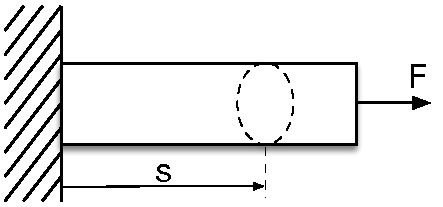
\includegraphics[width=8cm, keepaspectratio=true]{sections/cosserat_rods/images/ExampleConstrainedMapStretchingBar}
    \end{figure}
    
    we have the \textbf{deformed configuration}
    \begin{displaymath}
      \begin{alignedat}{1}
        \underline{r}(s) &= \lambda \, s \, \underline{e}_3 \quad \text{with } \lambda \in \mathbb{R}^{+} \\
        \doubleunderline{R}(s) &= \doubleunderline{I} \\
      \end{alignedat}
    \end{displaymath}
  \end{multicols}
  
  \vspace{-0.5em}
  therefore the \textbf{deformation map} is
  \begin{displaymath}
    \underline{x}(X_1,X_2,s) \underline{x}(s) = \lambda \, s \, \underline{e}_3 + \doubleunderline{I} \cdot (X_{\alpha} \, \underline{e}_{\alpha})
  \end{displaymath}
  
  and its \textbf{deformation gradient} is given by
  \begin{displaymath}
    \doubleunderline{F}(X_1,X_2,s) = \doubleunderline{F}(s) = \lambda \, \underline{e_3} \otimes \underline{e_3} + \underline{e}_{\alpha} \otimes \underline{e}_{\alpha} = (\lambda - 1) \underline{e}_3 \otimes \underline{e}_3 + \doubleunderline{I}  
  \end{displaymath}
  
  but the \textbf{axial force}
  \begin{displaymath}
    \begin{alignedat}{1}
      \underline{n}(s) &= \iint_{\Omega_0(s)} \doubleunderline{P}(X_1, X_2, s) \cdot \underline{e}_3 \dif X_1 \dif X_2 \\
      &\neq E \, A \, (\lambda - 1)
    \end{alignedat}
  \end{displaymath}
  because the deformation map violates the traction-free boundary condition \newline
  $\rightarrow$ the cross section must be able to shrink when the bar is stretched!
\end{frame}


%-------------------------------------------------------------------------------
\begin{frame}
  \frametitle{Constitutive equation for a hyperelastic rod}

  \begin{itemize}
    \item a hyperelastic material is a model for reversible elasticity $\rightarrow$ stress-strain relationship derives from a potential function, i.e. the strain energy density of the material
    \item in general a hyperelastic material has a nonlinear stress-strain relationship
    \item well known hyperelastic material models are the Neo-Hookean and Mooney-Rivlin solids
  \end{itemize}
  
  \vspace{1.5em}
  \textbf{strain energy per unit of undeformed length}
  \begin{displaymath}
    \phi = \phi \bigl( \underline{r}(s),\doubleunderline{R}(s),\underline{r}^{\prime}(s),\doubleunderline{R}^{\prime}(s) \bigr)
  \end{displaymath}
  
  \vspace{1.5em}
  \textbf{strain energy per unit of undeformed volume}
  \begin{displaymath}
    W \bigl( \cancel{\underline{f}(s)}, \doubleunderline{F}(s), \cancel{\nabla \doubleunderline{F}(s)} \bigr) = W \bigl( \doubleunderline{F}(s) \bigr)
  \end{displaymath}

  \vspace{0.1em}
  \begin{itemize}
    \item $\underline{f}(s)$ canceled because of principle of frame-indifference
    \item $\nabla \doubleunderline{F}(s)$ canceled because we will not consider higher order derivatives of the deformation map in classical elasticity (compared to higher gradient elasticity theory)
    % higher gradient elasticity: when there exist discontinuities at interfaces in the material 
  \end{itemize}
\end{frame}


%-------------------------------------------------------------------------------
\begin{frame}
  \frametitle{Principle of material frame-indifference (part 1)}

  \vspace{-0.5em}
  \begin{itemize}
    \item  constitutive laws should be invariant with regard to the external frame of reference, \newline i.e. the coordinate system ($\rightarrow$ observer objectivity)
    \item $\Rightarrow$ rigid body motions do not affect the internally stored energy in the system, \newline \null \quad (i.e. the mechanical/deformation energy)
    \item $\rightarrow$ we want to identify a set of strain measures which is invariant to rigid body motions!
  \end{itemize}
  
  \vspace{0.3em}
  to that end we set up a simple \textbf{thought experiment}
  \begin{itemize}
    \item perform two rigid body motions: one rotation followed by one translation
    \item equate the internal mechanical energy potentials: $\eval[1]{\phi}_{\alpha} = \eval[1]{\phi}_{\beta} = \eval[1]{\phi}_{\gamma}$
  \end{itemize}
  
  \vspace{-1.4em}
  \begin{figure}
    \centering
    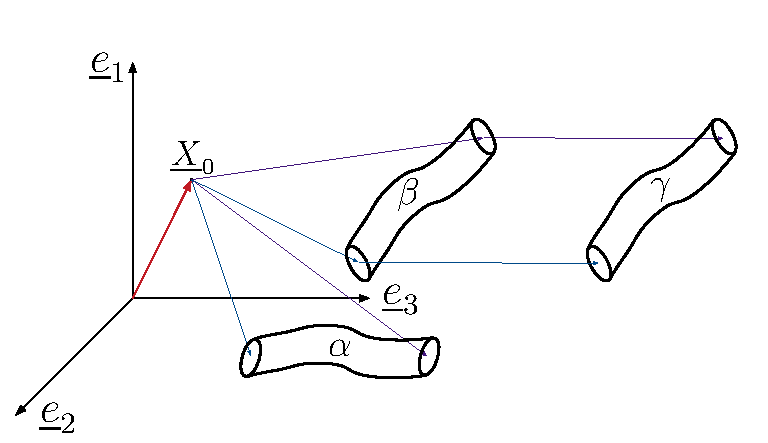
\includegraphics[width=13cm, keepaspectratio=true]{sections/cosserat_rods/images/FrameIndifferenceExperiment}
  \end{figure}  
\end{frame}


%-------------------------------------------------------------------------------
\begin{frame}
  \frametitle{Principle of material frame-indifference (part 2)}
  \vspace{-0.6em}
  \begin{enumerate}
    \item initial configuration $\alpha$
      \begin{itemize}
        \item centerline given by $\underline{r}^{\alpha}(s)$
        \item cross section orientation given by $\doubleunderline{R}^{\alpha}(s)$
        \item energy potential given by $\eval[1]{\phi}_{\beta}(s) = \phi \bigl( \underline{r}^{\alpha}{\alpha}(s) , \, \doubleunderline{R}^{\alpha}(s) , \, \underline{r}^{\alpha \prime}(s) , \, \doubleunderline{R}^{\alpha \prime}(s) \bigr)$
      \end{itemize}
      
    \item configuration $\beta$ after rigid body rotation by some $\doubleunderline{Q} \in SO(3)$ about some $\underline{X}_0 \in \mathbb{R}^3$
      \begin{itemize}
        \item $\underline{r}^{\beta}(s) = \underline{X}_0 + \doubleunderline{Q} \left( \underline{r}^{\alpha}(s) - \underline{X}_0 \right) \quad \Rightarrow \quad \underline{r}^{\beta \prime}(s) = \doubleunderline{Q} \, \underline{r}^{\alpha \prime}(s)$ \newline
          \null \quad (shift coordinate system s.t. rotation's fix-point $\hat{=}$ origin; rotate; undo shift)
        \item $\doubleunderline{R}^{\beta}(s) = \doubleunderline{Q} \, \doubleunderline{R}^{\alpha}(s) \quad \Rightarrow \quad \doubleunderline{R}^{\beta \prime}(s) = \doubleunderline{Q} \, \doubleunderline{R}^{\alpha \prime}(s)$
        \item $\eval[1]{\phi}_{\beta}(s) = \phi \bigl( \underline{X}_0 + \doubleunderline{Q} \left( \underline{r}^{\alpha}(s) - \underline{X}_0 \right) , \, \doubleunderline{Q} \, \doubleunderline{R}^{\alpha}(s) , \, \doubleunderline{Q} \, \underline{r}^{\alpha \prime}(s) , \, \doubleunderline{Q} \, \doubleunderline{R}^{\alpha \prime}(s) \bigr)$
      \end{itemize}
      
    \item configuration $\gamma$ after rigid body translation by some $\underline{t} \in \mathbb{R}^3$
      \begin{itemize}
        \item $\underline{r}^{\gamma}(s) = \underline{X}_0 + \doubleunderline{Q} \left( \underline{r}^{\alpha}(s) - \underline{X}_0 \right) + \underline{t} \quad \Rightarrow \quad \underline{r}^{\gamma \prime}(s) = \underline{r}^{\beta \prime}(s) = \doubleunderline{Q} \,\underline{r}^{\alpha \prime}(s)$
        \item $\doubleunderline{R}^{\gamma}(s) = \doubleunderline{I} \, \doubleunderline{R}^{\beta}(s) = \doubleunderline{Q} \, \doubleunderline{R}^{\alpha}(s) \quad \Rightarrow \quad \doubleunderline{R}^{\gamma \prime}(s) = \doubleunderline{R}^{\beta \prime}(s) = \doubleunderline{Q} \, \doubleunderline{R}^{\alpha \prime}(s)$
        \item $\eval[1]{\phi}_{\gamma}(s) = \phi \bigl( \underline{X}_0 + \doubleunderline{Q} \left( \underline{r}^{\alpha}(s) - \underline{X}_0 \right) + \underline{t} , \, \doubleunderline{Q} \, \doubleunderline{R}^{\alpha}(s) , \, \doubleunderline{Q} \,\underline{r}^{\alpha \prime}(s) , \, \doubleunderline{Q} \, \doubleunderline{R}^{\alpha \prime}(s) \bigr)$
      \end{itemize}
  \end{enumerate}
\end{frame}



%-------------------------------------------------------------------------------
\begin{frame}
  \frametitle{Principle of material frame-indifference (part 3)}
  
  comparing $\eval[1]{\phi}_{\beta}(s) \overset{!}{=} \eval[1]{\phi}_{\gamma}(s)$ gives
  \begin{displaymath}
    \begin{alignedat}{4}
      \phi \bigl(
        &\underline{X}_0 + \doubleunderline{Q} \left( \underline{r}^{\alpha}(s) - \underline{X}_0 \right) , \,
        &\doubleunderline{Q} \, \doubleunderline{R}^{\alpha}(s) , \,
        &\doubleunderline{Q} \, \underline{r}^{\alpha \prime}(s) , \,
        &\doubleunderline{Q} \, \doubleunderline{R}^{\alpha \prime}(s)
      \bigr) = \\
      \phi \bigl(
        &\underline{X}_0 + \doubleunderline{Q} \left( \underline{r}^{\alpha}(s) - \underline{X}_0 \right) + \underline{t} , \,
        &\doubleunderline{Q} \, \doubleunderline{R}^{\alpha}(s) , \,
        &\doubleunderline{Q} \, \underline{r}^{\alpha \prime}(s) , \,
        &\doubleunderline{Q} \, \doubleunderline{R}^{\alpha \prime}(s)
      \bigr) \Rightarrow
    \end{alignedat}
  \end{displaymath}
  $\Rightarrow \phi$ is independent of $\underline{r}(s)$, i.e. the first argument can be omitted
  
  \vspace{1em}
  without loss of generality we can set the arbitrarily chosen rotation matrix $\doubleunderline{Q} := \doubleunderline{R}^{\mathrm{T}}$
  \begin{displaymath}
    \phi(s) = \phi \bigl(
        . , \,
        \doubleunderline{R}^{\mathrm{T}}(s) \, \doubleunderline{R}(s) , \,
        \doubleunderline{R}^{\mathrm{T}}(s) \, \underline{r}^{\prime}(s) , \,
        \doubleunderline{R}^{\mathrm{T}}(s) \, \doubleunderline{R}^{\prime}(s)
      \bigr)
  \end{displaymath}
  
  \vspace{1em}
  we define a new version of $\phi$ that depends only on the invariants
  \begin{displaymath}
    \psi(s) := \psi \bigl(
      \doubleunderline{R}^{\mathrm{T}}(s) \, \underline{r}^{\prime}(s) , \,
      \doubleunderline{R}^{\mathrm{T}}(s) \, \doubleunderline{R}^{\prime}(s)
    \bigr)
  \end{displaymath}  
\end{frame}


%-------------------------------------------------------------------------------
\begin{frame}
  \frametitle{Invariant strain measures (part 1)}
  
  
  we can verify that $\doubleunderline{R}^{\mathrm{T}} \, \underline{r}^{\prime}$ and $\doubleunderline{R}^{\mathrm{T}} \, \doubleunderline{R}^{\prime}$ are truly invariant strain measures:
  
  \vspace{1em}
  we get
  \begin{displaymath}
    \doubleunderline{R}^{\gamma \mathrm{T}} \, \underline{r}^{\gamma \prime} =
    \bigl( \doubleunderline{Q} \, \doubleunderline{R}^{\alpha} \bigr)^{\mathrm{T}} \, \bigl( \doubleunderline{Q} \, \underline{r}^{\alpha \prime} \bigr) =
    \bigl( \doubleunderline{R}^{\alpha \mathrm{T}} \, \doubleunderline{Q}^{\mathrm{T}} \bigr) \, \bigl( \doubleunderline{Q} \, \underline{r}^{\alpha \prime} \bigr) =
    \doubleunderline{R}^{\alpha \mathrm{T}} \, \underline{r}^{\alpha \prime}
  \end{displaymath}
  and
  \begin{displaymath}
    \doubleunderline{R}^{\gamma \mathrm{T}} \, \doubleunderline{R}^{\gamma \prime} =
    \bigl( \doubleunderline{Q} \, \doubleunderline{R}^{\alpha} \bigr)^{\mathrm{T}} \, \bigl( \doubleunderline{Q} \, \doubleunderline{R}^{\alpha \prime} \bigr) =
    \bigl( \doubleunderline{R}^{\alpha \mathrm{T}} \, \doubleunderline{Q}^{\mathrm{T}} \bigr) \, \bigl( \doubleunderline{Q} \, \doubleunderline{R}^{\alpha \prime} \bigr) =
    \doubleunderline{R}^{\alpha \mathrm{T}} \, \doubleunderline{R}^{\alpha \prime}
  \end{displaymath}
\end{frame}


%-------------------------------------------------------------------------------
\begin{frame}
  \frametitle{Invariant strain measures (part 2)}
  we define $\underline{v}$ as the shorthand for the first invariant
  \begin{displaymath}
    \underline{v} =
    \begin{bmatrix} v_1 \\ v_2 \\ v_3 \end{bmatrix} = 
    v_i \, \underline{e}_i :=
    \doubleunderline{R}^{\mathrm{T}} \, \underline{r}^{\prime}
    \quad \Rightarrow \quad
    \underline{r}^{\prime} =
    \doubleunderline{R} \, \underline{v} =
    v_i \, \doubleunderline{R} \, \underline{e}_i =
    v_i \, \underline{d}_i
  \end{displaymath}
  
  and from orthogonality of the director basis ($\underline{d}_i \cdot \underline{d}_j = \delta_{ij}$) it follows that $v_i = \underline{r}^{\prime} \cdot \underline{d}_i$
  
  \vspace{0.3em}
  $\rightarrow \underline{v} = \doubleunderline{R}^{\mathrm{T}} \, \underline{r}^{\prime}$ is the centerline tangent vector resolved in the local director basis!
  
  \vspace{1em}
  more specifically we have ...
  \begin{itemize}
    \item $v_1 = \underline{r}^{\prime} \, \underline{d}_1$ : rate of transverse shift $\hat{=}$ shear along $\underline{d}_1$
    \item $v_2 = \underline{r}^{\prime} \, \underline{d}_2$ : shear along $\underline{d}_2$
    \item $v_3 = \underline{r}^{\prime} \, \underline{d}_3$ : rate of axial shift $\hat{=}$ axial stretch 
  \end{itemize}
  % TODO ?make a figure
\end{frame}


%-------------------------------------------------------------------------------
\begin{frame}
  \frametitle{Invariant strain measures (part 3)}
  
  we define $\doubleunderline{K}$ as the shorthand for the second invariant
  \begin{displaymath}
    \doubleunderline{K} =
    K_{ij} \, \underline{e}_i \otimes \underline{e}_j :=
    \doubleunderline{R}^{\mathrm{T}} \, \doubleunderline{R}^{\prime}
  \end{displaymath}
  
  \vspace{0.5em}
  \textbf{proof} that $\doubleunderline{K}$ is \textit{skew-symmetric} ($K_{ij} = -K_{ji}$)
  \begin{displaymath}
    \doubleunderline{R}^{\mathrm{T}} \, \doubleunderline{R} = \doubleunderline{I}
    \quad \Rightarrow \quad
    \doubleunderline{R}^{\mathrm{T}} \, \doubleunderline{R}^{\prime} + \doubleunderline{R}^{\prime \mathrm{T}} \, \doubleunderline{R} = \doubleunderline{0}
    \quad \Rightarrow \quad
    \doubleunderline{K} = -\doubleunderline{K}^{\mathrm{T}}
  \end{displaymath}
  
  \vspace{0.5em}
  we therefore can write
  \begin{displaymath}
    \doubleunderline{K} = 
    \begin{bmatrix}
       0   & -k_3 &  k_2 \\
       k_3 &  0   & -k_1 \\
      -k_2 &  k_1 &  0
    \end{bmatrix}
  \end{displaymath}
  \vspace{0.5em}
  and we recall that $\doubleunderline{K} \, \underline{a} = \underline{k} \times \underline{a} \: \forall \underline{a} \in \mathbb{R}^3$ with $\underline{k} = \axial(\doubleunderline{K}) = k_i \, \underline{e}_i$
  
  \vspace{1em}
  $\rightarrow$ with $\left( \underline{v} , \, \underline{k} \right)$ we have the 6 strain measures given in the frame of the director basis! \newline
  $\rightarrow$ $\psi = \psi \bigl( \underline{v} , \, \doubleunderline{K} \bigr) =: \hat{\psi} \bigl( \underline{v} , \, \underline{k} \bigr)$ (for easy notation we will drop the $\hat{.}$ in the sequel)
\end{frame}


%-------------------------------------------------------------------------------
\begin{frame}
  \frametitle{Invariant strain measures (part 4)}

  to better understand the physical meaning of $\underline{k}$ we have a look at two examples ...
  
  \vspace{0.5em}
  \textbf{pure twisting of a rod}
  \vspace{-1em}
  \begin{multicols}{2}
    \noindent
    
    \begin{figure}
      \centering
      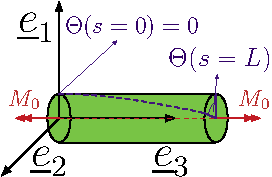
\includegraphics[width=10cm, keepaspectratio=true]{sections/cosserat_rods/images/PureTwistingExample}
    \end{figure}

    \begin{itemize}
      \item rotation of cross sections around $\underline{e}_3$-axis
      \item angle of rotation for the cross section at $s$ given by $\Theta(s) = \Theta^{\prime} \cdot s$ \newline
        with $\Theta^{\prime} = const.$ because external moments act only at $s=0$ and $s=L$
    \end{itemize}
    \vspace{0.1em}
    \begin{displaymath}
      \underline{r}(s) = s \cdot \underline{e}_3 
      \: \Rightarrow \:
      \underline{r}^{\prime}(s) = \underline{e}_3
    \end{displaymath}
    \begin{displaymath}
      \: \Rightarrow \:
      \underline{v} = \doubleunderline{R}^{\mathrm{T}} \, \underline{r}^{\prime} =
      \begin{bmatrix}
        0 & 0 & 1
      \end{bmatrix}^{\mathrm{T}}
      \: \Rightarrow \:
      v_3 = 1
    \end{displaymath}
%    \begin{displaymath}
%      \underline{r}(s) = s \cdot \underline{e}_3 
%      \: \Rightarrow \:
%      \underline{r}^{\prime}(s) = \underline{e}_3
%      \: \Rightarrow \:
%      \underline{v} = \doubleunderline{R}^{\mathrm{T}} \, \underline{r}^{\prime} =
%      \begin{bmatrix}
%        0 & 0 & 1
%      \end{bmatrix}^{\mathrm{T}}
%      \: \Rightarrow \:
%      v_3 = 1
%    \end{displaymath}
  \end{multicols}
  \vspace{-1.2em}
  \begin{displaymath}
    \doubleunderline{R}(s) =
    \begin{bmatrix}
      +\cos(\Theta(s)) & -\sin(\Theta(s)) & 0 \\
      +\sin(\Theta(s)) & +\cos(\Theta(s)) & 0 \\
      0 & 0 & 1
    \end{bmatrix}
    \: \Rightarrow \:
    \doubleunderline{R}^{\prime}(s) =
    \Theta^{\prime} \cdot
    \begin{bmatrix}
      -\sin(\Theta(s)) & -\cos(\Theta(s)) & 0 \\
      +\cos(\Theta(s)) & -\sin(\Theta(s)) & 0 \\
      0 & 0 & 0
    \end{bmatrix}
  \end{displaymath}
    
  \begin{displaymath}
    \doubleunderline{K}(s) =
    \doubleunderline{R}^{\mathrm{T}}(s) \, \doubleunderline{R}^{\prime}(s) =
    \begin{bmatrix}
      0 & -\Theta^{\prime} & 0 \\
      +\Theta^{\prime} & 0 & 0 \\
      0 & 0 & 0
    \end{bmatrix}
    \: \Rightarrow \:
    \underline{k} =
    \begin{bmatrix}
      0 \\ 0 \\ \Theta^{\prime}
    \end{bmatrix}
    \: \Rightarrow \:
    k_3 = \Theta^{\prime}
  \end{displaymath}
\end{frame}

%-------------------------------------------------------------------------------
\begin{frame}
  \frametitle{Invariant strain measures (part 5)}

  \textbf{pure bending of a rod}
  \begin{multicols}{2}
    \noindent
    \begin{figure}
      \centering
      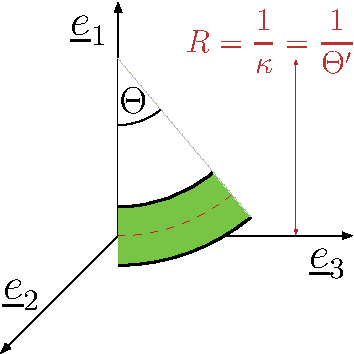
\includegraphics[width=8cm, keepaspectratio=true]{sections/cosserat_rods/images/PureBendingExample}
    \end{figure}
    
    \begin{itemize}
      \item rotation of cross sections around $\underline{e}_2$-axis
      \item angle of rotation for the cross section at $s$ given by $\Theta(s) = \Theta^{\prime} \cdot s = \kappa \cdot s$\newline
        with $\Theta^{\prime} = \kappa = const.$ because external moments act only at $s=0$ and $s=L$
    \end{itemize}
    \vspace{0.1em}
    \begin{displaymath}
      \underline{r}(s) = s \cdot \underline{e}_3 
      \: \Rightarrow \:
      \underline{r}^{\prime}(s) = \underline{e}_3
    \end{displaymath}
    \begin{displaymath}
      \: \Rightarrow \:
      \underline{v} = \doubleunderline{R}^{\mathrm{T}} \, \underline{r}^{\prime} =
      \begin{bmatrix}
        0 & 0 & 1
      \end{bmatrix}^{\mathrm{T}}
      \: \Rightarrow \:
      v_3 = 1
    \end{displaymath}
    \vspace{0.6em}
  \end{multicols}  

  \vspace{-2em}
  \begin{displaymath}
    \doubleunderline{R}(s) =
    \begin{bmatrix}
      +\cos(\Theta(s)) & 0 & +\sin(\Theta(s))\\
      0 & 1 & 0 \\
      -\sin(\Theta(s)) & 0 & +\cos(\Theta(s))
    \end{bmatrix}
    \: \Rightarrow \:
    \doubleunderline{R}^{\prime}(s) =
    \Theta^{\prime} \cdot
    \begin{bmatrix}
      -\sin(\Theta(s)) & 0 & +\cos(\Theta(s))\\
      0 & 0 & 0 \\
      -\cos(\Theta(s)) & 0 & -\sin(\Theta(s))
    \end{bmatrix}
  \end{displaymath}
  
  \begin{displaymath}
    \doubleunderline{K}(s) =
    \doubleunderline{R}^{\mathrm{T}}(s) \, \doubleunderline{R}^{\prime}(s) =
    \begin{bmatrix}
      0 & 0 & +\Theta^{\prime} \\
      0 & 0 & 0 \\
      -\Theta^{\prime} & 0 & 0
    \end{bmatrix}
    \: \Rightarrow \:
    \underline{k} =
    \begin{bmatrix}
      0 \\ \Theta^{\prime} \\ 0
    \end{bmatrix}
    \: \Rightarrow \:
    k_2 = \Theta^{\prime}
  \end{displaymath}
\end{frame}

%-------------------------------------------------------------------------------
\begin{frame}
  \frametitle{Recap of what we have so far}
  \textbf{balance equations} (in terms of nominal stresses in the reference configuration)
  \begin{displaymath}
    \underline{n}^{\prime} + \underline{\hat{n}} = \underline{0}
    \quad \text{ and } \quad
    \underline{m}^{\prime} + \underline{r}^{\prime} \times \underline{n} + \underline{\hat{m}} = \underline{0}
  \end{displaymath}
  
  \vspace{1.2em}
  \textbf{kinematic quantities $\underline{v}$, $\underline{k}$} \newline
  $\rightarrow$ local strain measures
  \begin{itemize}
    \item $v_1$, $v_2$, $v_3$ : shear along $d_1$, shear along $d_2$, and stretch along $d_3$, respectively
    \item $k_1$, $k_2$, $k_3$ : curvature about $d_1$-, curvature about $d_2$-, and twist about  $d_3$-axis, % \newline \null \quad \quad \quad \quad \quad respectively
  \end{itemize}
  
  \vspace{1.2em}
  \textbf{deformation energy per unit of undeformed length} \newline
  \begin{displaymath}
    \psi \bigl( \doubleunderline{R}^{\mathrm{T}} \, \underline{r}^{\prime} , \, \doubleunderline{R}^{\mathrm{T}} \, \doubleunderline{R}^{\prime} \bigr) =
    \psi \bigl( \underline{v} , \, \doubleunderline{K} \bigr) =
    \psi \bigl( \underline{v} , \, \underline{k} \bigr)
  \end{displaymath}
  
  \vspace{0.5em}
  $\rightarrow$ the derivatives of $\psi$ with respect to the strains $\underline{v}$, $\underline{k}$ are the stress measures resolved in the local director basis
\end{frame}


%-------------------------------------------------------------------------------
\begin{frame}
  \frametitle{Minimum potential energy method (part 1)}
  
  we consider a system consisting of a beam with and an external load $P$ at $s=L$
  
  \vspace{-0.3em}
  \begin{figure}
    \centering
    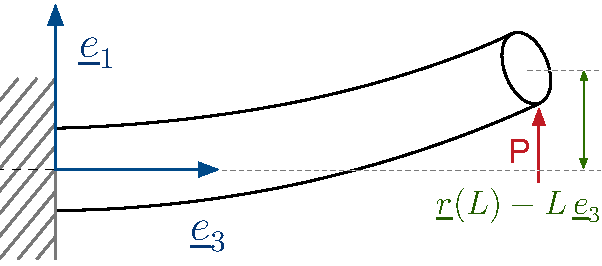
\includegraphics[width=14cm, keepaspectratio=true]{sections/cosserat_rods/images/MinimumPotentialEnergyMethodExample}
  \end{figure}
  
  the \textbf{total energy of the closed system} is given by
  \begin{displaymath}
    \Pi \bigl( \underline{r}, \, \doubleunderline{R} \bigr) =
    \int_0^L \psi \bigl( \underline{v} , \, \underline{k} \bigr) \dif s - P \, \underline{e}_1 \cdot \underline{r}(L)
  \end{displaymath}
  note regarding minus sign: load performs work on the beam, \newline
  thereby lowering the load's potential and also the potential of the closed system
  
  \vspace{0.3em}
  $\rightarrow$ we now want to identify the \textbf{conditions for a minimum of $\Pi$}
\end{frame}


%-------------------------------------------------------------------------------
\begin{frame}
  \frametitle{Minimum potential energy method (part 2)}
  
  \textbf{perturbed versions of $\underline{r}$ and $\doubleunderline{R}$}
  \begin{displaymath}
    \underline{r}_{\epsilon}(s) = \underline{r}(s) + \epsilon \cdot \delta \underline{r}(s)
  \end{displaymath}
  \vspace{-0.5em}
  \begin{displaymath}
    \doubleunderline{R}_{\epsilon}(s) = \underbrace{\xcancel{\doubleunderline{R}(s) + \epsilon \cdot \delta \doubleunderline{R}(s)}}_{\notin SO(3)} = \underbrace{\exp \bigl( \epsilon \cdot \delta \doubleunderline{\Theta}(s) \bigr)}_{\in SO(3)} \, \doubleunderline{R}(s)
    \quad \text{ with } \quad
    \delta \underline{\Theta} := \axial \bigl( \delta \doubleunderline{\Theta} \bigr)
  \end{displaymath}
  
  \vspace{0.6em}
  \textbf{perturbed version of total energy}
  \begin{displaymath}
    \Pi \bigl( \underline{r}_{\epsilon}, \, \doubleunderline{R}_{\epsilon} \bigr) =
    \int_0^L \psi \bigl( \underline{v}_{\epsilon} , \, \underline{k}_{\epsilon} \bigr) \dif s - P \, \underline{e}_1 \cdot \underline{r}_{\epsilon}(L) \overset{!}{=}
    \Pi \bigl( \underline{r}, \, \doubleunderline{R} \bigr) + \epsilon \cdot \delta \Pi \bigl( \underline{r}, \, \doubleunderline{R} \bigr) + \mathcal{o}(\epsilon)
  \end{displaymath}
  
  \vspace{0.6em}
  \textbf{first variation of total energy}
  \begin{displaymath}
    \delta \Pi = \od{\Pi}{\epsilon} \sVert[3]_{\epsilon=0} =
    \int_0^L \biggl(
    \pd{\psi}{\underline{v}}(s) \cdot \underbrace{ \od{\underline{v}_{\epsilon}}{\epsilon}(s) \sVert[2]_{\epsilon=0} }_{\delta \underline{v}(s)} +
    \pd{\psi}{\underline{k}}(s) \cdot \underbrace{ \od{\underline{k}_{\epsilon}}{\epsilon}(s)\sVert[2]_{\epsilon=0} }_{\delta \underline{k}(s)}
    \biggr) \dif s
    - P \, \underline{e}_1 \cdot \od{\underline{r}_{\epsilon}}{\epsilon}(L) \sVert[3]_{\epsilon=0}
  \end{displaymath}
  
  in the sequel we will work on the terms $\delta \underline{v}(s)$ and $\delta \underline{k}(s)$
\end{frame}


%-------------------------------------------------------------------------------
\begin{frame}
  \frametitle{Minimum potential energy method (part 3)}
  \textbf{perturbed version of $\underline{v}$}
  \begin{displaymath}
    \underline{v}_{\epsilon}(s) =
    \doubleunderline{R}_{\epsilon}^{\mathrm{T}}(s) \cdot \underline{r}_{\epsilon}^{\prime}(s) =
    \doubleunderline{R}^{\mathrm{T}}(s) \cdot \biggl( \exp \bigl( \epsilon \cdot \delta \doubleunderline{\Theta}(s) \bigr) \biggr)^{\mathrm{T}} \cdot \bigl( \underline{r}^{\prime}(s) + \epsilon \cdot \delta \underline{r}^{\prime}(s) \bigr)
  \end{displaymath}
  
  \vspace{0.5em}
  \textbf{first variation of $\underline{v}$}
  \begin{displaymath}
    \label{eq:fist_variation_of_v}
    \delta \underline{v}(s) = 
    \od{\underline{v}_{\epsilon}}{\epsilon}(s) \sVert[3]_{\epsilon=0} =
    \doubleunderline{R}^{\mathrm{T}}(s) \cdot
    \od{}{\epsilon} \biggl( \exp \bigl( \epsilon \cdot \delta \doubleunderline{\Theta}(s) \bigr) \biggr)^{\mathrm{T}} \sVert[3]_{\epsilon=0}
     \cdot \underline{r}^{\prime}(s) +
     \doubleunderline{R}^{\mathrm{T}}(s) \cdot \delta \underline{r}^{\prime}(s)
  \end{displaymath}
  
  \vspace{0.5em}
  \begin{displaymath}
    \od{}{\epsilon} \biggl( \exp \bigl( \epsilon \cdot \delta \doubleunderline{\Theta}(s) \bigr) \biggr)^{\mathrm{T}} \sVert[3]_{\epsilon=0} =
    \od{}{\epsilon} \biggl( \doubleunderline{I} + \epsilon \cdot \delta \doubleunderline{\Theta} + \frac{\epsilon^2}{2} \cdot \delta \doubleunderline{\Theta}^2 + \dots \biggr)^{\mathrm{T}} \sVert[3]_{\epsilon=0} =
    \bigl( \delta \doubleunderline{\Theta} \bigr)^{\mathrm{T}} = -\delta \doubleunderline{\Theta} 
  \end{displaymath}
  
  \vspace{0.5em}
  \begin{displaymath}
    \Rightarrow
    \delta \underline{v}(s) =
    \doubleunderline{R}^{\mathrm{T}}(s) \cdot
    \bigl( - \delta \doubleunderline{\Theta}(s) \cdot \underline{r}^{\prime}(s) + \delta \underline{r}^{\prime}(s) \bigr)
  \end{displaymath}
\end{frame}



%-------------------------------------------------------------------------------
\begin{frame}
  \frametitle{Minimum potential energy method (part 4)}
  
  \textbf{perturbed version of $\doubleunderline{K}$, respectively $\underline{k}$}
  \begin{displaymath}
    \doubleunderline{K}_{\epsilon}(s) =
    \doubleunderline{R}_{\epsilon}^{\mathrm{T}}(s) \cdot \doubleunderline{R}_{\epsilon}^{\prime}(s)
    \quad \text{ and } \quad
    \underline{k}_{\epsilon}(s) = \axial \bigl( \doubleunderline{K}_{\epsilon}(s) \bigr)
  \end{displaymath}
  
  \vspace{0.5em}
  \textbf{first variation of $\underline{k}$}
  \begin{displaymath}
    \label{eq:fist_variation_of_k}
    \delta \underline{k}(s) =
    \od{\underline{k}_{\epsilon}}{\epsilon}(s) \sVert[3]_{\epsilon=0} =
    \od{}{\epsilon} \biggl( \axial \bigl( \doubleunderline{R}_{\epsilon}^{\mathrm{T}}(s) \cdot \doubleunderline{R}_{\epsilon}^{\prime}(s) \bigr) \biggr) \sVert[3]_{\epsilon=0} =
  \end{displaymath}
  \begin{displaymath}
    = \axial \biggl( \od{}{\epsilon} \bigl( \doubleunderline{R}_{\epsilon}^{\mathrm{T}}(s) \cdot \doubleunderline{R}_{\epsilon}^{\prime}(s) \bigr) \sVert[2]_{\epsilon=0} \biggr) \overset{(1)}{=}
    \axial \bigl( \doubleunderline{R}^{\mathrm{T}}(s) \cdot \delta \doubleunderline{\Theta}^{\prime}(s) \cdot \doubleunderline{R} \bigr) \overset{(2)}{=}
    \doubleunderline{R}^{\mathrm{T}}(s) \cdot \delta \underline{\Theta}^{\prime}(s)      
  \end{displaymath}
  
  \vspace{0.5em}
  regarding equality $(2)$ we have ...
  \begin{displaymath}
    \bigl( \doubleunderline{R}^{\mathrm{T}} \cdot \delta \doubleunderline{\Theta}^{\prime} \cdot \doubleunderline{R} \bigr) \cdot \underline{a} =
    \doubleunderline{R}^{\mathrm{T}} \cdot \delta \doubleunderline{\Theta}^{\prime} \cdot \bigl( \doubleunderline{R} \cdot \underline{a} \bigr) =
    \doubleunderline{R}^{\mathrm{T}} \cdot \biggl( \delta \underline{\Theta}^{\prime} \times \bigl( \doubleunderline{R} \cdot \underline{a} \bigr) \biggr) =
    \bigl( \doubleunderline{R}^{\mathrm{T}} \cdot \delta \underline{\Theta}^{\prime} \bigr) \times \underline{a}
  \end{displaymath}
\end{frame}


%-------------------------------------------------------------------------------
\begin{frame}
  \frametitle{Minimum potential energy method (part 5)}
  
  and regarding equality $(1)$ we have ...
  \begin{displaymath}
    \od{}{\epsilon} \bigl( \doubleunderline{R}_{\epsilon}^{\mathrm{T}}(s) \cdot \doubleunderline{R}_{\epsilon}^{\prime}(s) \bigr) \sVert[2]_{\epsilon=0} =
  \end{displaymath}
  \begin{displaymath}
    = \od{}{\epsilon} \Biggl[
      \doubleunderline{R}^{\mathrm{T}} \cdot \biggl( \exp \bigl( \epsilon \cdot \delta \doubleunderline{\Theta} \bigr) \biggr)^{\mathrm{T}}
      \cdot \Biggl(
        \biggl( \exp \bigl( \epsilon \cdot \delta \doubleunderline{\Theta} \bigr) \biggr)^{\prime} \cdot \doubleunderline{R}
        + \exp \bigl( \epsilon \cdot \delta \doubleunderline{\Theta} \bigr) \cdot \doubleunderline{R}^{\prime}
      \Biggr)
    \Biggr] \sVert[4]_{\epsilon=0} =
  \end{displaymath}
  \begin{displaymath}
    = \Bigl[
      \cancel{-\doubleunderline{R}^{\mathrm{T}} \cdot \delta \doubleunderline{\Theta} \cdot \doubleunderline{R}^{\prime}} +
        \doubleunderline{R}^{\mathrm{T}} \cdot
        \biggl(
          \delta \doubleunderline{\Theta}^{\prime} \cdot \doubleunderline{R} +
          \cancel{ \delta \doubleunderline{\Theta} \cdot \doubleunderline{R}^{\prime} } 
        \biggr)
      \Bigr] =
      \doubleunderline{R}^{\mathrm{T}} \cdot
      \delta \doubleunderline{\Theta}^{\prime} \cdot \doubleunderline{R}
  \end{displaymath}
  
  \vspace{0.5em}
  ... where we used ...
  \begin{displaymath}
    \od{}{\epsilon} \biggl( \exp \bigl( \epsilon \cdot \delta \doubleunderline{\Theta}(s) \bigr) \biggr)^{\prime} \sVert[3]_{\epsilon=0} =
    \od{}{\epsilon} \biggl( \doubleunderline{I} + \epsilon \cdot \delta \doubleunderline{\Theta} + \frac{\epsilon^2}{2} \cdot \delta \doubleunderline{\Theta}^2 + \dots \biggr)^{\prime} \sVert[3]_{\epsilon=0} =
  \end{displaymath}
  \begin{displaymath}
    = \od{}{\epsilon} \biggl( \epsilon \cdot \delta \doubleunderline{\Theta}^{\prime} + \frac{\epsilon^2}{2} \cdot \delta \doubleunderline{\Theta}^{\prime 2} + \dots \biggr)^{\prime} \sVert[3]_{\epsilon=0} =
    \delta \doubleunderline{\Theta}^{\prime} 
  \end{displaymath}
\end{frame}


%-------------------------------------------------------------------------------
\begin{frame}
  \frametitle{Minimum potential energy method (part 6)}
  
  plugging back into the \textbf{first variation of total energy} we get ...
  \begin{displaymath}
    \delta \Pi =
    \int_0^L \Biggl(
    \pd{\psi}{\underline{v}}(s) \cdot
    \biggl(
    \doubleunderline{R}^{\mathrm{T}}(s) \cdot
    \bigl( - \delta \doubleunderline{\Theta}(s) \cdot \underline{r}^{\prime}(s) + \delta \underline{r}^{\prime}(s) \bigr)
    \biggr) +
  \end{displaymath}
  \begin{displaymath}
    + \pd{\psi}{\underline{k}}(s) \cdot 
    \biggl(
    \doubleunderline{R}^{\mathrm{T}}(s) \cdot \delta \underline{\Theta}^{\prime}(s)
    \biggr)
    \Biggr) \dif s
    - P \, \underline{e}_1 \cdot \delta \underline{r}(L) =
  \end{displaymath}
  \begin{displaymath}
    = \int_0^L \Biggl(
    \biggl( \doubleunderline{R} \cdot \pd{\psi}{\underline{v}}(s) \biggr) \cdot
    \biggl(
      \delta \underline{r}^{\prime}(s) +
      \underline{r}^{\prime}(s) \times \delta \underline{\Theta}(s)
    \biggr) +
  \end{displaymath}
  \begin{displaymath}
    + \biggl( \doubleunderline{R} \cdot \pd{\psi}{\underline{k}}(s) \biggr) \cdot
    \delta \underline{\Theta}^{\prime}(s)
    \Biggr) \dif s
    - P \, \underline{e}_1 \cdot \delta \underline{r}(L) \overset{\text{IBP}}{=}
  \end{displaymath}
  \begin{displaymath}
    = \biggl[ \doubleunderline{R}(s) \cdot \pd{\psi}{\underline{v}}(s) \cdot \delta \underline{r}(s) \biggr]_0^L -
    \int_0^L \Bigl(
      \bigl( \doubleunderline{R}(s) \cdot \pd{\psi}{\underline{v}}(s) \bigr)^{\prime} \cdot \delta \underline{r}(s)
    \Bigr) \dif s -P \, \underline{e}_1 \cdot \delta \underline{r}(L) \, +
  \end{displaymath}
  \begin{displaymath}
    + \biggl[ \doubleunderline{R}(s) \cdot \pd{\psi}{\underline{k}}(s) \cdot \delta \underline{\Theta}(s) \biggr]_0^L -
    \int_0^L \biggl(
      \Bigl(
        \bigl( \doubleunderline{R}(s) \cdot \pd{\psi}{\underline{k}}(s) \bigr)^{\prime} +
        \underline{r}^{\prime}(s) \times \bigl( \doubleunderline{R}(s) \cdot \pd{\psi}{\underline{v}}(s)  \bigr)
      \Bigr) \cdot \delta \underline{\Theta}(s)
    \biggr) \dif s
  \end{displaymath}
  IBP : integration by parts
\end{frame}


%-------------------------------------------------------------------------------
\begin{frame}
  \frametitle{Minimum potential energy method (part 7)}
  
  to finally obtain the conditions for a minimum of the potential energy we set $\delta \Pi = 0$
  
  \vspace{0.5em}
  the integrals must each be $0$ regardless of the variations $\delta \underline{r}$ and $\delta \underline{\Theta}$ \newline
  this gives us the conditions
  \begin{displaymath}
    \bigl( \doubleunderline{R}(s) \cdot \pd{\psi}{\underline{v}}(s) \bigr)^{\prime} = \underline{0}
  \end{displaymath}
  
  \begin{displaymath}
    \bigl( \doubleunderline{R}(s) \cdot \pd{\psi}{\underline{k}}(s) \bigr)^{\prime} +
        \underline{r}^{\prime}(s) \times \bigl( \doubleunderline{R}(s) \cdot \pd{\psi}{\underline{v}}(s)  \bigr) = \underline{0}
  \end{displaymath}
  which must be satisfied for $s \in [0,L]$ in a point-wise manner
  
  \vspace{0.5em}
  at the boundary $s=0$ the cross section is fixed $\Rightarrow$ $\delta \underline{r}(0) \overset{!}{=} \underline{0}$ and $\delta \underline{\Theta}(0) \overset{!}{=} \underline{0}$ \newline
  at the boundary $s=L$ we get the condition
  \begin{displaymath}
    \biggl(
      \doubleunderline{R}(L) \cdot \pd{\psi}{\underline{v}}(L) 
      -P \, \underline{e}_1
    \biggr) \cdot \delta \underline{r}(L) +
    \doubleunderline{R}(L) \cdot \pd{\psi}{\underline{k}}(L) \cdot \delta \underline{\Theta}(L) =
    \underline{0}
  \end{displaymath}
  because $\delta \underline{r}(L)$ and $\delta \underline{\Theta}(L)$ are independent we get
  \begin{displaymath}
    \doubleunderline{R}(L) \cdot \pd{\psi}{\underline{v}}(L) 
      = P \, \underline{e}_1
    \quad \text{ and } \quad
    \doubleunderline{R}(L) \cdot \pd{\psi}{\underline{k}}(L) = \underline{0}
  \end{displaymath}
\end{frame}


%-------------------------------------------------------------------------------
\begin{frame}
  \frametitle{Minimum potential energy method (part 8)}
  
  inside the domain $s \in [0,L]$ we obtained the conditions
  \begin{displaymath}
    \bigl( \doubleunderline{R}(s) \cdot \pd{\psi}{\underline{v}}(s) \bigr)^{\prime} = \underline{0}
  \end{displaymath}
  \begin{displaymath}
    \bigl( \doubleunderline{R}(s) \cdot \pd{\psi}{\underline{k}}(s) \bigr)^{\prime} +
        \underline{r}^{\prime}(s) \times \bigl( \doubleunderline{R}(s) \cdot \pd{\psi}{\underline{v}}(s)  \bigr) = \underline{0}
  \end{displaymath}
  
  \vspace{0.5em}
  balance of linear / angular momentum gives
  \begin{displaymath}
    \underline{n}^{\prime}(s) + \cancel{\underline{\hat{n}}(s)} = \underline{0}
  \end{displaymath}
  \begin{displaymath}
    \underline{m}^{\prime}(s) + \underline{r}^{\prime}(s) \times \underline{n}(s) + \cancel{\underline{\hat{m}}(s)} = \underline{0}
  \end{displaymath}
  note: there are no distributed loads in the example
    
  \vspace{0.5em}
  we identify the relations
  \begin{displaymath}
    \underline{n}(s) = \doubleunderline{R}(s) \cdot \pd{\psi}{\underline{v}}(s)
  \end{displaymath}
  \begin{displaymath}
    \underline{m}(s) = \doubleunderline{R}(s) \cdot \pd{\psi}{\underline{k}}(s)
  \end{displaymath}
\end{frame}

%-------------------------------------------------------------------------------
\begin{frame}
  \frametitle{Relationship between potential energy and kinetic quantities}
 
  \begin{displaymath}
    \underline{n}(s) = \doubleunderline{R}(s) \cdot \pd{\psi}{\underline{v}}(s) =
    n_i \, \underline{e}_i = N_i \, \underline{d}_i
  \end{displaymath}
  \begin{displaymath}
    \underline{m}(s) = \doubleunderline{R}(s) \cdot \pd{\psi}{\underline{k}}(s) =
    m_i \, \underline{e}_i = M_i \, \underline{d}_i
  \end{displaymath}
  
  with $\underline{d}_i(s) = \doubleunderline{R}(s) \cdot \underline{e}_i$ ; it follows that
  \begin{displaymath}
    N_i(s) = \pd{\psi}{v_i}(s)
  \end{displaymath}
  \begin{displaymath}
    M_i(s) = \pd{\psi}{k_i}(s)
  \end{displaymath}
  
  \vspace{0.5em}
  \begin{itemize}
    \item $N_1$, $N_2$ are the shear forces in direction $\underline{d}_1$, $\underline{d}_2$, respectively
    \item $N_3$ is the axial force (in direction $d_3$)
    \item $M_1$, $M_2$ are the bending moments about the $\underline{d}_1$-, $\underline{d}_2$-axis, respectively
    \item $M_3$ is the twisting moment about the $d_3$-axis
  \end{itemize}
\end{frame}

%-------------------------------------------------------------------------------
\begin{frame}
  \frametitle{Energy potential for isotropic circular beams}

  \begin{displaymath}
    \psi \bigl( \underline{v}, \, \underline{k} \bigr) =
    \frac{1}{2} \mathscr{C} \, v_1^2 +
    \frac{1}{2} \mathscr{C} \, v_2^2 +
    \frac{1}{2} \mathscr{D} \, (v_3-1)^2 +
    \frac{1}{2} \mathscr{A} \, k_1^2 +
    \frac{1}{2} \mathscr{A} \, k_2^2 +
    \frac{1}{2} \mathscr{B} \, k_3^2
  \end{displaymath}
  
  \vspace{0.5em}
  \begin{itemize}
    \item shearing stiffness \newline
      $N_1(s) = \pd{\psi}{v_1}(s) = \mathscr{C} \, v_1(s) \overset{!}{=} k \, G \, A \, v_1(s)
      \: \Rightarrow \:
      \mathscr{C} = k \, G \, A$
      
    \item stretching stiffness \newline
      $N_3(s) = \pd{\psi}{v_3}(s) = \mathscr{D} \, (v_3(s) -1) \overset{!}{=} E \, A \, ( v_3(s) -1)
      \: \Rightarrow \:
      \mathscr{D} = E \, A$
      
    \item bending stiffness \newline
      $M_1(s) = \pd{\psi}{k_1}(s) = \mathscr{A} \, k_1(s) \overset{!}{=} E \, I \, k_1(s)
      \: \Rightarrow \:
      \mathscr{A} = E \, I$
      
    \item twisting stiffness \newline
      $M_3(s) = \pd{\psi}{k_3}(s) = \mathscr{B} \, k_3(s) \overset{!}{=} G \, J \, k_3(s)
      \: \Rightarrow \:
      \mathscr{B} = G \, J$
  \end{itemize}
  
  \vspace{1em}
  similarly in 3D-elasticity we have as a constitutive law
  \begin{displaymath}
    \doubleunderline{P} = \pd{W(\doubleunderline{F})}{\doubleunderline{F}}
  \end{displaymath}
\end{frame}


%===============================================================================
\subsection{Combined model}

%-------------------------------------------------------------------------------
\begin{frame}
  \frametitle{Model equations}
  
  \textbf{force balance} with constitutive law
  \begin{displaymath}
    \biggl( \doubleunderline{R}(s) \cdot \pd{\psi}{\underline{v}}(s) \biggr)^{\prime} + \underline{\hat{n}}(s) = 
    \doubleunderline{R}^{\prime}(s) \cdot \pd{\psi}{\underline{v}}(s) +
    \doubleunderline{R}(s) \cdot \biggl( \pd{\psi}{\underline{v}}(s) \biggr)^{\prime} +
    \underline{\hat{n}}(s) =
    \underline{0}
  \end{displaymath}
  
  \vspace{1em}
  \textbf{moment balance} with constitutive law
  \begin{displaymath}
    \biggl( \doubleunderline{R}(s) \cdot \pd{\psi}{\underline{k}}(s) \biggr)^{\prime} +
    \underline{r}^{\prime}(s) \times \biggl( \doubleunderline{R}(s) \cdot \pd{\psi}{\underline{v}}(s) \biggr) +
    \underline{\hat{m}}(s) =
  \end{displaymath}
  \begin{displaymath}
    = 
    \doubleunderline{R}^{\prime}(s) \cdot \pd{\psi}{\underline{k}}(s) +
    \doubleunderline{R}(s) \cdot \biggl( \pd{\psi}{\underline{k}}(s) \biggr)^{\prime} +
    \underline{r}^{\prime}(s) \times \biggl( \doubleunderline{R}(s) \cdot \pd{\psi}{\underline{v}}(s) \biggr) +
    \underline{\hat{m}}(s) =
    \underline{0}
  \end{displaymath}
  
  \vspace{1em}
  we now want to write the equations in terms of $\underline{v}$ and $\underline{k}$ ...
\end{frame}


%-------------------------------------------------------------------------------
\begin{frame}
  \frametitle{Force balance}
  multiplying with $\doubleunderline{R}^{\mathrm{T}}$ on the left we get ...
  \begin{displaymath}
    \doubleunderline{R}^{\mathrm{T}}(s) \cdot
    \doubleunderline{R}^{\prime}(s) \cdot \pd{\psi}{\underline{v}}(s) +
    \biggl( \pd{\psi}{\underline{v}}(s) \biggr)^{\prime} +
    \doubleunderline{R}^{\mathrm{T}}(s) \cdot \underline{\hat{n}}(s) =
  \end{displaymath}
  \begin{displaymath}
    = \underline{k}(s) \times \pd{\psi}{\underline{v}}(s) +
    \pd[2]{\psi}{\underline{v}}(s) \cdot \underline{v}^{\prime}(s) +
    \md{\psi}{2}{\underline{v}}{}{\underline{k}}{}(s) \cdot \underline{k}^{\prime}(s) +
    \underline{\tilde{n}}(s) =
    \underline{0}
  \end{displaymath}
  
  with
  \begin{displaymath}
    \underline{\tilde{n}}(s) :=
    \doubleunderline{R}^{\mathrm{T}}(s) \cdot \underline{\hat{n}}(s)
  \end{displaymath}
\end{frame}


%-------------------------------------------------------------------------------
\begin{frame}
  \frametitle{Moment balance}
  again multiplying with $\doubleunderline{R}^{\mathrm{T}}$ on the left we get ...
  \begin{displaymath}
    \doubleunderline{R}^{\mathrm{T}}(s) \cdot
    \doubleunderline{R}^{\prime}(s) \cdot \pd{\psi}{\underline{k}}(s) +
    \biggl( \pd{\psi}{\underline{k}}(s) \biggr)^{\prime} +
  \end{displaymath}
  \begin{displaymath}
    + \doubleunderline{R}^{\mathrm{T}}(s) \cdot \Biggl(
    \underline{r}^{\prime}(s) \times \biggl( \doubleunderline{R}(s) \cdot \pd{\psi}{\underline{v}}(s) \biggr) \Biggr) +
    \doubleunderline{R}^{\mathrm{T}}(s) \cdot
    \underline{\hat{m}}(s) =
  \end{displaymath}
  \begin{displaymath}
    = \underline{k}(s) \times \pd{\psi}{\underline{k}}(s) +
    \md{\psi}{2}{\underline{v}}{}{\underline{k}}{}(s) \cdot \underline{v}^{\prime}(s) +
    \pd[2]{\psi}{\underline{k}}(s) \cdot \underline{k}^{\prime}(s) +
  \end{displaymath}
  \begin{displaymath}
    + \underline{v}(s) \times \pd{\psi}{\underline{v}}(s) +
    \underline{\tilde{m}}(s) =
    \underline{0}
  \end{displaymath}
  
  with
  \begin{displaymath}
    \underline{\tilde{m}}(s) :=
    \doubleunderline{R}^{\mathrm{T}}(s) \cdot \underline{\hat{m}}(s)
  \end{displaymath}
\end{frame}


%-------------------------------------------------------------------------------
\begin{frame}
  \frametitle{Model equations}
  
  \textbf{force balance}
  \begin{displaymath}
    \underline{k}(s) \times \pd{\psi}{\underline{v}}(s) +
    \pd[2]{\psi}{\underline{v}}(s) \cdot \underline{v}^{\prime}(s) +
    \md{\psi}{2}{\underline{v}}{}{\underline{k}}{}(s) \cdot \underline{k}^{\prime}(s) +
    \underline{\tilde{n}}(s) =
    \underline{0}
  \end{displaymath}
  
  \vspace{0.3em}
  and \textbf{moment balance}
  \begin{displaymath}
    \underline{k}(s) \times \pd{\psi}{\underline{k}}(s) +
    \md{\psi}{2}{\underline{v}}{}{\underline{k}}{}(s) \cdot \underline{v}^{\prime}(s) +
    \pd[2]{\psi}{\underline{k}}(s) \cdot \underline{k}^{\prime}(s) +
  \end{displaymath}
  \begin{displaymath}
    + \underline{v}(s) \times \pd{\psi}{\underline{v}}(s) +
    \underline{\tilde{m}}(s) =
    \underline{0}
  \end{displaymath}
  
  \vspace{0.3em}
  expressed in terms of the \textbf{strains} (in the director basis)
  \begin{displaymath}
    \underline{v}(s) =
    \doubleunderline{R}^{\mathrm{T}}(s) \cdot \underline{r}^{\prime}(s)
    \quad \text{ ; } \quad
    \underline{k}(s) =
    \axial \bigl(
    \doubleunderline{R}^{\mathrm{T}}(s) \cdot \doubleunderline{R}^{\prime}(s)
    \bigr)
  \end{displaymath}
  
  \vspace{0.3em}
  given the \textbf{distributed external loads} (resolved in the director basis)
  \begin{displaymath}
    \underline{\tilde{n}}(s) =
    \doubleunderline{R}^{\mathrm{T}}(s) \cdot \underline{\hat{n}}(s)
    \quad \text{ ; } \quad
    \underline{\tilde{m}}(s) =
    \doubleunderline{R}^{\mathrm{T}}(s) \cdot \underline{\hat{m}}(s)
  \end{displaymath}
  
  \vspace{0.2em}
  $\rightarrow$ system of $6$ equations ;
  $1^{\text{st}}$ order in $\underline{v}$, $\underline{k}$
  but $2^{\text{nd}}$ order in $\underline{r}$, $\doubleunderline{R}$ \newline
  $\: \rightarrow$ $12$ boundary conditions required
\end{frame}

%-------------------------------------------------------------------------------
\begin{frame}
  \frametitle{Example with boundary conditions}

  \begin{figure}
    \centering
    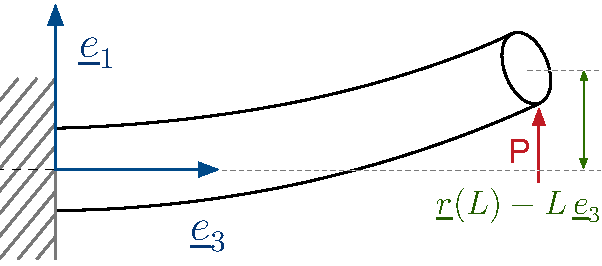
\includegraphics[width=14cm, keepaspectratio=true]{sections/cosserat_rods/images/MinimumPotentialEnergyMethodExample}
  \end{figure}
  
  \vspace{1em}
  we have 12 boundary conditions:
  
  \vspace{0.5em}
  \begin{tabularx}{\linewidth}{XX}
    {
      boundary conditions at $s=0$:
      \begin{itemize}
        \item $\underline{r}(0) = \underline{0}$
        \item $\doubleunderline{R}(0) = \doubleunderline{I} =
          \exp{\doubleunderline{\Theta}} \iff \underline{\Theta}=\underline{0}$
      \end{itemize}
    } & {
      boundary conditions at $s=L$:
      \begin{itemize}
        \item $\doubleunderline{R} \cdot \pd{\psi}{\underline{v}}(L) = P \cdot \underline{e}_1$
        \item $\pd{\psi}{\underline{k}}(L) = \underline{0} \iff M_i = 0 \: (i \in {1,2,3})$
      \end{itemize}
    }
  \end{tabularx}
  
  note that the boundary conditions are not stated in our unknown variables $\underline{v}$, $\underline{k}$
\end{frame}


%-------------------------------------------------------------------------------
\begin{frame}
  \frametitle{Model as a system of first order equations (part 1)}
  
  boundary conditions for forces and moments can be written in terms of strains ; this is not possible with the boundary conditions for displacements and rotations ; therefore the system is not closed
  
  \vspace{0.7em}
  to \textit{close the system}, we will rewrite the model as 12 first order equations, \newline
  by including 6 extra equations relating strain quantities to displacement quantities:
  \begin{displaymath}
    \underline{v} = \doubleunderline{R}^{\mathrm{T}} \cdot \underline{r}^{\prime}
    \Rightarrow
    \underline{r}^{\prime} = \doubleunderline{R} \cdot \underline{v}
  \end{displaymath}
  \begin{displaymath}
    \doubleunderline{K} = \doubleunderline{R}^{\mathrm{T}} \cdot \doubleunderline{R}^{\prime}
    \Rightarrow
    \doubleunderline{R}^{\prime} = \doubleunderline{R} \cdot \doubleunderline{K}
  \end{displaymath}
  
  \vspace{0.7em}
  we already noticed, that using unit quaternions to encode $SO(3)$ matrices has some great advantages for computation. therefore we chose to replace the matrix differential equation in $\doubleunderline{R}$ by a matrix differential equation in terms of unit quaternions $\underline{q} \in \mathbb{R}^4$
  \begin{displaymath}
    \underline{q}^{\prime} = \doubleunderline{E}(\underline{q}) \cdot \underline{k} =
    \frac{1}{2} \cdot \begin{bmatrix}
      -q_1 & -q_2 & -q_3 \\
      +q_0 & -q_3 & +q_2 \\
      +q_3 & +q_0 & -q_1 \\
      -q_2 & +q_1 & +q_0
    \end{bmatrix} \cdot \underline{k}
  \end{displaymath}
\end{frame}

%-------------------------------------------------------------------------------
\begin{frame}
  \frametitle{Model as a system of first order equations (part 2)}

  we have the same 6 equations as before here expressed in matrix form
  
  \begin{displaymath}
    \underbrace{
    \begin{bmatrix}
      \pd[2]{\psi}{\underline{v}} &
      \md{\psi}{2}{\underline{v}}{}{\underline{k}}{} \\
      \md{\psi}{2}{\underline{k}}{}{\underline{v}}{} &
      \pd[2]{\psi}{\underline{k}}
    \end{bmatrix}
    }_{=: \doubleunderline{C}}
    \cdot
    \begin{bmatrix}
      \underline{v}^{\prime} \\
      \underline{k}^{\prime}
    \end{bmatrix} =
    \begin{bmatrix}
      -\underline{k} \times \pd{\psi}{\underline{v}} \\
      -\underline{k} \times \pd{\psi}{\underline{k}}
      -\underline{v} \times \pd{\psi}{\underline{v}}
    \end{bmatrix} -
    \begin{bmatrix}
      \doubleunderline{R}^{\mathrm{T}} \, \underline{\hat{n}} \\
      \doubleunderline{R}^{\mathrm{T}} \, \underline{\hat{m}}
    \end{bmatrix}
  \end{displaymath}
  
  $\doubleunderline{C}$ is the (positive definite) elasticity tensor matrix
  
  \vspace{1em}
  we close the system by adding the seven extra first order equations \newline
  (relating derivatives of displacements to strains)
  \begin{displaymath}
    \underline{r}^{\prime} = \doubleunderline{R} \cdot \underline{v}
  \end{displaymath}
  \begin{displaymath}
    \underline{q}^{\prime} = \doubleunderline{E}(\underline{q}) \cdot \underline{k}
  \end{displaymath}
  
  \vspace{1em}
  $\rightarrow$ this gives us a system of 13 coupled nonlinear ODEs
\end{frame}


%-------------------------------------------------------------------------------
\begin{frame}
  \frametitle{Extra constraint for unit quaternions}
  
  using unit quaternions to encode rotations leads to a system of 13 equations \newline
  instead of just 12 ; this extra equation is contained within
  \begin{displaymath}
    \underline{q}^{\prime} = \doubleunderline{E}(\underline{q}) \cdot \underline{k} \quad (\star)
  \end{displaymath}
  
  since rotations are encoded by \textit{unit} quaternions the constraint $\norm[1]{\underline{q}}_{2} \overset{!}{=} 1$ must be satisfied
  
  from the constraint we obtain a necessary condition: $\underline{q} \cdot \underline{q} \overset{!}{=} 1 \: \Rightarrow \: \underline{q} \cdot \underline{q}^{\prime} \overset{!}{=} 0$, which is automatically satisfied by $(\star)$: \quad dotting $(\star)$ with $\underline{q}$ gives ...
  \begin{displaymath}
    \underline{q}^{\prime} \cdot \underline{q} =
    \bigl( \doubleunderline{E}(\underline{q}) \cdot \underline{k} \bigr) \cdot \underline{q} =
    \underline{k} \cdot \bigl( \doubleunderline{E}^{\mathrm{T}} \cdot \underline{q} \bigr) =
    \underline{k} \cdot \Biggl(
    \begin{bmatrix}
      -q_1 & +q_0 & +q_3 & -q_2\\
      -q_2 & -q_3 & +q_0 & +q_1\\
      -q_3 & +q_2 & -q_1 & +q_0
    \end{bmatrix} \cdot
    \begin{bmatrix}
      q_0 \\ q_1 \\ q_2 \\ q_3
    \end{bmatrix}
    \Biggr) =
    \underline{k} \cdot
    \begin{bmatrix}
      0 \\ 0 \\ 0
    \end{bmatrix} = 0
  \end{displaymath}
  adding one ($13^{\text{th}}$) boundary condition for $\underline{q}$ (either $\norm[1]{\underline{q}}_{2} \sVert[2]_{s=0} = 1$ or $\: \norm[1]{\underline{q}}_{2} \sVert[2]_{s=L} = 1$) is (in combination with the automatically satisfied necessary condition) sufficient to satisfy the constraint for all $s$
\end{frame}


%-------------------------------------------------------------------------------
\begin{frame}
  \frametitle{Example with boundary conditions (revisited)}

  \begin{figure}
    \centering
    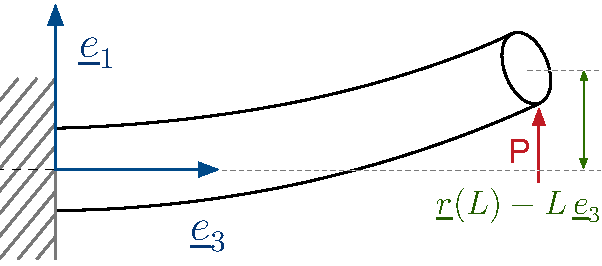
\includegraphics[width=11cm, keepaspectratio=true]{sections/cosserat_rods/images/MinimumPotentialEnergyMethodExample}
  \end{figure}
  
  \vspace{0.7em}
  we have 13 boundary conditions:
  
  \vspace{0.5em}
  \begin{tabularx}{\linewidth}{XX}
    {
      boundary conditions at $s=0$:
      \begin{itemize}
        \item $\underline{r}(0) = \underline{0}$
        \item $\underline{q}(0) =
          \begin{bmatrix}
            1 & 0 & 0 & 0
          \end{bmatrix}^{\mathrm{T}}$ because
          \begin{itemize}
            \item $\: \: \, q_0 = \cos\bigl( \frac{\Theta}{2} \bigr) = 1$ and
            \item $\begin{bmatrix}
            q_1 \\ q_2 \\ q_3
          \end{bmatrix} = \sin \bigl( \frac{\Theta}{2} \bigr) \cdot \underline{a} =
          \begin{bmatrix}
            0 \\ 0 \\ 0
          \end{bmatrix}$
        \end{itemize}
      \end{itemize}
    } & {
      boundary conditions at $s=L$:
      \begin{itemize}
        \item $\doubleunderline{R} \cdot \pd{\psi}{\underline{v}}(L) = P \cdot \underline{e}_1$
        \item $\pd{\psi}{\underline{k}}(L) = \underline{0} \iff$
          \begin{itemize}
            \item $M_i(L) = 0 \: (i \in {1,2,3})$
          \end{itemize}
      \end{itemize}
    }
  \end{tabularx}
\end{frame}


%-------------------------------------------------------------------------------
\begin{frame}
  \frametitle{Another example with boundary conditions: follower load problem}
  \vspace{-1em}
  \begin{multicols}{2}
    \noindent  
    \begin{figure}
      \centering
      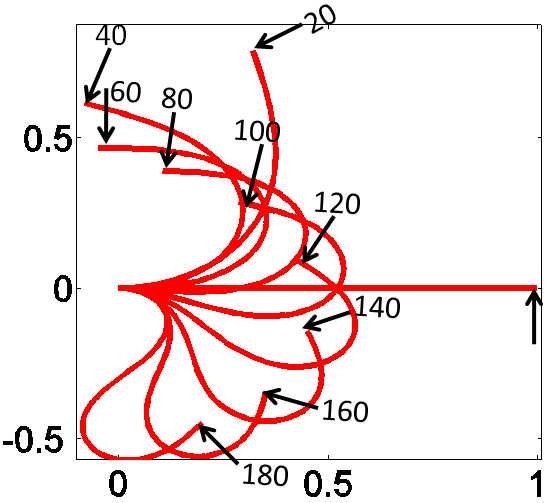
\includegraphics[width=11cm, keepaspectratio=true]{sections/cosserat_rods/images/FollowerLoadExample}
    \end{figure}
    
    boundary conditions at $s=0$:
    \begin{itemize}
      \item $\underline{r}(0) = \underline{0}$
      \item $\underline{q}(0) =
        \begin{bmatrix}
          1 & 0 & 0 & 0
        \end{bmatrix}^{\mathrm{T}}$ because
        \begin{itemize}
          \item $\: \: \, q_0 = \cos\bigl( \frac{\Theta}{2} \bigr) = 1$ and
          \item $\begin{bmatrix}
          q_1 \\ q_2 \\ q_3
        \end{bmatrix} = \sin \bigl( \frac{\Theta}{2} \bigr) \cdot \underline{a} =
        \begin{bmatrix}
          0 \\ 0 \\ 0
        \end{bmatrix}$
      \end{itemize}
    \end{itemize}
    
    \vspace{1em}
    boundary conditions at $s=L$:
      \begin{itemize}
        \item $\doubleunderline{R} \cdot \pd{\psi}{\underline{v}}(L) = P \cdot \underline{d}_1 = \doubleunderline{R} \cdot P \cdot \underline{e}_1 \: \Rightarrow$
          \begin{itemize}
            \item $\pd{\psi}{v_1}(L) = P$
            \item $\pd{\psi}{v_2}(L) = 0$
            \item $\pd{\psi}{v_3}(L) = 0$
          \end{itemize}
        \item $\pd{\psi}{\underline{k}}(L) = \underline{0} \iff$
          \begin{itemize}
            \item $M_i(L) = 0 \: (i \in {1,2,3})$
          \end{itemize}
      \end{itemize}
  \end{multicols}
\end{frame}


%-------------------------------------------------------------------------------
\begin{frame}
  \frametitle{Yet another example with boundary conditions}
  \vspace{-0.5em}
  \begin{multicols}{2}
    \noindent
    \begin{figure}
      \centering
      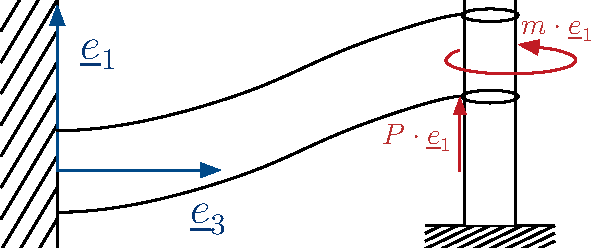
\includegraphics[width=11cm, keepaspectratio=true]{sections/cosserat_rods/images/YetAnotherExampleWithBC}
    \end{figure}
  
    boundary conditions at $s=0$:
    \begin{itemize}
      \item $\underline{r}(0) = \underline{0}$
      \item $\underline{q}(0) =
        \begin{bmatrix}
          1 & 0 & 0 & 0
        \end{bmatrix}^{\mathrm{T}}$ because
        \begin{itemize}
          \item $\: \: \, q_0 = \cos\bigl( \frac{\Theta}{2} \bigr) = 1$ and
          \item $\begin{bmatrix}
          q_1 \\ q_2 \\ q_3
        \end{bmatrix} = \sin \bigl( \frac{\Theta}{2} \bigr) \cdot \underline{a} =
        \begin{bmatrix}
          0 \\ 0 \\ 0
        \end{bmatrix}$
      \end{itemize}
    \end{itemize}
    \vspace{2em}

    boundary conditions at $s=L$:
    \begin{itemize}
      \item $n_1(L) = P$
        \begin{itemize}
          \item $\doubleunderline{R} \cdot \pd{\psi}{\underline{v}}(L) = P \cdot \underline{e}_1 \: \Rightarrow$
          \item $\bigl( \doubleunderline{R} \cdot \pd{\psi}{\underline{v}}(L) \bigr) \cdot \underline{e}_1 = P \: \wedge \: \underline{e}_1 = \underline{d}_1(L) \Rightarrow$
          \item $\pd{\psi}{v_1}(L) = P$
        \end{itemize}
      \item $r_2(L) = 0$
      \item $r_3(L) = L$
      \item $\pd{\psi}{k_1}(L) = m$
      \item $\begin{bmatrix}
              q_1 \\ q_2 \\ q_3
            \end{bmatrix} =
            \sin \bigl( \frac{\Theta}{2} \bigr) \cdot
            \begin{bmatrix}
              1 \\ 0 \\ 0
            \end{bmatrix}
            \: \Rightarrow \: q_2 =0 , \, q_3 = 0$
    \end{itemize}
  \end{multicols}
\end{frame}


%===============================================================================
\subsection{Constitutive laws (part 2)}

%-------------------------------------------------------------------------------
\begin{frame}
  \frametitle{Material symmetry in 3D elasticity}

  \begin{displaymath}
    W \bigl( \doubleunderline{F} \bigr) \overset{\star}{=}
    W \bigl( \doubleunderline{U} \bigr) \overset{\diamond}{=}
    W \bigl( I_1, \, I_2, \, I_3 \bigr)
  \end{displaymath}
  
  \vspace{0.5em}
  \begin{itemize}
    \item $\star$ : principle of frame-indifference
    \item $\doubleunderline{U}$ : from polar decomposition $\doubleunderline{F} = \doubleunderline{\tilde{R}} \cdot \doubleunderline{U}$
    \item $\diamond$ : isotropy: material law is the same for all directions in the material
    \item $I_1$, $I_2$, $I_3$ : strain-invariants
    \item in case of an orthotropic material law, there would simply result a few more invariants ; \newline
      othotropy here means that the material behavior in $s$ direction differs from the behavior in $X_1$, $X_2$ directions
  \end{itemize}
  
  \vspace{1em}
  \textbf{how to obtain the specific form of the energy potential function}? \newline
  remember for example the already postulated function
  \vspace{0.53em}
  \begin{displaymath}
    \psi \bigl( \underline{v}, \, \underline{k} \bigr) =
    \frac{1}{2} \mathscr{C} \, v_1^2 +
    \frac{1}{2} \mathscr{C} \, v_2^2 +
    \frac{1}{2} \mathscr{D} \, (v_3-1)^2 +
    \frac{1}{2} \mathscr{A} \, k_1^2 +
    \frac{1}{2} \mathscr{A} \, k_2^2 +
    \frac{1}{2} \mathscr{B} \, k_3^2
  \end{displaymath}
  
  \vspace{0.3em}
  $\rightarrow$ how to identify the strain invariants? \newline
\end{frame}


%-------------------------------------------------------------------------------
\begin{frame}
  \frametitle{Material symmetry in elastic rods (part 1)}
  
  to get a better understanding of the concept of material symmetry, \newline
  we set up \textbf{another thought experiment}
  \vspace{0.5em}
  \begin{figure}
    \centering
    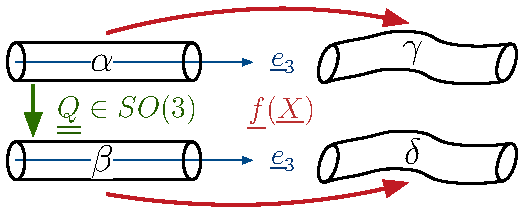
\includegraphics[width=18cm, keepaspectratio=true]{sections/cosserat_rods/images/MaterialSymmetryExperiment}
  \end{figure}
  \begin{itemize}
    \item we start with the reference configuration $\alpha$
    \item we rotate $\alpha$ by $\doubleunderline{Q}$ to get $\beta$ (a rotated reference configuration)
    \item $\underline{f}(.)$ maps $\alpha \mapsto \gamma$ and $\beta \mapsto \delta$
  \end{itemize}
  
  if $\doubleunderline{Q}$ is in the symmetry group $\mathscr{G}$ then then we have $\eval[1]{\psi}_{\gamma} = \eval[1]{\psi}_{\delta}$
\end{frame}


%-------------------------------------------------------------------------------
\begin{frame}
  \frametitle{Material symmetry in elastic rods (part 2)}

  \begin{enumerate}
    \item configuration $\gamma$ (image of reference configuration $\alpha$)
      \begin{itemize}
        \item $\underline{r}^{\gamma}(s)$
        \item $\doubleunderline{R}^{\gamma}(s)$
      \end{itemize}
    \item configuration $\delta$ (image of rotated reference configuration $\beta$)
      \begin{itemize}
        \item $\underline{r}^{\delta}(s) =
                \underline{r}^{\gamma}(s)$
        \item $\doubleunderline{R}^{\delta}(s) =
                \doubleunderline{R}^{\gamma}(s) \cdot \doubleunderline{Q}$
        \item $\underline{v}^{\delta}(s) =
                \doubleunderline{R}^{\gamma \mathrm{T}}(s) \cdot \underline{r}^{\gamma \prime}(s) =
                \doubleunderline{Q}^{\mathrm{T}} \cdot \doubleunderline{R}^{\gamma \mathrm{T}}(s) \cdot \underline{r}^{\gamma \prime}(s) =
                \doubleunderline{Q}^{\mathrm{T}} \cdot \underline{v}^{\gamma}(s)$
        \item $\underline{k}^{\delta} =
                \axial \bigl( \doubleunderline{R}^{\delta \mathrm{T}} \cdot \doubleunderline{R}^{\delta \prime} \bigr) =
                \axial \bigl( \doubleunderline{Q}^{\mathrm{T}} \cdot \doubleunderline{R}^{\gamma \mathrm{T}} \cdot \doubleunderline{R}^{\gamma \prime} \cdot \doubleunderline{Q} \bigr) =
                \doubleunderline{Q}^{\mathrm{T}} \cdot \axial \bigl( \doubleunderline{R}^{\gamma \mathrm{T}} \cdot \doubleunderline{R}^{\gamma \prime} \bigr) =
                \doubleunderline{Q}^{\mathrm{T}} \cdot \underline{k}^{\gamma}$
      \end{itemize}
  \end{enumerate}
  
  \begin{displaymath}
    \Rightarrow
    \psi \bigl( \doubleunderline{Q}^{\mathrm{T}} \cdot \underline{v}^{\gamma}, \, \doubleunderline{Q}^{\mathrm{T}} \cdot \underline{k}^{\gamma} \bigr) \overset{!}{=}
    \psi \bigl( \underline{v}^{\gamma}, \, \underline{k}^{\gamma} \bigr)
    \: \forall \doubleunderline{Q} \in \mathscr{G}
  \end{displaymath}
  
  \vspace{0.5em}
  \begin{itemize}
    \item the symmetry group $\mathscr{G}$ depends on geometry and on the material of the beam
    \item $\mathscr{G} \equiv SO(2)$ (all rotations about $\underline{e}_3$-axis), if beam has circular cross section and isotropic material ; also the case for circular ropes with continuous helicity
  \end{itemize}
  
\end{frame}


%-------------------------------------------------------------------------------
\begin{frame}
  \frametitle{Material symmetry in elastic rods (part 3)}
  \vspace{-0.4em}
  with $\mathscr{G} \equiv SO(2)$ we had ...
  \begin{displaymath}
    \doubleunderline{Q} =
    \begin{bmatrix}
      +\cos(\Theta) & -\sin(\Theta) & 0 \\
      +\sin(\Theta) & +\cos(\Theta) & 0 \\
      0 & 0 & 1
    \end{bmatrix}
    \quad \forall \: \Theta \in [0,2\,\pi]
  \end{displaymath}
  \begin{displaymath}
    \underline{v}^{\delta} =
    \doubleunderline{Q}^{\mathrm{T}} \cdot \underline{v}^{\gamma} =
    \begin{bmatrix}
      \begin{bmatrix}
        +\cos(\Theta) & +\sin(\Theta) \\
        -\sin(\Theta) & +\cos(\Theta)
      \end{bmatrix} \cdot
      \begin{bmatrix}
        v_1^{\gamma} \\ v_2^{\gamma}
      \end{bmatrix} \\
      v_3^{\gamma}
    \end{bmatrix}
    \: ; \quad
    \underline{v}^{\delta} = \dots \text{(replace }v\text{ by }k\text{)}
  \end{displaymath}
  we introduce some abbreviations ...
  \begin{displaymath}
    \underline{v}^{\delta} =
    \begin{bmatrix}
      \doubleunderline{\hat{Q}}^{\mathrm{T}} \cdot \underline{\hat{v}}^{\gamma} \\
      v_3^{\gamma}
    \end{bmatrix}   
    \text{ with }
    \underline{\hat{v}}^{\gamma} =
    \begin{bmatrix}
      v_1^{\gamma} \\ v_2^{\gamma}
    \end{bmatrix}
    \text{ and }
    \doubleunderline{\hat{Q}} =
    \begin{bmatrix}
      +\cos(\Theta) & -\sin(\Theta) \\
      +\sin(\Theta) & +\cos(\Theta)
    \end{bmatrix}
  \end{displaymath}
  
  \vspace{0.4em}
  we observe the following \textbf{invariants} under all such transformations $\doubleunderline{Q} \in \mathscr{G}$
  \begin{itemize}
    \item angle between and magnitude of $\underline{\hat{v}}$, $\underline{\hat{k}}$
      $\quad \rightarrow \quad$
      $\enVert[1]{\underline{\hat{v}}}$ , $\enVert[1]{\underline{\hat{k}}}$ , $\underline{\hat{v}} \cdot \underline{\hat{k}}$ , $\left( \underline{\hat{v}} \times \underline{\hat{k}} \right) \cdot \underline{e}_3$
    \item $v_3$, $k_3$
  \end{itemize}
  
  \vspace{-1em}
  \begin{displaymath}
    \Rightarrow
    \psi = \psi \bigl(
      \underbrace{v_1^2 + v_2^2}_{I_1} , \, \underbrace{k_1^2 + k_2^2}_{I_2} , \, \underbrace{v_1 \cdot k_1 + v_2 \cdot k_2}_{I_3} , \, \underbrace{v_1 \cdot k_2 - v_2 \cdot k_1}_{I_4} , \, \underbrace{v_3}_{I_5} , \, \underbrace{k_3}_{I_6}
    \bigr)
  \end{displaymath}
\end{frame}

%-------------------------------------------------------------------------------
\begin{frame}
  \frametitle{Material symmetry in elastic rods (part 4)}

  to derive the concrete form of the energy potential function, \newline
  we do a Taylor-expansion of $\psi$ about $\bigl( \underline{v}_0 , \, \underline{k}_0 \bigr) = \bigl( \begin{bmatrix}
    0 & 0 & 1
  \end{bmatrix}^{\mathrm{T}} , \, \begin{bmatrix}
    0 & 0 & 0
  \end{bmatrix}^{\mathrm{T}} \bigr)$
  \begin{displaymath}
    \psi \bigl( \underline{v}, \, \underline{k} \bigr) =
    \cancelto{0}{ \psi \bigl( \underline{v}_0, \, \underline{k}_0 \bigr) } +
    \cancelto{0}{ \pd{\psi}{\underline{v}} \bigl( \underline{v}_0, \, \underline{k}_0 \bigr) } \cdot \bigl( \underline{v} - \underline{v}_0 \bigr)  +
    \cancelto{0}{ \pd{\psi}{\underline{k}} \bigl( \underline{v}_0, \, \underline{k}_0 \bigr) } \cdot \bigl( \underline{k} - \underline{k}_0 \bigr) +
  \end{displaymath}
  \begin{displaymath}
    + \frac{1}{2} \Biggl(
      \Bigl( \pd[2]{\psi}{\underline{v}} \cdot \bigl( \underline{v} - \underline{v}_0 \bigr) \Bigr) \cdot \bigl( \underline{v} - \underline{v}_0 \bigr) + 
      \Bigl( \pd[2]{\psi}{\underline{k}} \cdot \bigl( \underline{k} - \underline{k}_0 \bigr) \Bigr) \cdot \bigl( \underline{k} - \underline{k}_0 \bigr) +
  \end{displaymath}
  \begin{displaymath}
      + 2 \cdot \Bigl( \md{\psi}{2}{\underline{v}}{}{\underline{k}}{} \cdot \bigl( \underline{k} - \underline{k}_0 \bigr) \Bigr) \cdot \bigl( \underline{v} - \underline{v}_0 \bigr)
    \Biggr) + \text{HOT}
  \end{displaymath}
  
  \vspace{0.5em}
  from the Taylor expansion consider for example the term
  \begin{displaymath}
    \pd[2]{\psi}{\underline{v}} =
    \pd{}{\underline{v}} \biggl( \pd{\psi}{\underline{v}} \biggr) =
    \pd{}{\underline{v}} \biggl( \pd{\psi}{I_1} \cdot \pd{I_1}{\underline{v}} + \dots + \pd{\psi}{I_6} \cdot \pd{I_6}{\underline{v}} \biggr) = \dots
  \end{displaymath}
  
  $\pd{\psi}{I_j}$ are unknowns that must be obtained from experiments / 3D elasticity,
  whereas $\pd{I_j}{\underline{v}}$ can easily be computed from kinematics ($j = 1,\dots,6$)

\end{frame}


%-------------------------------------------------------------------------------
\begin{frame}
  \frametitle{Material symmetry in elastic rods (part 5)}

  doing the computations and grouping terms in a way to get a polynomial in the strains we obtain
  \begin{displaymath}
    \psi =
    \frac{1}{2} \Bigl(
      \mathscr{A} \cdot \bigl( k_1^2 + k_2^2 \bigr) +
      \mathscr{B} \cdot k_3^2 +
      \mathscr{C} \cdot \bigl( v_1^2 + v_2^2 \bigr) +
      \mathscr{D} \cdot \bigl( k_3 - 1 \bigr)^2 \Bigr) +
  \end{displaymath}
  \begin{displaymath}
    + \cdot \mathscr{E} \cdot \bigl( v_3 - 1 \bigr) \cdot k_3 +
      \cdot \mathscr{F} \cdot \bigl( v_1 \cdot k_1 + v_2 \cdot k_2 \bigr)
    + \text{HOT}
  \end{displaymath}
  
  \vspace{1em}
  as \textbf{another experiment} consider now a reflection of the beam about the $\underline{e}_1$-$\underline{e}_2$-plane
  
  \vspace{0.3em}
  \begin{itemize}
    \item reflections are in the group $O(2)$
    \item reflections are not in the symmetry group $\mathscr{G} \equiv SO(2)$ of a pre-twisted rod
    %\item $I_4 = v_1 \cdot k_2 - v_2 \cdot k_1$, $I_5 = v_3$, $I_6 = k_3$ will change their sign \newline $\rightarrow$ not invariant under transformation by $\doubleunderline{Q} \in O(2)$ (not perfectly correct!) refer to paper:
    % Material symmetry and chirality in nonlinear elastic rods BY Healey 2002 , MMS
   \item $O(2)$ is the symmetry group for rods without helicity of fibers in the undeformed configuration ; for such rods $\mathscr{E} = \mathscr{F} = 0$ 
  \end{itemize}
 
\end{frame}

% TODO without HOT > linear constitutive law > Hessian does not depend on v,k > information obtained from relaxation of CS is useless


%===============================================================================
\subsection{Relaxation of cross section}

%-------------------------------------------------------------------------------
\begin{frame}
  \frametitle{Recap: kinematics}

  \begin{itemize}
    \item $s$ identifies a certain cross section of the rod
    \item $\underline{r}(s)$ describes the position of the cross section centroid for the cross section at $s$
      \begin{itemize}
        \item $\rightarrow$ describes the centerline of the rod
      \end{itemize}
    \item $\doubleunderline{R}(s)$ describes the (average) orientation of the cross section at $s$
      \begin{itemize}
        \item $\rightarrow$ $\underline{d}_i(s) = \doubleunderline{R}(s) \cdot \underline{e}_i$ is the local director basis
      \end{itemize}
  \end{itemize}
  
  \vspace{0.6em}
  \textbf{deformation map} with warping of the cross section
  \begin{displaymath}
    \underline{f}(\underline{X}) = \underline{f}(X_1,X_2,X_3=s) = \underline{r}(s) + \doubleunderline{R}(s) \cdot (X_{\alpha} \, \underline{e}_{\alpha} + \underline{u}) \quad \text{with } \alpha \in \{1,2\}
  \end{displaymath}
  note that so far we did not use any deformation map in the derivations!
  
  \vspace{0.6em}
  local \textbf{strain measures}
  \vspace{-1em}
  \begin{multicols}{2}
    \noindent  
    \begin{itemize}
      \item $\underline{v} = \doubleunderline{R}^{\mathrm{T}} \cdot \underline{r}^{\prime} =
            \begin{bmatrix}
              v_1 & v_2 & v_3
            \end{bmatrix}^{\mathrm{T}}$
          \begin{itemize}
            \item $v_1$ : shear along $\underline{d}_1$
            \item $v_2$ : shear along $\underline{d}_2$
            \item $v_3$ : axial stretch (along $\underline{d}_3$)
          \end{itemize}
      \item $\underline{k} = \axial \bigl( \doubleunderline{R}^{\mathrm{T}} \cdot \doubleunderline{R}^{\prime} \bigr) =
            \begin{bmatrix}
              k_1 & k_2 & k_3
            \end{bmatrix}^{\mathrm{T}}$
          \begin{itemize}
            \item $k_1$ : curvature about $\underline{d}_1$-axis
            \item $k_2$ : curvature about $\underline{d}_2$-axis
            \item $k_3$ : twist about $\underline{d}_3$-axis
          \end{itemize}
    \end{itemize}
  \end{multicols}
\end{frame}


%-------------------------------------------------------------------------------
\begin{frame}
  \frametitle{Recap: balance laws}

  \textbf{balance of linear momentum}
  \begin{displaymath}
    \underline{n}^{\prime}(s) + \underline{\hat{n}}(s) =
    \rho_0 \cdot A \cdot \underline{\ddot{r}}(s)
  \end{displaymath}
  
  \vspace{0.5em}
  \textbf{balance of angular momentum}
  \begin{displaymath}
    \underline{m}^{\prime}(s) + \underline{r}^{\prime}(s) \times \underline{n}(s) + \underline{\hat{m}}(s) =
    \rho_0 \cdot
    \od{}{t} \bigl( \doubleunderline{I}_0 \cdot \underline{\omega} \bigr)
  \end{displaymath}
  
  \vspace{0.5em}
  equations are in terms of the \textbf{internal contact force} and \textbf{internal moment}
  \begin{displaymath}
    \begin{alignedat}{1}
      \underline{n}(s) &= \iint_{\Omega_0(s)} \doubleunderline{P}(X_1, X_2, s) \cdot \underline{e}_3 \dif X_1 \dif X_2 \\
       %\null &= \doubleunderline{R}(s) \cdot \pd{\psi}{\underline{v}}(s) \\
      \underline{m}(s) &= \iint_{\Omega_0(s)} \bigl( \underline{x}(X_1,X_2,s) - \underline{r}(s) \bigr) \times \bigl( \doubleunderline{P}(X_1,X_2,s) \cdot \underline{e}_3 \bigr) \dif X_1 \dif X_2 %\\
      %\null &= \doubleunderline{R}(s) \cdot \pd{\psi}{\underline{k}}(s)
    \end{alignedat}
  \end{displaymath}
  
  \vspace{0.5em}
  with \textbf{external loads}
  \begin{displaymath}
    \begin{alignedat}{1}
      \underline{\hat{n}}(s) &= \iint_{\Omega_{0}(s)} \underline{B}(X_1,X_2,s) \dif A + \oint_{\partial \Omega_{0}(s)} \underline{t}^{ext}(l,s) \dif l \\
      \underline{\hat{m}}(s) &= \iint_{\Omega_{0}(s)} \bigl( \underline{x}(.,.,s) - \underline{r}(s) \bigr) \times \underline{B}(s) \dif A + \oint_{\partial \Omega_0} \bigl( \underline{x}(.,.,s) - \underline{r}(s) \bigr) \times \underline{t}^{ext}(s) \dif l \biggr)
    \end{alignedat}
  \end{displaymath}
  
\end{frame}

%-------------------------------------------------------------------------------
\begin{frame}
  \frametitle{Recap: constitutive laws}
  
  \textbf{strain energy per unit of undeformed length}
  \begin{displaymath}
    \phi \bigl( \underline{r}(s),\doubleunderline{R}(s),\underline{r}^{\prime}(s),\doubleunderline{R}^{\prime}(s) \bigr) \overset{\star}{=}
    \psi \bigl(
      \doubleunderline{R}^{\mathrm{T}}(s) \, \underline{r}^{\prime}(s) , \,
      \doubleunderline{R}^{\mathrm{T}}(s) \, \doubleunderline{R}^{\prime}(s)
    \bigr) =
    \psi \bigl(
      \underline{v}(s) , \underline{k}(s)
    \bigr)
  \end{displaymath}
  $\star$ : principle of frame-indifference
  
  \vspace{0.8em}
  \textbf{relationship between potential energy and kinetic quantities}
  \begin{displaymath}
    \underline{n}(s) = \doubleunderline{R}(s) \cdot \pd{\psi}{\underline{v}}(s) %=
    %n_i \, \underline{e}_i = N_i \, \underline{d}_i
  %\end{displaymath}
  \quad ; \quad
  %\begin{displaymath}
    \underline{m}(s) = \doubleunderline{R}(s) \cdot \pd{\psi}{\underline{k}}(s) %=
    %m_i \, \underline{e}_i = M_i \, \underline{d}_i
  \end{displaymath}
  
  \vspace{0.8em}
  \textbf{material symmetry in elastic rods}
  \begin{displaymath}
    \psi \bigl(
      \underline{v}(s) , \underline{k}(s)
    \bigr) \overset{\mathscr{G} \equiv SO(2)}{=}
    \psi \bigl(
      v_1^2 + v_2^2 , \, k_1^2 + k_2^2 , \, v_1 \cdot k_1 + v_2 \cdot k_2 , \, v_1 \cdot k_2 - v_2 \cdot k_1 , \, v_3 , k_3
    \bigr)
  \end{displaymath}
  \begin{displaymath}
    \approx \frac{1}{2} \Bigl(
      \mathscr{A} \bigl( k_1^2 + k_2^2 \bigr) +
      \mathscr{B} \cdot k_3^2 +
      \mathscr{C} \cdot \bigl( v_1^2 + v_2^2 \bigr) +
      \mathscr{D} \cdot \bigl( k_3 - 1 \bigr)^2 \Bigr) +
  \end{displaymath}
  \begin{displaymath}
    + \cdot \mathscr{E} \cdot \bigl( v_3 - 1 \bigr) \cdot k_3 +
      \cdot \mathscr{F} \cdot \bigl( v_1 \cdot k_1 + v_2 \cdot k_2 \bigr)
  \end{displaymath}
  
  if fibers of the rod are not pre-twisted we have $\mathscr{G} \equiv O(2) \: \Rightarrow \: \mathscr{E} = \mathscr{F} = 0$
\end{frame}
% TODO material nonlinearity? , HOT


%-------------------------------------------------------------------------------
\begin{frame}
  \frametitle{Motivation for relaxation / warping of the cross section}
  
  the model that we have so far is too stiff because every cross section is assumed to be rigid!

  \vspace{0.5em}
  we therefore already introduced a modified deformation map,
  that allows for warping / relaxation of the cross section:
  \begin{displaymath}
    \underline{f}(X_1,X_2,s) = 
    \underline{r}(s) + \doubleunderline{R}(s) \cdot \bigl( X_{\alpha} \, \underline{e}_{\alpha} + \underline{u} \bigr)
  \end{displaymath}
  
  
  it has already been stated that we do not want to have $\underline{u}$ as a function of $s$, \newline
  because that would imply solving the expensive 3D problem
  
  \vspace{0.8em}
  \textbf{strategy for 1D theory}
  \begin{itemize}
    \item we consider the rod in a configuration where $\bigl( \underline{v}(s), \, \underline{k}(s) \bigr) = \bigl( \underline{v}^{\star}, \, \underline{k}^{\star} \bigr)$ constant $\forall \, s$
    \item in the sequel we call this configuration the $\star$-problem
    \item then we compute $\underline{u}^{\star}(X_1,X_2)$
      \begin{itemize}
        \item $\rightarrow$ because of uniformity in $s$ this is a 2D elasticity problem
      \end{itemize}
    \item in the context of a finite element discretization, one such 2D problem is solved for every quadrature point within an element to approximate the average warping $\underline{u}^{\star}(X_1,X_2)$ of the cross sections within that element ; $\bigl( \underline{v}^{\star}, \, \underline{k}^{\star} \bigr)$ are the strains at the quadrature points
  \end{itemize}
\end{frame}


%-------------------------------------------------------------------------------
\begin{frame}
  \frametitle{Uniformly strained rod}
  \vspace{-0.4em}
  \begin{itemize}
    \item we have a rod with the same $\bigl( \underline{v}^{\star}, \, \underline{k}^{\star} \bigr)$ for every $s$
    \item all its cross sections warp / relax in exactly the same way
      \begin{itemize}
        \item $\rightarrow$ we must consider just one cross section, i.e. we have a 2D problem
      \end{itemize}
    \item this cross section is completely relaxed
    \item the deformation map of this relaxed configuration is $\underline{f}^{\star}(X_1,X_2,s) = \underline{r}^{\star}(s) + \doubleunderline{R}^{\star}(s) \cdot \bigl( X_{\alpha} \, \underline{e}_{\alpha} + \underline{u}^{\star}(X_1,X_2) \bigr)$
  \end{itemize}
  
  \vspace{0.7em}
  \textbf{accuracy of the approximation}
  \begin{itemize}
    \item consider an arbitrary rod in a deformed configuration and one particular cross section $s^{\star}$
    \item set $\bigl( \underline{v}^{\star}, \, \underline{k}^{\star} \bigr) := \bigl( \underline{v}(s^{\star}), \, \underline{k}(s^{\star}) \bigr)$
    \item consider the same rod but in the configuration with $\bigl( \underline{v}(s), \, \underline{k}(s) \bigr) = \bigl( \underline{v}^{\star}, \, \underline{k}^{\star} \bigr) \, \forall \, s$, \newline i.e. the particular $\star$-problem at $s=s^{\star}$
    \item if in the arbitrarily deformed configuration $\bigl( \underline{v}(s), \, \underline{k}(s) \bigr)$ change slowly with $s$ in some neighborhood of $s^{\star}$, then $\underline{u}^{\star}(X_1,X_2)$, obtained from the $\star$-problem, is a good \textit{local} approximation for $\underline{u}(X_1,X_2,s=s^{\star})$, obtained from 3D theory
  \end{itemize}
\end{frame}


%-------------------------------------------------------------------------------
\begin{frame}
  \frametitle{Strain energy of a cross section}

  the warping of the cross section will be determined by a minimization of strain energy
  \begin{displaymath}
    \psi \bigl( \underline{v} , \, \underline{k} \, ; \, \underline{u}(\underline{v} , \, \underline{k}) \bigr) =
    \lim_{s_2 \to s_1} \frac{1}{s_2 - s_1} \int_{s_1}^{s_2}  \Biggl( \iint_{\Omega_0(s)} W \bigl( \doubleunderline{F} \bigr) \dif \Omega_0 \Biggr) \dif s =
    \iint_{\Omega_0(s)} W \bigl( \doubleunderline{F} \bigr) \dif \Omega_0
  \end{displaymath}

  \vspace{0.3em}
  \begin{figure}
    \centering
    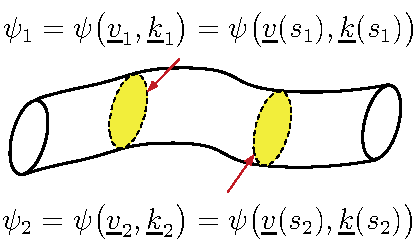
\includegraphics[width=10cm, keepaspectratio=true]{sections/cosserat_rods/images/LocalEnergy}
  \end{figure}
  
  \vspace{0.5em}
  in order to compute the strain energy $\psi$, considering relaxation of the cross section,
  we require a material model $W(.)$ from 3D elasticity, such as the Neo-Hookean solid or the Mooney-Rivlin solid  
  
%  \vspace{0.5em}
%  \textbf{strain energy of the uniformly strained rod}
%  \begin{displaymath}
%    \int_0^L \Biggl( \iint_{\Omega_0} W \bigl( \doubleunderline{F}^{\star}(X_1,X_2,s) \bigr)  \dif \Omega_0 \Biggr) \dif s =
%    \int_0^L \Biggl( \iint_{\Omega_0} W \bigl( \doubleunderline{\tilde{F}}^{\star}(X_1,X_2,s) \bigr)  \dif \Omega_0 \Biggr) \dif s =
%  \end{displaymath}
%  \begin{displaymath}
%    = \iint_{\Omega_0} W \bigl( \doubleunderline{\tilde{F}}^{\star}(X_1,X_2,s) \bigr)  \dif \Omega_0 \, \cdot L
%  \end{displaymath}
\end{frame}


%-------------------------------------------------------------------------------
\begin{frame}
  \frametitle{Deformation gradient of the star-problem}

  starting with the deformation map of the $\star$-problem
  \begin{displaymath}
    \underline{f}^{\star}(X_1,X_2,s) =
    \underline{r}^{\star}(s) + 
    \doubleunderline{R}^{\star}(s) \cdot \bigl( \underbrace{ X_{\alpha} \, \underline{e}_{\alpha} + \underline{u}^{\star}(X_1,X_2) }_{\underline{x}_0^{\star}(X_1,X_2)} \bigr)
  \end{displaymath}
  we compute its deformation gradient
  \vspace{0.3em}
  \begin{displaymath}
    \doubleunderline{F}^{\star}(X_1,X_2,s) =
  \end{displaymath}
  \begin{displaymath}
    = \underline{r}^{\star \prime}(s) \otimes \underline{e}_3 +
      \doubleunderline{R}^{\star}(s) \cdot \bigl( \underline{e}_{\alpha} \otimes \underline{e}_{\alpha} +
      \pd{\underline{u}^{\star}}{X_{\alpha}} \otimes \underline{e}_{\alpha} \bigr) +
      \doubleunderline{R}^{\star \prime}(s) \cdot \bigl( X_{\alpha} \underline{e}_{\alpha} + \underline{u}^{\star}(X_1,X_2) \bigr) \otimes \underline{e}_3 =
  \end{displaymath}
    %&\doubleunderline{R}^{\star}(s) \cdot \biggl(
    %    \doubleunderline{R}^{\star \mathrm{T}}(s) \cdot \underline{r}^{\star \prime}(s) \otimes \underline{e}_3 + 
    %    \underline{e}_{\alpha} \otimes \underline{e}_{\alpha} + 
    %    \pd{\underline{u}^{\star}}{X_{\alpha}} \otimes \underline{e}_{\alpha} +
    %    \doubleunderline{R}^{\star \mathrm{T}}(s) \cdot \doubleunderline{R}^{\star \prime}(s) \cdot \bigl( X_{\alpha} \underline{e}_{\alpha} + \underline{u}^{\star}(X_1,X_2) \bigr) \otimes \underline{e}_3 \biggr) = \\
  \begin{displaymath}
    = \doubleunderline{R}^{\star}(s) \cdot \biggl( {\color{faublue}
        \underline{v}^{\star}\cancel{(s)} \otimes \underline{e}_3 +
        \underline{e}_{\alpha} \otimes \underline{e}_{\alpha} + 
        \pd{\underline{u}^{\star}}{X_{\alpha}} \otimes \underline{e}_{\alpha} +
        \doubleunderline{K}^{\star}\cancel{(s)} \cdot \bigl( X_{\alpha} \underline{e}_{\alpha} + \underline{u}^{\star}(X_1,X_2) \bigr) \otimes \underline{e}_3 }
      \biggr) =
  \end{displaymath}
  \begin{displaymath}
    = \doubleunderline{R}^{\star}(s) \cdot \biggl( {\color{faublue}
        \underline{v}^{\star} \otimes \underline{e}_3 + 
        \underline{e}_{\alpha} \otimes \underline{e}_{\alpha} + 
        \pd{\underline{u}^{\star}}{X_{\alpha}} \otimes \underline{e}_{\alpha} +
        \underline{k}^{\star} \times \bigl( X_{\alpha} \underline{e}_{\alpha} + \underline{u}^{\star}(X_1,X_2) \bigr) \otimes \underline{e}_3 }
      \biggr) =
  \end{displaymath}
  \begin{displaymath}
    =: \doubleunderline{R}^{\star}(s) \cdot {\color{faublue} \doubleunderline{\tilde{F}}^{\star} (X_1,X_2,s) }
  \end{displaymath}
\end{frame}


%-------------------------------------------------------------------------------
\begin{frame}
  \frametitle{Warping of the cross section in the star-problem}
  without loss of generality ...
  \begin{itemize}
    \item we consider the cross section at $s=0$
    \item we prescribe $ \doubleunderline{R}^{\star}(s=0) = \doubleunderline{R}^{\star}_0 = \doubleunderline{I}$ \: (rigid body rotation)
    \item we prescribe $ \underline{r}^{\star}(s=0) = \underline{r}^{\star}_0 = \underline{0}$ \: (rigid body translation)
  \end{itemize}

  \vspace{1em}
  \textbf{minimization of energy}
  \begin{displaymath}
    \underline{u}^{\star}(X_1,X_2) =
    \argmin_{\underline{u}(X_1,X_2)} \psi \bigl( \underline{v}^{\star}, \, \underline{k}^{\star} \, ; \, \underline{u} \bigr) =
    \argmin_{\underline{u}(X_1,X_2)} \iint_{\Omega_0} W \bigl( \doubleunderline{\tilde{F}}^{\star}(X_1,X_2,s=0) \bigr)  \dif \Omega_0
  \end{displaymath}
  \begin{itemize}
    \item here $\doubleunderline{\tilde{F}}^{\star}$ is the deformation gradient we just computed \textit{but} we consider $\underline{u}(X_1,X_2)$ as a free variable, for which we optimize, i.e. $\doubleunderline{\tilde{F}}^{\star} = \doubleunderline{\tilde{F}}^{\star}(X_1,X_2,s=0 \, ; \, \underline{u})$
    \item the minimization is carried out subject to constraints: \newline
      (mass) center and orientation of the cross section must be preserved 
  \end{itemize}
  
  
\end{frame}


%-------------------------------------------------------------------------------
\begin{frame}
  \frametitle{Displacements in the star-problem (part 1)}

  \textbf{rotation / orientation of cross section}
  \begin{displaymath}
    \doubleunderline{R}^{\star \mathrm{T}}(s) \cdot \doubleunderline{R}^{\star \prime}(s) = \doubleunderline{K}^{\star} \: \text{ (const.)}
    \: \Rightarrow \:
    \doubleunderline{R}^{\star \prime}(s) = \doubleunderline{R}^{\star}(s) \cdot \doubleunderline{K}^{\star}
  \end{displaymath}
  \begin{displaymath}
    \: \Rightarrow \:
    \doubleunderline{R}^{\star}(s) = \doubleunderline{R}^{\star}_0 \cdot \exp \bigl( \doubleunderline{K}^{\star} \cdot s \bigr) = \exp \bigl( \doubleunderline{K}^{\star} \cdot s \bigr)
  \end{displaymath}
  
  \vspace{1.5em}
  \textbf{translation / displacement of cross section}
  \begin{displaymath}
    \doubleunderline{R}^{\star \mathrm{T}}(s) \cdot \underline{r}^{\star \prime}(s) = \underline{v}^{\star} \: \text{ (const.)}
    \: \Rightarrow \:
    \underline{r}^{\star \prime}(s) = \doubleunderline{R}^{\star}(s) \cdot \underline{v}^{\star} =
    \exp \bigl( \doubleunderline{K}^{\star} \cdot s \bigr) \cdot \underline{v}^{\star}
  \end{displaymath}
  \begin{displaymath}
    \underline{r}^{\star}(s) = \cancel{ \underline{r}^{\star}_0 } + \Biggl( \int_0^s \exp \bigl( \doubleunderline{K}^{\star} \cdot l \bigr) \dif l \Biggr) \cdot \underline{v}^{\star}
  \end{displaymath}
  
\end{frame}


%-------------------------------------------------------------------------------
\begin{frame}
  \frametitle{Displacements in the star-problem (part 2)}
  
  \textbf{decomposition of $\underline{v}^{\star}$} \newline
  we split $\underline{v}^{\star}$ in a part that is parallel to $\underline{k}^{\star}$ and a part that is perpendicular to $\underline{k}^{\star}$
  \begin{displaymath}
    \underline{v}^{\star} = \bigl( \cos(\phi) \cdot \underline{\hat{k}} + \sin(\phi) \cdot \underline{\hat{k}}^{\perp} \bigr) \cdot \, \norm[1]{\underline{v}^{\star}}
  \end{displaymath}
  \begin{itemize}
    \item $\phi$ is the angle between $\underline{v}^{\star}$ and $\underline{k}^{\star}$, i.e. $\phi = \arcsin \Bigl( \frac{\underline{v}^{\star} \cdot \underline{k}^{\star}}{\norm[0]{\underline{v}^{\star}} \, \cdot \: \norm[0]{\underline{k}^{\star}}} \Bigr)$
    \item $\underline{\hat{k}}$ is the unit vector along $\underline{k}^{\star}$, i.e. $\underline{\hat{k}} = \frac{\underline{k}^{\star}}{\norm[0]{\underline{k}^{\star}}}$
    \item $\underline{\hat{k}}^{\perp}$ is a unit vector perpendicular to $\underline{\hat{k}}$
  \end{itemize}
  
  \vspace{0.5em}
  \textbf{translation / displacement of cross section (revisited)}
  \begin{displaymath}
    \underline{r}^{\star}(s) = \Biggl( \underbrace{\cos(\phi) \cdot \int_0^s \overbrace{\exp \bigl( \doubleunderline{K}^{\star} \cdot l \bigr) \cdot \underline{\hat{k}} }^{\underline{\hat{k}}} \, \dif l}_{\text{straight line along }\underline{\hat{k}}}  + \underbrace{ \sin(\phi) \cdot \int_0^s \exp \bigl( \doubleunderline{K}^{\star} \cdot l \bigr) \cdot \underline{\hat{k}}^{\perp} \dif l}_{\text{circle with normal along }\underline{\hat{k}}} \Biggr) \cdot \norm[1]{\underline{v}^{\star}}
  \end{displaymath}
  
\end{frame}


%-------------------------------------------------------------------------------
\begin{frame}
  \frametitle{The centerline turns into a helix}
  \vspace{-1em}
  \begin{displaymath}
    \underline{r}^{\star}(s) = \Biggl( \cos(\phi) \cdot \underline{\hat{k}} \cdot s + \sin(\phi) \cdot \int_0^s \exp \bigl( \doubleunderline{K}^{\star} \cdot l \bigr) \cdot \underline{\hat{k}}^{\perp} \dif l \Biggr) \cdot \norm[1]{\underline{v}^{\star}}
  \end{displaymath}
  \vspace{-0.8em}
  \begin{figure}
    \centering
    \includegraphics[width=14cm, keepaspectratio=true]{sections/cosserat_rods/images/HelixContinuum}
  \end{figure}
\end{frame}


%-------------------------------------------------------------------------------
\begin{frame}
  \frametitle{Helix equation}

  rewriting the equation we get ...  %TODO integration of matrix exponential: K is singular!?
  \begin{displaymath}
    \underline{r}^{\star}(s) = \norm[1]{\underline{v}^{\star}} \cdot \Biggl( \cos(\phi) \cdot \underline{\hat{k}} \cdot s + \sin(\phi) \cdot \frac{1}{\norm[1]{\underline{k}^{\star}}} \cdot \biggl( \doubleunderline{I} - \exp \bigl( \doubleunderline{K}^{\star} \cdot s \bigr) \biggr) \cdot \underline{\hat{k}} \times \underline{\hat{k}}^{\perp} \Biggr)
  \end{displaymath}
  
  \vspace{0.5em}
  we introduce the abbreviations
  \begin{itemize}
    \item $\tau = \norm[1]{\underline{v}^{\star}} \cdot \cos(\phi)$
    \item $\underline{x}_f = \frac{\sin(\phi) \cdot \underline{\hat{k}} \times \underline{\hat{k}}^{\perp}}{\norm[0]{\underline{k}^{\star}}} = \frac{\underline{v}^{\star} \times \underline{k}^{\star}}{\norm[0]{\underline{k}^{\star}}^2}$ (fixed point of the helix)
  \end{itemize}
  
  \vspace{0.7em}
  and get ...
  \begin{displaymath}
    \underline{r}^{\star}(s) = s \cdot \tau \cdot \underline{\hat{k}} + \biggl( \doubleunderline{I} - \exp \bigl( \doubleunderline{K}^{\star} \cdot s \bigr) \biggr) \cdot \underline{x}_f =
    s \cdot \tau \cdot \underline{\hat{k}} + \underbrace{ \underline{x}_f + \doubleunderline{R}^{\star}(s) \cdot \bigl( \underline{r}^{\star}_0 - \underline{x}_f \bigr) }_{\text{rotation of the origin about }\underline{x}_f}
  \end{displaymath}
  
  \vspace{0.3em}
  \textbf{examples}
  \begin{itemize}
    \item $\underline{v}^{\star} \parallel \underline{k}^{\star}$ : 
      centerline degenerates into a straight line (e.g. combined extension \& torsion)
    \item $\underline{v}^{\star} \perp \underline{k}^{\star}$ : 
      centerline degenerates into a circle (e.g. pure bending)
  \end{itemize}
\end{frame}


%-------------------------------------------------------------------------------
\begin{frame}
  \frametitle{Helix}

  \vspace{-1em}
  \begin{multicols}{2}
    \noindent
    
    \begin{displaymath}
      \begin{alignedat}{1}
        &\underline{r}^{\star}(s) = \\
        &s \cdot \tau \cdot \underline{\hat{k}} +
        \underline{x}_f + \exp \bigl( \doubleunderline{K}^{\star} \cdot s \bigr) \cdot \bigl( \underline{r}^{\star}_0 - \underline{x}_f \bigr)  
      \end{alignedat}
    \end{displaymath}

    \begin{figure}
      \centering
      \includegraphics[width=11cm, keepaspectratio=true]{sections/cosserat_rods/images/HelixContinuum}
    \end{figure}
    
    \textbf{pitch} \\
    for one full turn of the helix we have
    \begin{displaymath}
      \norm[1]{\underline{k}^{\star}} \cdot \overset{\circ}{s} \overset{!}{=} 2 \cdot \pi
    \end{displaymath}
    
    plugging $\overset{\circ}{s}$ into the part of the helix equation that generates the axial motion we obtain the pitch of the helix as
    \begin{displaymath}
      \overset{\circ}{s} \cdot \tau = \frac{2 \, \pi}{\norm[1]{\underline{k}^{\star}}} \cdot \norm[1]{\underline{v}^{\star}} \cdot \cos(\phi)
    \end{displaymath}
    
    \vspace{1em}
    \textbf{radius}
    \begin{displaymath}
      \norm[1]{\underline{r}^{\star}_0 - \underline{x}_f} =
      \norm[1]{\underline{x}_f}
    \end{displaymath}
    
  \end{multicols}

\end{frame}






%-------------------------------------------------------------------------------
\begin{frame}
  \frametitle{Deformation map and deformation gradient of the star-problem}

  we rewrite the \textbf{deformation map} of the $\star$-problem, using the helix equation ... 
  \begin{displaymath}
    \underline{f}^{\star}(X_1,X_2,s) =
    \underline{r}^{\star}(s) + 
    \doubleunderline{R}^{\star}(s) \cdot \bigl( {\color{faublue} X_{\alpha} \, \underline{e}_{\alpha} + \underline{u}^{\star}(X_1,X_2)} \bigr) = 
    \underline{r}^{\star}(s) + 
    \doubleunderline{R}^{\star}(s) \cdot {\color{faublue} \underline{x}^{\star}_0(X_1,X_2)} =
  \end{displaymath}
  \begin{displaymath}
    = s \cdot \tau \cdot \underline{\hat{k}} + \underline{x}_f + \doubleunderline{R}^{\star}(s) \cdot \bigl( {\color{faublue} \underline{x}^{\star}_0(X_1,X_2)} - \underline{x}_f \bigr)
  \end{displaymath}
  $\rightarrow$ rotating $\underline{r}^{\star} = \underline{0}$ about $\underline{x}_f$ creates centerline ; rotating $\underline{x}^{\star}_0$ about $\underline{x}_f$ creates entire rod
  
  \vspace{1.5em}
  and then we compute its \textbf{deformation gradient} ...
  \begin{displaymath}
    \doubleunderline{F}^{\star}(X_1,X_2,s) =
    \underline{r}^{\star \prime}(s) \otimes \underline{e}_3 +
    \doubleunderline{R}^{\star \prime}(s) \cdot \underline{x}_0^{\star}(X_1,X_2) \otimes \underline{e}_3 +
    \doubleunderline{R}^{\star}(s) \cdot \pd{\underline{x}_0^{\star}}{X_{\alpha}} \otimes \underline{e}_{\alpha} =
  \end{displaymath}
  \begin{displaymath}
  = \doubleunderline{R}^{\star}(s) \cdot \Bigl(
      \doubleunderline{R}^{\star \mathrm{T}}(s) \cdot \underline{r}^{\star \prime}(s) \otimes \underline{e}_3 +
      \doubleunderline{R}^{\star \mathrm{T}}(s) \cdot \doubleunderline{R}^{\star \prime}(s) \cdot \underline{x}_0^{\star}(X_1,X_2) \otimes \underline{e}_3 +
      \pd{\underline{x}_0^{\star}}{X_{\alpha}} \otimes \underline{e}_{\alpha}
    \Bigr) =
  \end{displaymath}
  \begin{displaymath}
    = \doubleunderline{R}^{\star}(s) \cdot \Bigl(
      \underline{v}^{\star} \otimes \underline{e}_3 +
      \bigl( \underline{k}^{\star} \times \underline{x}_0^{\star}(X_1,X_2) \bigr) \otimes \underline{e}_3 +
      \pd{\underline{x}_0^{\star}}{X_{\alpha}} \otimes \underline{e}_{\alpha}
    \Bigr)
  \end{displaymath}

\end{frame}


%-------------------------------------------------------------------------------
\begin{frame}
  \frametitle{2D minimization problem (part 1)}

%  \begin{displaymath} %arg min version
%    \underline{u}^{\star}(X_1,X_2) =
%    \argmin_{\underline{u}} \psi \bigl( \underline{v}^{\star}, \, \underline{k}^{\star} \, ; \, \underline{u} \bigr) =
%    \argmin_{\underline{u}} \iint_{\Omega_0} W \bigl( \doubleunderline{\tilde{F}}^{\star}(X_1,X_2,s=0) \bigr)  \dif \Omega_0
%  \end{displaymath}
  \begin{displaymath}
    \min_{\underline{x}_0^{\star}} \iint_{\Omega_0} W \bigl( \doubleunderline{\tilde{F}}^{\star}(X_1,X_2,s=0) \bigr)  \dif \Omega_0
  \end{displaymath}
  such that ... \newline
  $\circ$ the center(line) remains at the origin or more precisely that the mass center of the cross section remains in the origin, i.e.
  \begin{displaymath}
    \iint_{\Omega_0} \rho_0 \cdot \underline{x}_0^{\star} \, \dif \Omega_0 = \underline{0}
  \end{displaymath}
  $\circ$ and such that orientation of the cross section remains in the $\underline{e}_1$-$\underline{e}_2$-plane or more precisely that the principal axis of the inertia tensor remains aligned with the $\underline{e}_3$-axis ; this is the same as saying that the mixed moments of inertia must vanish
  \begin{displaymath}
    \iint_{\Omega_0} \underbrace{ \rho_0 \cdot 
    \begin{bmatrix}
      x_2 \cdot x_3 \\
      x_1 \cdot x_3 \\
      x_1 \cdot x_2 
    \end{bmatrix} }_{=: \underline{M}}
    \dif \Omega_0 = \underline{0}
  \end{displaymath}
  with $x_i$ the components of $\underline{x}_0^{\star}$
\end{frame}


%-------------------------------------------------------------------------------
\begin{frame}
  \frametitle{2D minimization problem (part 2)}

  \textbf{minimization problem with augmented Langrangian}
  \begin{displaymath}
    \min_{\underline{x}_0^{\star},\underline{\lambda},\underline{\mu}} \iint_{\Omega_0} \Bigl( W \bigl( \doubleunderline{\tilde{F}}^{\star}(X_1,X_2,s=0) \bigr) + \underline{\lambda} \cdot \rho_0 \cdot \underline{x}_0^{\star} + \underline{\mu} \cdot \underline{M} \Bigr) \dif \Omega_0
  \end{displaymath}
  
  \vspace{0.5em}
  \textbf{perturbed version of $\underline{x}_0^{\star}$}
  \begin{displaymath}
    \underline{x}_0^{\epsilon}(X_1,X_2) = \underline{x}_0^{\star}(X_1,X_2) + \epsilon \cdot \delta \underline{x}_0^{\star}(X_1,X_2)
  \end{displaymath}
  
  \vspace{0.5em}
  \textbf{perturbed version of the cross section energy}
  \begin{displaymath}
    \psi_{\epsilon} = 
    \iint_{\Omega_0} \Bigl(
      W \bigl( \doubleunderline{\tilde{F}}^{\epsilon}(X_1,X_2,s=0) \bigr) + 
      \underline{\lambda} \cdot \rho_0 \cdot \underline{x}_0^{\epsilon}(X_1,X_2) +
      \underline{\mu} \cdot \underline{M}^{\epsilon}(X_1,X_2)
    \Bigr) \dif \Omega_0
  \end{displaymath}
  
  \vspace{0.5em}
  \textbf{first variation of the cross section energy}
  \begin{displaymath}
    \delta \psi = \od{\psi_{\epsilon}}{\epsilon} \sVert[3]_{\epsilon=0} =
    \iint_{\Omega_0} \Bigl(
      \underbrace{\pd{W}{\doubleunderline{F}}}_{\doubleunderline{P}} \colon \od{\doubleunderline{\tilde{F}}^{\epsilon}}{\epsilon} \sVert[3]_{\epsilon=0} +
      \underline{\lambda} \cdot \rho_0 \cdot \od{\underline{x}_0^{\epsilon}}{\epsilon} \sVert[3]_{\epsilon=0} +
      \underline{\mu} \cdot \od{\underline{M}^{\epsilon}}{\epsilon} \sVert[3]_{\epsilon=0}
    \Bigr) \dif \Omega_0
  \end{displaymath}
  
\end{frame}


%-------------------------------------------------------------------------------
\begin{frame}
  \frametitle{2D minimization problem (part 3)}

  from
  \begin{displaymath}
    \doubleunderline{F}^{\epsilon}(X_1,X_2,s) =
    \doubleunderline{R}^{\star}(s) \cdot \Bigl(
      \underline{v}^{\star} \otimes \underline{e}_3 +
      \bigl( \underline{k}^{\star} \times \underline{x}_0^{\epsilon}(X_1,X_2) \bigr) \otimes \underline{e}_3 +
      \pd{\underline{x}_0^{\epsilon}}{X_{\alpha}} \otimes \underline{e}_{\alpha}
    \Bigr)  
  \end{displaymath}
  it follows that
  \begin{displaymath}
    \od{\doubleunderline{\tilde{F}}^{\epsilon}}{\epsilon} \sVert[3]_{\epsilon=0} =
    \bigl( \underline{k}^{\star} \times \delta \underline{x}_0^{\star}(X_1,X_2) \bigr) \otimes \underline{e}_3 +
    \pd{\delta \underline{x}_0^{\star}}{X_{\alpha}} \otimes \underline{e}_{\alpha}
  \end{displaymath}
  
  \vspace{1em}
  and from
  \begin{displaymath}
    \underline{M}^{\epsilon} =
    \rho_0 \cdot 
    \begin{bmatrix}
      x_2^{\epsilon} \cdot x_3^{\epsilon} \\
      x_1^{\epsilon} \cdot x_3^{\epsilon} \\
      x_1^{\epsilon} \cdot x_2^{\epsilon} 
    \end{bmatrix} = 
    \rho_0 \cdot
    \begin{bmatrix}
      (x_2 + \epsilon \cdot \delta x_2) \cdot (x_3 + \epsilon \cdot \delta x_3) \\
      (x_1 + \epsilon \cdot \delta x_1) \cdot (x_3 + \epsilon \cdot \delta x_3) \\
      (x_1 + \epsilon \cdot \delta x_1) \cdot (x_2 + \epsilon \cdot \delta x_2) 
    \end{bmatrix}
  \end{displaymath}
  it follows that
  \begin{displaymath}
    \od{\underline{M}^{\epsilon}}{\epsilon} \sVert[3]_{\epsilon=0} =
    \rho_0 \cdot 
    \begin{bmatrix}
      x_2 \cdot \delta x_3 + x_3 \cdot \delta x_2\\
      x_1 \cdot \delta x_3 + x_3 \cdot \delta x_1\\
      x_1 \cdot \delta x_2 + x_2 \cdot \delta x_1
    \end{bmatrix} =
    \underbrace{ \rho_0 \cdot
    \begin{bmatrix}
      0 & x_3 & x_2 \\
      x_3 & 0 & x_1 \\
      x_2 & x_1 & 0
    \end{bmatrix} }_{=: \doubleunderline{M}(X_1,X_2)} \cdot \delta \underline{x}_0^{\star}(X_1,X_2)
  \end{displaymath}
  
\end{frame}


%-------------------------------------------------------------------------------
\begin{frame}
  \frametitle{2D minimization problem (part 4)}

  note that
  \begin{displaymath}
    \doubleunderline{P} \colon \bigl( \underline{a} \otimes \underline{b} \bigr) \: \hat{=} \: P_{ij} \, a_i \, b_j = P_{ij} \, b_j \, a_i \: \hat{=} \: \bigl( \doubleunderline{P} \cdot \underline{b} \bigr) \cdot \underline{a}
  \end{displaymath}
  and that
  \begin{displaymath}
    \underline{a} \cdot \bigl( \underline{b} \times \underline{c} \bigr) =
    \underline{b} \cdot \bigl( \underline{c} \times \underline{a} \bigr) =
    \underline{c} \cdot \bigl( \underline{a} \times \underline{b} \bigr)
  \end{displaymath}

  \vspace{1em}
  \textbf{first variation of the cross section energy}
  \begin{displaymath}
    \delta \psi = 
    \iint_{\Omega_0} \Biggl(
      \doubleunderline{P} \colon \Bigl(
        \bigl( \underline{k}^{\star} \times \delta \underline{x}_0^{\star} \bigr) \otimes \underline{e}_3 +
        \pd{\delta \underline{x}_0^{\star}}{X_{\alpha}} \otimes \underline{e}_{\alpha}
      \Bigr) +
      \underline{\lambda} \cdot \biggl( \rho_0 \cdot \delta \underline{x}_0^{\star} \biggr) +
      \underline{\mu} \cdot \biggl( \doubleunderline{M} \cdot \delta \underline{x}_0^{\star} \biggr)
    \Biggr) \dif \Omega_0 = 
  \end{displaymath}
  \begin{displaymath}
    = \iint_{\Omega_0} \Biggl(
      \bigl( \doubleunderline{P} \cdot \underline{e}_3 \bigr) \cdot \bigl( \underline{k}^{\star} \times \delta \underline{x}_0^{\star} \bigr) +
      \overbrace{
      \bigl( \doubleunderline{P} \cdot \underline{e}_{\alpha} \bigr) \cdot \pd{\delta \underline{x}_0^{\star}}{X_{\alpha}} }^{\rightarrow \text{IBP}} +
      \bigl(
        \rho_0 \cdot \underline{\lambda} +
        \doubleunderline{M} \cdot \underline{\mu}
      \bigr) \cdot \delta \underline{x}_0^{\star}
    \Biggr) \dif X_1 \, \dif X_2 =
  \end{displaymath}
  \begin{displaymath}
    = \iint_{\Omega_0} \Biggl(
      \biggl( \bigl( \doubleunderline{P} \cdot \underline{e}_3 \bigr) \times \underline{k}^{\star} \biggr) \cdot \delta \underline{x}_0^{\star} +
      \pd{}{X_{\alpha}} \biggl( \bigl( \doubleunderline{P} \cdot \underline{e}_{\alpha} \bigr) \cdot \delta \underline{x}_0^{\star} \biggr) -
      \pd{}{X_{\alpha}} \biggl( \doubleunderline{P} \cdot \underline{e}_{\alpha} \biggr) \cdot \delta \underline{x}_0^{\star} \: +
  \end{displaymath}
  \begin{displaymath}
      + \bigl(
        \rho_0 \cdot \underline{\lambda} +
        \doubleunderline{M} \cdot \underline{\mu}
      \bigr) \cdot \delta \underline{x}_0^{\star}
    \Biggr) \dif \Omega_0 = \dots
  \end{displaymath}
  
\end{frame}


%-------------------------------------------------------------------------------
\begin{frame}
  \frametitle{2D minimization problem (part 5)}
  \vspace{-1em}
  \begin{displaymath}
    \delta \psi = 
    \iint_{\Omega_0} \Biggl(
      \biggl( \bigl( \doubleunderline{P} \cdot \underline{e}_3 \bigr) \times \underline{k}^{\star} \biggr) \cdot \delta \underline{x}_0^{\star} +
      \pd{}{X_{\alpha}} \biggl( \bigl( \doubleunderline{P} \cdot \underline{e}_{\alpha} \bigr) \cdot \delta \underline{x}_0^{\star} \biggr) -
      \pd{}{X_{\alpha}} \biggl( \doubleunderline{P} \cdot \underline{e}_{\alpha} \biggr) \cdot \delta \underline{x}_0^{\star} \: +
  \end{displaymath}
  \begin{displaymath}
      + \bigl(
        \rho_0 \cdot \underline{\lambda} +
        \doubleunderline{M} \cdot \underline{\mu}
      \bigr) \cdot \delta \underline{x}_0^{\star}
    \Biggr) \dif \Omega_0 =
  \end{displaymath}
  \begin{displaymath}
    = \iint_{\Omega_0} - \Biggl(
      \pd{}{X_{\alpha}} \biggl( \doubleunderline{P} \cdot \underline{e}_{\alpha} \biggr) +
      \underline{k}^{\star} \times \bigl( \doubleunderline{P} \cdot \underline{e}_3 \bigr) -
      \bigl(
        \rho_0 \cdot \underline{\lambda} +
        \doubleunderline{M} \cdot \underline{\mu}
      \bigr)
    \Biggr) \cdot \delta \underline{x}_0^{\star} \, \dif \Omega_0 \: +
  \end{displaymath}
  \begin{displaymath}
    + \iint_{\Omega_0}
      \pd{}{X_{\alpha}} \biggl( \bigl( \doubleunderline{P} \cdot \underline{e}_{\alpha} \bigr) \cdot \delta \underline{x}_0^{\star} \biggr)
    \dif \Omega_0
  \end{displaymath}
  
  
\end{frame}


%-------------------------------------------------------------------------------
\begin{frame}
  \frametitle{2D minimization problem (part 6)}

  for the second integral we can use the divergence theorem ...
  \begin{displaymath}
    \iint_{\Omega_0}
      \pd{}{X_{\alpha}} \biggl( \bigl( \doubleunderline{P} \cdot \underline{e}_{\alpha} \bigr) \cdot \delta \underline{x}_0^{\star} \biggr)
    \dif \Omega_0 =
    \iint_{\Omega_0}
      \pd{}{X_{\alpha}} \biggl( \bigl( \doubleunderline{P}^{\mathrm{T}} \cdot \delta \underline{x}_0^{\star} \bigr) \cdot \underline{e}_{\alpha} \biggr)
    \dif \Omega_0 =
  \end{displaymath}
  \begin{displaymath}
    = \iint_{\Omega_0}
      \underline{\nabla} \cdot \bigl( \doubleunderline{P}^{\mathrm{T}} \cdot \delta \underline{x}_0^{\star} \bigr)
    \dif \Omega_0 =
    \int_{\partial \Omega_0}
      \bigl( \doubleunderline{P}^{\mathrm{T}} \cdot \delta \underline{x}_0^{\star} \bigr) \cdot \underline{n}_0 \,
    \dif l =
    \int_{\partial \Omega_0}
      \bigl( \doubleunderline{P} \cdot \underline{n}_0 \bigr) \cdot \delta \underline{x}_0^{\star} \,
    \dif l
  \end{displaymath}
  with $\underline{n}_0$ the unit normal of the cross section boundary
  
  \vspace{1em}
  setting $\delta \psi = 0$ gives us the \textbf{Euler-Lagrange equations} of the $\star$-problem
  \begin{displaymath}
    \underline{\nabla}_{\alpha} \cdot \doubleunderline{P} +
    \underline{k}^{\star} \times \bigl( \doubleunderline{P} \cdot \underline{e}_3 \bigr) =
    \rho_0 \cdot \underline{\lambda} +
    \doubleunderline{M} \cdot \underline{\mu}
    \: \text{ in } \Omega_0    
  \end{displaymath}
  \begin{displaymath}
    \doubleunderline{P} \cdot \underline{n}_0 = \underline{0}
    \: \text{ on } \partial \Omega_0
    \: \text{ (traction free boundary condition)}
  \end{displaymath}
  
  \vspace{1em}
  %TODO why constraints again? (augmented Langrangian)
  % perturbations del_lambda, del_mu
  % variations for del_lambda, del_mu
  % set these also to zero
  % this ist equal to saying: plus the constraints

  % P = ConstitutiveLaw(strains(x-star), x-star)
  together with the constraints
  \begin{displaymath}
    \iint_{\Omega_0} \rho_0 \cdot \underline{x}_0^{\star} \, \dif \Omega_0 = \underline{0}
    \quad \text{ and } \quad
    \iint_{\Omega_0} \underline{M} \dif \Omega_0 = \underline{0}
  \end{displaymath}
  the Euler-Lagrange equations are the (necessary) conditions for a minimum of the cross section energy ; $\underline{x}_0^{\star}(X_1,X_2)$, $\underline{\lambda}$ and $\underline{\mu}$ are the unknowns of the problem
\end{frame}



%===============================================================================
\subsection{Modeling of 1D nanostructures}

%-------------------------------------------------------------------------------
\begin{frame}
  \frametitle{Recap}

  \textbf{strain energy density function} (per unit of undeformed length)
  \begin{displaymath}
    \psi \bigl( \underline{v} , \, \underline{k} \, ; \, \underline{u}(\underline{v} , \, \underline{k}) \bigr) =
    \iint_{\Omega_0} W \bigl( \doubleunderline{F} \bigr) \dif \Omega_0
  \end{displaymath}
  
  \textbf{deformation gradient} of the $\star$-problem
  \begin{displaymath}
    \doubleunderline{F}^{\star}(X_1,X_2,s) =
    \doubleunderline{R}^{\star}(s) \cdot \Bigl(
      \underline{v}^{\star} \otimes \underline{e}_3 +
      \bigl( \underline{k}^{\star} \times \underbrace{ \underline{x}_0^{\star}(X_1,X_2) }_{\text{warping function}} \bigr) \otimes \underline{e}_3 +
      \pd{\underline{x}_0^{\star}}{X_{\alpha}} \otimes \underline{e}_{\alpha}
    \Bigr)
  \end{displaymath}
  
  in order to find $\underline{x}_0^{\star}(X_1,X_2)$ we must find a solution to the
  \textbf{Euler-Lagrange equations} of the $\star$-problem
  \begin{displaymath}
    \underline{\nabla}_{\alpha} \cdot \doubleunderline{P} +
    \underline{k}^{\star} \times \bigl( \doubleunderline{P} \cdot \underline{e}_3 \bigr) =
    \rho_0 \cdot \underline{\lambda} +
    \doubleunderline{M} \cdot \underline{\mu}
    \: \text{ in } \Omega_0    
  \end{displaymath}
  \begin{displaymath}
    \doubleunderline{P} \cdot \underline{n}_0 = \underline{0}
    \: \text{ on } \partial \Omega_0
    \: \text{ (traction free boundary condition)}
  \end{displaymath}
  
  \vspace{0.5em}
  that also respects the \textbf{kinematic constraints}
  \begin{displaymath}
    \iint_{\Omega_0} \rho_0 \cdot \underline{x}_0^{\star} \, \dif \Omega_0 = \underline{0}
    \quad \text{ and } \quad
    \iint_{\Omega_0} \underline{M} \dif \Omega_0 = \underline{0}
  \end{displaymath}

\end{frame}


%-------------------------------------------------------------------------------
\begin{frame}
  \frametitle{Modeling of continuum and nanorods using molecular approaches}

  \begin{itemize}
    \item what is the form of $W \bigl( \doubleunderline{F} \bigr)$ ?
      \begin{itemize}
        \item either obtain it from experiments ...
        \item or use theory $\rightarrow$ molecular approach called \textit{Cauchy Born rule}
      \end{itemize}
    \item if the radius of the rod is at the nanoscale surface effects become also important, i.e.
      \begin{displaymath}
        \psi \bigl( \underline{v} , \, \underline{k} \bigr) =
        \underbrace{ \iint_{\Omega_0} W \bigl( \doubleunderline{F} \bigr) \dif \Omega_0 }_{\text{bulk energy}} +
        \underbrace{ \int_{\partial \Omega_0} \psi^S \bigl( \doubleunderline{E}^S \bigr) \dif l }_{\text{surface energy}}
      \end{displaymath}
      \null \quad $\rightarrow$ extension of the approach called \textit{Surface Cauchy Born rule}
    \item hollow tube at nanoscale (SWCNT = single wall carbon nanotube)
      \begin{itemize}
        \item can not be thought of as a 3D continuum anymore!
        \item $\psi \bigl( \underline{v} , \, \underline{k} \bigr) \rightarrow$ direct approach called \textit{Helical Cauchy Born rule}
      \end{itemize}
  \end{itemize}
\end{frame}


%-------------------------------------------------------------------------------
\begin{frame}
  \frametitle{Arrangement of atoms in crystalline materials (part 1)}
  
  crystals have a regular arrangement of atoms: translational periodicity
  \begin{multicols}{2}
    \noindent
    consider for example a simple 2D crystal:
    
    \vspace{0.3em}
    \begin{figure}
      \centering
      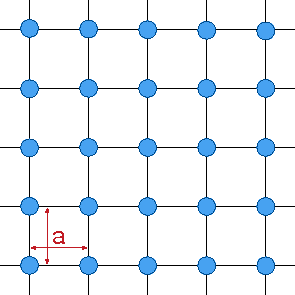
\includegraphics[width=8cm, keepaspectratio=true]{sections/cosserat_rods/images/CrystalLattice2D}
    \end{figure}
    
    to generate any crystal we need
    \begin{itemize}
      \item lattice vectors: $\bigl( \underline{A}_1, \, \underline{A}_2 , \, \underline{A}_3 \bigr)$
      \item basis atoms: $\underline{X}_{0,j}$ with $j = 1, \dots , M$
        \begin{itemize}
          \item $M$ the number of atoms per unit cell ;
          \item the zero index indicates the unit cell
        \end{itemize}
    \end{itemize}
    
    \vspace{0.8em}
    in this 2D example we have
    \begin{itemize}
      \item $\bigl( \underline{A}_1, \, \underline{A}_2 \bigr) = \bigl( a \cdot \underline{e}_1, \, a \cdot \underline{e}_2 \bigr)$
      \item $\underline{X}_{\underline{0},1} = \bigl( 0 , \, 0 \bigr)$ \: ; $M=1$
    \end{itemize}
    
  \end{multicols}
  

\end{frame}


%-------------------------------------------------------------------------------
\begin{frame}
  \frametitle{Arrangement of atoms in crystalline materials (part 2)}

  \textbf{generators of a crystal}  \begin{displaymath}
    \underline{X}_{(n_1,n_2,n_3,j)} =
    n_i \cdot \underline{A}_i + \bigl( \underline{X}_j \bigr)_{j=1,\dots,M} =
    \underbrace{ n_1 \cdot \underline{A}_1 + n_2 \cdot \underline{A}_2 + n_3 \cdot \underline{A}_3 }_{\text{generates lattice}} + \underbrace{ \bigl( \underline{X}_j \bigr)_{j=1,\dots,M} }_{\text{puts atoms on lattice}}
  \end{displaymath}
    
  \vspace{-0.3em}
  $n_1, \, n_2, \, n_3 \in \mathbb{Z}$ gives the translation of the unit cell and \newline
  $j=1,\dots,M$ represents the different atoms that are present within the unit cell
  
  
  \vspace{1em}
  \textbf{2D example from last slide}
  \begin{multicols}{2}
    \noindent
    \begin{figure}
      \centering
      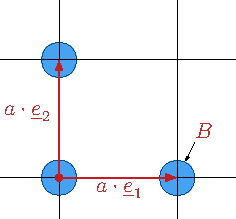
\includegraphics[width=8cm, keepaspectratio=true]{sections/cosserat_rods/images/CrystalLattice2DGeneratingFunction}
    \end{figure}
  
    atom $B$ is generated by
    \begin{displaymath}
      \underline{X}_B =
      \underline{X}_{(1,0,1)} =
    \end{displaymath}
    \begin{displaymath}
      = \underbrace{1}_{n_1} \cdot \underbrace{(a \cdot \underline{e}_1)}_{\underline{A}_1} +
      \underbrace{0}_{n_2} \cdot \underbrace{(a \cdot \underline{e}_2)}_{\underline{A}_2} +
      0 \cdot \underline{e}_1 +
      0 \cdot \underline{e}_2
    \end{displaymath}
  \end{multicols}

\end{frame}

%-------------------------------------------------------------------------------
\begin{frame}
  \frametitle{Arrangement of atoms in crystalline materials (part 3)}

  \textbf{another example: BCC crystal} (body centered cubic)
  \begin{multicols}{2}
    \noindent
    unit cell with two atoms
    
    \begin{figure}
      \centering
      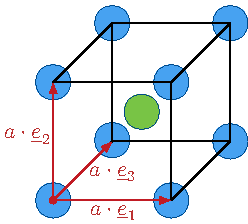
\includegraphics[width=8cm, keepaspectratio=true]{sections/cosserat_rods/images/CrystalLatticeBBC}
    \end{figure}
    
    the 7 blue atoms, that are not at the origin, actually belong to the neighboring unit cells!
  
    \vspace{2em}
    \begin{itemize}
      \item lattice vectors: $\bigl( \underline{A}_1, \, \underline{A}_2, \, \underline{A}_3 \bigr) = \bigl( a \cdot \underline{e}_1, \, a \cdot \underline{e}_2 , \, a \cdot \underline{e}_3 \bigr)$
      \item basis atoms: \newline
        $\underline{X}_{\underline{0},1} = \bigl( 0 , \, 0 , \, 0 \bigr)$
        $\underline{X}_{\underline{0},2} = \frac{a}{2} \cdot \bigl( \underline{e}_1 + \underline{e}_2 + \underline{e}_3 \bigr)$ \: ; $M=2$
    \end{itemize}
  \end{multicols}
\end{frame}


%-------------------------------------------------------------------------------
\begin{frame}
  \frametitle{Cauchy Born rule (part 1)}
  
  \begin{itemize}
    \item at the continuum level : straining a rod
    \item at the molecular level : the atoms are moving
    \item the movement of atoms is determined by the bond energy between the atoms
    \item assumption: periodicity is maintained by slowly varying deformations
  \end{itemize}
  
  \begin{figure}
    \centering
    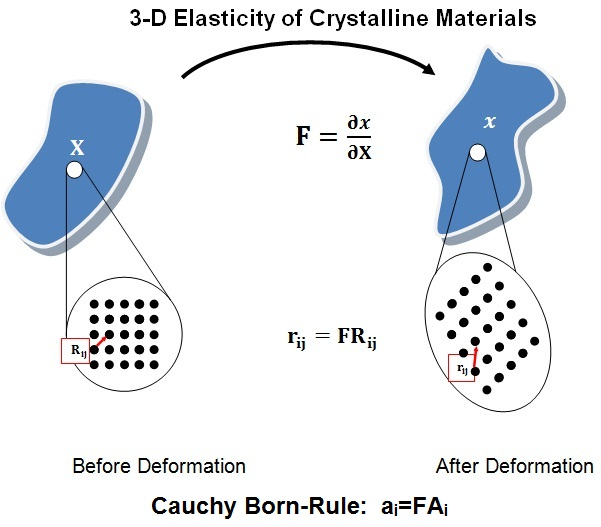
\includegraphics[width=11cm, keepaspectratio=true]{sections/cosserat_rods/images/DeformedCrystalLatticePrakhar}
    %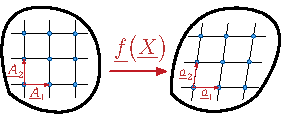
\includegraphics[width=18cm, keepaspectratio=true]{sections/cosserat_rods/images/DeformedCrystalLattice}
  \end{figure}
%  with
%  \begin{displaymath}
%    \underline{a}_1 = \doubleunderline{F} \cdot \underline{A}_1
%    \quad \text{ and } \quad
%    \underline{a}_2 = \doubleunderline{F} \cdot \underline{A}_2
%  \end{displaymath}

\end{frame}


%-------------------------------------------------------------------------------
\begin{frame}
  \frametitle{Cauchy Born rule (part 2)}
  
  as an example consider the homogeneous deformation map
  \begin{displaymath}
    \begin{alignedat}{1}
      x_1 &= X_1 \\
      x_2 &= X_2 \\
      x_3 &= \lambda \cdot X_3 \quad \Rightarrow \quad \underline{a}_3 = \lambda \cdot \underline{A}_3
    \end{alignedat}
  \end{displaymath}
  if the continuum deformation map is also valid at the atomic level, we have $\underline{a}_3 = \lambda \cdot \underline{A}_3$ \newline
  or more generally the Cauchy Born rule
  \begin{displaymath}
    \underline{a}_i = \doubleunderline{F} \cdot \underline{A}_i
  \end{displaymath}
  \begin{itemize}
    \item bridges the continuum and the atomistic viewpoint
    \item the crystal lattice deforms like the continuum
    \item the positions of the atoms are still unknown \newline
      (they are not dictated by the macroscopic deformation gradient)
  \end{itemize}
  
  \vspace{0.7em}
  the position of \textit{any} atom in the deformed configuration is given by
  \begin{displaymath}
    \underline{x}_{(n_1,n_2,n_3,j)} =
    n_i \cdot \doubleunderline{F} \cdot \underline{A}_i + \underline{x}_{\underline{0},j}
  \end{displaymath}
  where $\underline{x}_{\underline{0},j}$ are the positions of the basis atoms within the unit cell \newline %F is non-homogeneous then every unit cell has different x_j ; that's why deformation must be slowly varying
  $\rightarrow$ unknowns : can be determined by minimizing the energy of the unit cell
  
\end{frame}


%-------------------------------------------------------------------------------
\begin{frame}
  \frametitle{Minimizing the energy of the unit cell (part 1)}

  \textbf{average strain energy density of the unit cell}
  \begin{displaymath}
    W \bigl( \doubleunderline{F} \bigr) =
    \min_{(\underline{x}_{\underline{0},1},\dots,\underline{x}_{\underline{0},M})} \frac{E \bigl( \underline{x}_{\underline{0},1} , \, \underline{x}_{\underline{0},2} , \, \dots , \, \underline{x}_{\underline{0},M} ; \, \doubleunderline{F} \bigr) - E \bigl( \underline{X}_{\underline{0},1} , \, \underline{X}_{\underline{0},2} , \, \dots , \, \underline{X}_{\underline{0},M} ; \, \doubleunderline{I} \bigr)}{\bigl( \underline{A}_1 \times \underline{A}_2 \bigr) \cdot \underline{A}_3}
  \end{displaymath}
  where $E$ is a measure of the interatomic energy of the unit cell
  
  \vspace{0.5em}
  a \textbf{interatomic potential} determines the energy due to atomic bonds \newline
  in the simplest case this is a pair potential, i.e. the energy that is present within an individual bond between two atoms or molecules
  
  \vspace{-0.3em}
  \begin{multicols}{2}
    \noindent
    
    \begin{figure}
      \centering
      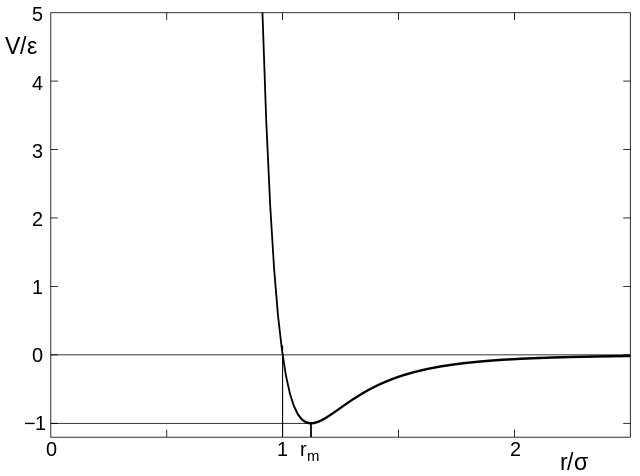
\includegraphics[width=9cm, keepaspectratio=true]{sections/cosserat_rods/images/LJpotential}
    \end{figure}
    
    the \textbf{Lennard-Jones potential} models the interaction between two atoms or molecules that are neutral and have no chemical bonds between them
    
    \vspace{0.3em}
    $\leftarrow$ potential energy as a function of the distance between the two atoms or molecules
    
    \vspace{-1em}
    \begin{displaymath}
      V(r) = 4 \cdot \epsilon \cdot \Biggl( \biggl( \frac{\sigma}{r} \biggr)^{12} - \biggl( \frac{\sigma}{r} \biggr)^6 \Biggr)
    \end{displaymath}
    
  \end{multicols}
\end{frame}


%-------------------------------------------------------------------------------
\begin{frame}
  \frametitle{Minimizing the energy of the unit cell (part 2)}

  \textbf{unit cell energy}
  \begin{displaymath}
    E = \frac{1}{2} \sum_{\alpha} \sum_{\beta} V(r_{\alpha, \beta})
  \end{displaymath}
  \begin{itemize}
    \item $\alpha$ iterates over the basis atoms of the unit cell
    \item $\beta$ iterates over all neighbors of $\alpha$ (also within the neighboring unit cells)
    \item a cutoff-radius defines the size of this neighborhood
    \item the factor $1/2$ comes from the fact that every bond appears twice: $(\alpha, \beta) \leftrightarrow (\beta, \alpha)$
    \item bonds that cross the boundary of the unit cell have a part inside and a part outside of the unit cell ; this symmetry implies that for every such bond only the part inside the unit cell is taken into account because the inside part of $(\alpha, \beta)$ equals exactly the outside part of $(\beta, \alpha)$ ; this works out regardless of the energy potential model $V$, i.e. also for models that are not pair-potentials 
  \end{itemize}
  % TODO work on more precise formulation

\end{frame}


%-------------------------------------------------------------------------------
\begin{frame}
  \frametitle{Direct molecular approach (part 1)}
  
  \begin{itemize}
    \item for larger deformations of a rod / nanotube the translational periodicity of the crystalline material is not preserved \newline
      $\rightarrow$ standard Cauchy Born rule cannot be used to compute the energy of a unit cell
    \item the idea is to \textit{directly} obtain $\psi \bigl( \underline{v}, \, \underline{k} \bigr)$, i.e. without first computing $W \bigl( \doubleunderline{F} \bigr)$
    \item the direct molecular approach takes care of surface effects
    \item and it can still be used whenever the rod cannot be thought of as a 3D continuum, \newline because e.g. the rod consists only of a wall with a thickness of one atom (SWCNT)
  \end{itemize}
  
  \vspace{0.5em}
  schematic of a SWCNT:
  
  \vspace{-2em}
  \begin{figure}
      \centering
      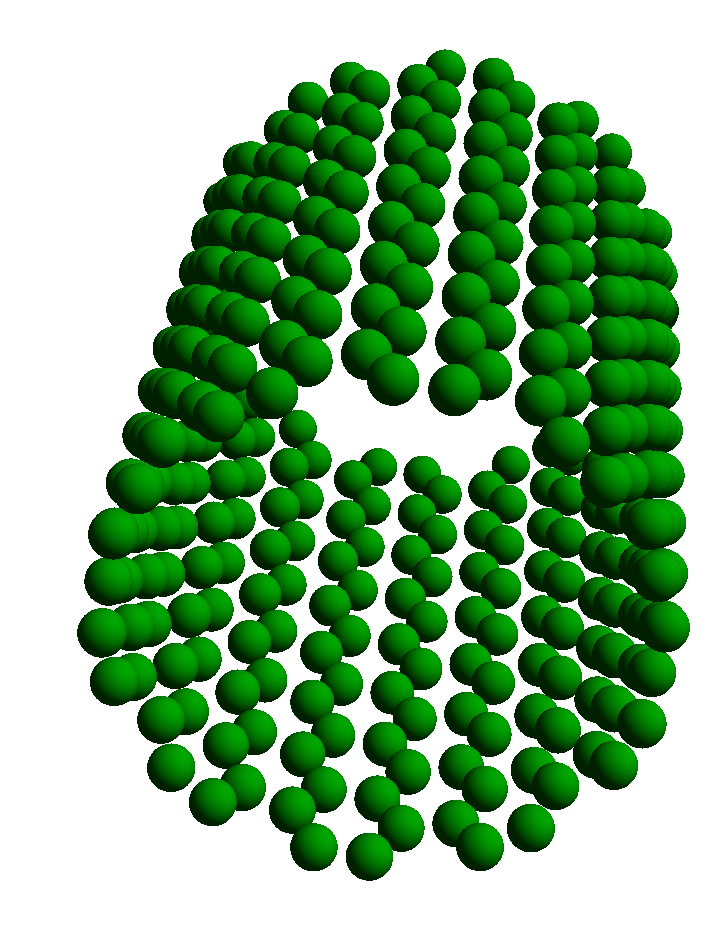
\includegraphics[width=6cm, keepaspectratio=true]{sections/cosserat_rods/images/SWCNT}
  \end{figure}
  % TODO star-problem
  
\end{frame}


%-------------------------------------------------------------------------------
\begin{frame}
  \frametitle{Direct molecular approach (part 2)}
  \vspace{-0.4em}
  \begin{multicols}{2}
    \begin{figure}
      \centering
      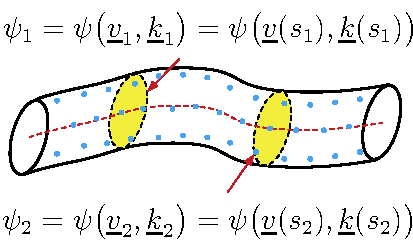
\includegraphics[width=10cm, keepaspectratio=true]{sections/cosserat_rods/images/LocalEnergyNano}
    \end{figure}
    %$\rightarrow$ for a nanorod we could count the individual atoms
    
    \vspace{1em}
    $\rightarrow$ we will again subject the rod to constant $\bigl( \underline{v} , \, \underline{k} \bigr)\, \forall s$ to obtain $\psi \bigl( \underline{v} , \, \underline{k} \bigr)$
    
    \vspace{0.5em}  
    \begin{figure}
      \centering
      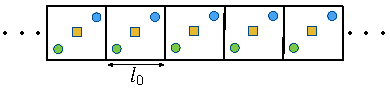
\includegraphics[width=11cm, keepaspectratio=true]{sections/cosserat_rods/images/1D-Crystal2}
    \end{figure}
    $\rightarrow$ the nanorod can be thought of as a 1D crystal, i.e. it has a unit cell that repeats only along $\underline{e}_3$-axis ; this repeating unit is sometimes also called fundamental domain
    
    \vspace{1em}
    $\rightarrow$ all unit cells deform in the same way for constant $\bigl( \underline{v} , \, \underline{k} \bigr) \forall s$
  \end{multicols}
  
\end{frame}


%-------------------------------------------------------------------------------
\begin{frame}
  \frametitle{Direct molecular approach (part 3)}

  \textbf{deformation map} for the repeating unit cells
  
  \vspace{0.2em}
  the reference state is given by $\underline{X}_{i,j}$
  \begin{itemize} 
    \item $i$ is an integer that indicates a particular unit cell (analog to the continuous scalar $s$)
    \item $j$ is an integer that indicates a particular basis atom within the unit cell \newline (analog to the continuous scalars $X_1$, $X_2$)
  \end{itemize}
  
  \vspace{0.5em}
  we want to determine $\underline{x}_{i,j}$ for a nanorod subjected to constant $\bigl( \underline{v} , \, \underline{k} \bigr) \forall s$
  
  \vspace{0.2em}
  the idea is to find a discrete analog of the 3D deformation map
  \begin{displaymath}
    \underline{x}(X_1, X_2, s) = 
    \underbrace{ \underline{x}_f + \exp \bigl( s \cdot \doubleunderline{K} \bigr) \cdot \biggl( \underline{x}_0(X_1,X_2) - \underline{x}_f \biggr) }_{\text{rotate cross section } s=0 } + 
    \underbrace{ s \cdot \tau \cdot \underline{\hat{k}} }_{\text{translate cross section}}
  \end{displaymath}
  
  \vspace{0.5em}
  with $s \rightarrow i \cdot l_0$ we get
  \begin{displaymath}
    \underline{x}_{i,j} = 
    \underbrace{ \underline{x}_f + \exp \bigl( i \cdot l_0 \cdot \doubleunderline{K} \bigr) \cdot \biggl( \underline{x}_{0,j} - \underline{x}_f \biggr) }_{\text{rotate unit cell } i=0 } + 
    \underbrace{ i \cdot l_0 \cdot \tau \cdot \underline{\hat{k}} }_{\text{translate unit cell}}
  \end{displaymath}
  
  \vspace{0.2em}
  $\rightarrow$ the atomic positions $\underline{x}_{0,j}$ in the unit cell $i=0$ are the unknowns we have to solve for  
\end{frame}


%-------------------------------------------------------------------------------
\begin{frame}
  \frametitle{Direct molecular approach (part 4)}

  \textbf{short recap}
  \begin{figure}
    \centering
    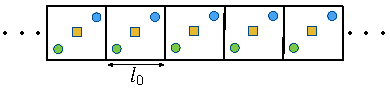
\includegraphics[width=17cm, keepaspectratio=true]{sections/cosserat_rods/images/1D-Crystal2}
  \end{figure}
  \begin{itemize}
    \item unit cells are the analogs of cross sections: $s \rightarrow i \cdot l_0$ with $i = 0, \, \dots,$
    \item the atomic positions in the unit cell $i=0$ are given by $\bigl( \underline{x}_{0,j} \bigr)_{j=0,\dots,M}$ \newline with the number of basis atoms $M=3$ in the example picture above
    \item for constant $\bigl( \underline{v} , \, \underline{k} \bigr) \forall s$ we get the discrete deformation map
        \begin{displaymath}
          \underline{x}_{i,j} = 
          \underline{x}_f + \exp \bigl( i \cdot l_0 \cdot \doubleunderline{K} \bigr) \cdot \biggl( \underline{x}_{0,j} - \underline{x}_f \biggr) + 
          i \cdot l_0 \cdot \tau \cdot \underline{\hat{k}}
        \end{displaymath}
    \item $\bigl( \underline{x}_{0,j} \bigr)_{j=1,\dots,M}$ are not functions as in the continuous case (no dependence on $X_1,X_2$)
  \end{itemize}
\end{frame}


%-------------------------------------------------------------------------------
\begin{frame}
  \frametitle{Direct molecular approach (part 5)}

  %TODO question: is the discrete crystal really following this map, that comes from continuum theory?
  
  \begin{itemize}
    \item reference state of the unit cell at $i=0$ given by $\bigl( \underline{X}_{0,j} \bigr)_{j=1,\dots,M}$
    \item reference state of entire crystal given by $\underline{X}_{0,j} = i \cdot l_0 \cdot \underline{e}_3 + \underline{X}_{0,j}$
    \item we apply a deformation such that the strains $\underline{v},\,\underline{k}$ are constant for all $s$
    \item we obtain the unknown $\underline{x}_{0,j}$ by minimizing the unit cell energy:
      \begin{displaymath}
        \underline{x}_{0,j} = \argmin_{(\underline{x}_{0,j})} E \bigl( \underline{x}_{0,1}, \, \dots , \, \underline{x}_{0,M} \, ; \, \underline{v}, \, \underline{k} \bigr) 
      \end{displaymath}
    \item the minimization is carried out subject to constraints: \newline
      (mass) center and orientation of the unit cell must be preserved, i.e.
      \begin{displaymath}
        %\int \rho_0 \cdot \underline{x}_0 \dif X_1 \dif X_2 =
        %\int \underline{x}_0 \dif m = \underline{0}
        %\: \rightarrow \:
        \sum_{j=1}^M m_j \cdot \underline{x}_{0,j} = \underline{0}
      \end{displaymath}
      and
      \begin{displaymath}
        %\int \underline{M} \dif X_1 \dif X_2 = \underline{0}
        %\: \rightarrow \:
        \sum_{j=1}^M 
        \underbrace{ m_j \cdot 
        \begin{bmatrix}
          x_2 \cdot x_3 \\
          x_1 \cdot x_3 \\
          x_1 \cdot x_2 
        \end{bmatrix} }_{=: \underline{M}_j} = \underline{0}
      \end{displaymath}
      
      \vspace{-1.2em}
      with $x_1,x_2,x_3$ the components of $\underline{x}_{0,j}$
  \end{itemize}
\end{frame}


%-------------------------------------------------------------------------------
\begin{frame}
  \frametitle{Direct molecular approach (part 6)}

  \textbf{minimization of energy under constraints}
  \begin{displaymath}
    \min_{(\underline{x}_{0,j} \, ; \, \underline{\lambda} , \, \underline{\mu} )} E \bigl( \underline{x}_{0,1}, \, \dots , \, \underline{x}_{0,M} \, ; \, \underline{v}, \, \underline{k} \bigr) +
    \underline{\lambda} \cdot \sum_{j=1}^M m_j \cdot \underline{x}_{0,j} +
    \underline{\mu} \cdot \sum_{j=1}^M \underline{M}_j
  \end{displaymath}
  
  \vspace{0.5em}
  setting the \textbf{first derivative} to zero we obtain
  \begin{displaymath}
    \pd{E}{\underline{x}_{0,j}} + 
    m_j \cdot \underline{\lambda} + 
    \underbrace{ m_j \cdot
    \begin{bmatrix}
      0 & x_3 & x_2 \\
      x_3 & 0 & x_1 \\
      x_2 & x_1 & 0
    \end{bmatrix} }_{=: \doubleunderline{M}_j} \cdot \underline{\mu} =
    \underline{0}
    \quad \forall j=1,\dots,M
  \end{displaymath}
  
  together with the 2 constraint equations this gives a system of $3 \, M + 6$ algebraic equations
  
  
\end{frame}


%-------------------------------------------------------------------------------
\begin{frame}
  \frametitle{Direct molecular approach (part 7)}
  \begin{displaymath}
    -\pd{E}{\underline{x}_{0,j}} = 
    m_j \cdot \underline{\lambda} + 
    \doubleunderline{M}_j \cdot \underline{\mu}
    \quad \forall j=1,\dots,M
  \end{displaymath}
  
  \vspace{0.5em}
  physical meaning:
  \begin{itemize}
    \item $-\pd{E}{\underline{x}_{0,j}}$ is the force on basis atom $j$ (due to its bond interactions with all other atoms)
    \item $\bigl( m_j \cdot \underline{\lambda} + \doubleunderline{M}_j \cdot \underline{\mu} \bigr)$ is the external force on basis atom $j$ that is required to keep the nanorod in the uniform configuration $\bigl( \underline{v},\underline{k} \bigr)$
  \end{itemize}
  
  \vspace{0.6em}
  in the case of pure bending or combined extension \& torsion the extra constraint forces $\bigl( m_j \cdot \underline{\lambda} + \doubleunderline{M}_j \cdot \underline{\mu} \bigr)$ are zero, i.e. no such forces are required to hold the beam in that configuration

\end{frame}


%-------------------------------------------------------------------------------
\begin{frame}
  \frametitle{Direct molecular approach (part 8)}

  the \textbf{strain energy density of the nanorod} is then given by
  \begin{displaymath}
    \psi \bigl( \underline{v}, \, \underline{k} \bigr) =
    \frac{1}{l_0} \cdot E \bigl( \underline{\hat{x}}_{0,1}(\underline{v},\underline{k}), \, \dots, \, \underline{\hat{x}}_{0,M}(\underline{v},\underline{k}) \, ; \, \underline{v}, \, \underline{k} \bigr)
  \end{displaymath}
  with
  \begin{displaymath}
    \bigl( \underline{\hat{x}}_{0,j}(\underline{v},\underline{k}) \bigr)_{j=1,\dots,M}= \argmin_{(\underline{x}_{0,j})_{j=1,\dots,M}} E \bigl( \underline{x}_{0,1}, \, \dots , \, \underline{x}_{0,M} \, ; \, \underline{v}, \, \underline{k} \bigr)
  \end{displaymath}
  such that the kinematic constraints are satisfied
  
  \vspace{1em}
  for further information on this topic please consider reading the paper ``A Helical Cauchy-Born Rule for Special Cosserat Rod Modeling of Nano and Continuum Rods'' by Kumar et al. in Journal of Elasticity 124, June 2016
  
\end{frame}

%TODO twist example from lecture, further information?
% same environment up to a finite rotation


%===============================================================================
\subsection{FEM discretization}

%-------------------------------------------------------------------------------
\begin{frame}
  \frametitle{Weak form of the equations (part 1)}

  by multiplying the \textbf{strong form} of the equations
  \begin{displaymath}
    \underline{n}^{\prime}(s) + \underline{\hat{n}}(s) =
    \rho_0 \cdot A \cdot \underline{\ddot{r}}(s)
  \end{displaymath}
  \begin{displaymath}
    \underline{m}^{\prime}(s) + \underline{r}^{\prime}(s) \times \underline{n}(s) + \underline{\hat{m}}(s) =
    \rho_0 \cdot
    \od{}{t} \bigl( \doubleunderline{I}_0 \cdot \underline{\omega} \bigr)
  \end{displaymath}
  with test functions $\delta \underline{r}(s)$ and $\delta \underline{\Theta}(s)$ respectivly and integrating over the length of the rod we get a weak form of the equations ...
  \begin{displaymath}
    \int_0^L \biggl( \underline{n}^{\prime}(s) + \underline{\hat{n}}(s) \biggr) \cdot \delta \underline{r}(s) \: \dif s  =
    \int_0^L \rho_0 \cdot A \cdot \underline{\ddot{r}}(s) \cdot \delta \underline{r}(s) \: \dif s
  \end{displaymath}
  \begin{displaymath}
    \int_0^L \biggl( \underline{m}^{\prime}(s) + \underline{r}^{\prime}(s) \times \underline{n}(s) + \underline{\hat{m}}(s) \biggr) \cdot \delta \underline{\Theta}(s) \: \dif s =
    \int_0^L \rho_0 \cdot
    \od{}{t} \bigl( \doubleunderline{I}_0 \cdot \underline{\omega} \bigr) \cdot \delta \underline{\Theta}(s) \: \dif s
  \end{displaymath}
  
  where $\doubleunderline{I}_0$ is the moment of area tensor
 
\end{frame}


%-------------------------------------------------------------------------------
\begin{frame}
  \frametitle{Weak form of the equations (part 2)}
   
  by adding both equations together we obtain the \textbf{weak form}
  \begin{displaymath}
    G = 
    \underbrace{
    \int_0^L \biggl(
    \rho_0 \cdot A \cdot \underline{\ddot{r}}(s) \cdot \delta \underline{r}(s) +
    \rho_0 \cdot \od{}{t} \bigl( \doubleunderline{I}_0 \cdot \underline{\omega} \bigr) \cdot \delta \underline{\Theta}(s)
    \biggr) \: \dif s
    }_{=: G_{\text{dyn}}}
  \end{displaymath}
  \begin{displaymath}
    \underbrace{
    - \int_0^L \biggl( \underline{n}^{\prime}(s) + \underline{\hat{n}}(s) \biggr) \cdot \delta \underline{r}(s) \: \dif s
    - \int_0^L \biggl( \underline{m}^{\prime}(s) + \underline{r}^{\prime}(s) \times \underline{n}(s) + \underline{\hat{m}}(s) \biggr) \cdot \delta \underline{\Theta}(s) \: \dif s
    }_{=: G_{\text{stat}}}
  \end{displaymath}
  
  \vspace{1em}
  since the internal contact force $\underline{n}(s)$ and the internal moment $\underline{m}(s)$ depend on the strains $\underline{v}(s)$ and $\underline{k}(s)$ they are of first order in the kinematic variables $\underline{r}(s)$ and $\underline{\Theta}(s)$ \newline
  with $\doubleunderline{R}(s) = \exp \bigl( \doubleunderline{\Theta}(s) \bigr) = \exp \bigl( [\underline{\Theta}]_{\times} \bigr)$
  
  \vspace{0.5em}
  $\rightarrow$ $\underline{n}^{\prime}(s)$ and $\underline{m}^{\prime}(s)$ are therefore of second order in the kinematic variables

\end{frame}


%-------------------------------------------------------------------------------
\begin{frame}
  \frametitle{Weak form of the equations (part 3)}
  
  we can relax the regularity requirements for a solution by transferring one order of the derivatives onto the test functions via integration by parts ...
  \begin{displaymath}
    G_{\text{stat}} =
    - \int_0^L \biggl( 
        \bigl( \underline{n}(s) \cdot \delta \underline{r}(s) \bigr)^{\prime}
      - \underline{n}(s) \cdot \delta \underline{r}^{\prime}(s)
      + \bigl( \underline{m}(s) \cdot \delta \underline{\Theta}(s) \bigr)^{\prime}
      - \underline{m}(s) \cdot \delta \underline{\Theta}^{\prime}(s) \: +
  \end{displaymath}
  \begin{displaymath}
      + \: \underline{\hat{n}}(s) \cdot \delta \underline{r}(s)
      + \underline{\hat{m}}(s) \cdot \delta \underline{\Theta}(s)
      + \bigl( \underline{r}^{\prime}(s) \times \underline{n}(s) \bigr) \cdot \delta \underline{\Theta}(s)    
    \biggr) \: \dif s =
  \end{displaymath}
  \begin{displaymath}
    = 
    \overbrace{
      \int_0^L \biggl( 
        \underline{n}(s) \cdot \delta \underline{r}^{\prime}(s)
      + \underline{m}(s) \cdot \delta \underline{\Theta}^{\prime}(s)
      + \bigl( \underline{n}(s) \times \underline{r}^{\prime}(s) \bigr) \cdot \delta \underline{\Theta}(s)
      \biggr) \: \dif s \: 
    }^{\text{internal response}} + 
  \end{displaymath}
  \begin{displaymath}
    \overbrace{
    - \int_0^L \biggl( 
        \underline{\hat{n}}(s) \cdot \delta \underline{r}(s)
      + \underline{\hat{m}}(s) \cdot \delta \underline{\Theta}(s)
     \biggr) \: \dif s \:
    }^{\text{external distributed loads}}
    \overbrace{
    - \biggl(
      \underline{n}_p(s) \cdot \delta \underline{r}(s) +
      \underline{m}_p(s) \cdot \delta \underline{\Theta}(s)
    \biggr) \sVert[2]_0^L
    }^{\text{external loads at boundaries}}
  \end{displaymath}
  
  \vspace{0.5em}
  with $\underline{n}_p$ and $\underline{m}_p$ as prescribed quantities at the boundary \newline
  whereas $\underline{n}(s)$ and $\underline{m}(s)$ are obtained from constitutive law
\end{frame}


%-------------------------------------------------------------------------------
\begin{frame}
  \frametitle{Weak form of the equations (part 4)}
  
  changing the order of the scalar triple product gives ...
  \begin{displaymath}
    G_{\text{stat}} = 
    \overbrace{
      \int_0^L \biggl( 
        \underline{n}(s) \cdot \delta \underline{r}^{\prime}(s)
      + \underline{m}(s) \cdot \delta \underline{\Theta}^{\prime}(s)
      + \underline{n}(s) \cdot \bigl( \underline{r}^{\prime}(s) \times \delta \underline{\Theta}(s) \bigr)
      \biggr) \: \dif s \: 
    }^{\text{internal response}} + 
  \end{displaymath}
  \begin{displaymath}
    \overbrace{
    - \int_0^L \biggl( 
        \underline{\hat{n}}(s) \cdot \delta \underline{r}(s)
      + \underline{\hat{m}}(s) \cdot \delta \underline{\Theta}(s)
     \biggr) \: \dif s
    }^{\text{external distributed loads}} \:
    \overbrace{
    - \biggl(
      \underline{n}_p(s) \cdot \delta \underline{r}(s) +
      \underline{m}_p(s) \cdot \delta \underline{\Theta}(s)
    \biggr) \sVert[2]_0^L
    }^{\text{external loads at boundaries}}
  \end{displaymath}
  
  \vspace{1em}
  we can write the internal part in a more compact form by introducing the operator
  \begin{displaymath}
    \doubleunderline{E}^{\mathrm{T}}(s) =
    \begin{bmatrix}
      \doubleunderline{I} \, \od{}{s} & [ \underline{r}^{\prime}(s) ]_{\times} \\
      \doubleunderline{0}             & \doubleunderline{I} \, \od{}{s}
    \end{bmatrix}
  \end{displaymath}
  \begin{displaymath}
    G_{\text{stat}} = 
    \overbrace{
      \int_0^L
        \begin{bmatrix}
          \underline{n} \\ \underline{m}
        \end{bmatrix}
        \cdot \doubleunderline{E}^{\mathrm{T}}(s) \cdot
        \begin{bmatrix}
          \delta \underline{r} \\ \delta \underline{\Theta}
        \end{bmatrix}
      \: \dif s 
    }^{\text{internal response}} \:
    \overbrace{
      - \int_0^L
        \begin{bmatrix}
          \underline{\hat{n}} \\ \underline{\hat{m}}
        \end{bmatrix} \cdot
        \begin{bmatrix}
          \delta \underline{r} \\ \delta \underline{\Theta}
        \end{bmatrix}
      \: \dif s
    }^{\text{external distributed loads}} \:
    \overbrace{
      - \begin{bmatrix}
          \underline{n}_p \\ \underline{m}_p
      \end{bmatrix} \cdot
      \begin{bmatrix}
          \delta \underline{r} \\ \delta \underline{\Theta}
      \end{bmatrix}
      \sVert[3]_0^L
    }^{\text{external loads at boundaries}}
  \end{displaymath}

\end{frame}



%-------------------------------------------------------------------------------
\begin{frame}
  \frametitle{Weak form of the equations (part 5)}
  
  the weak form of the problem is
  \begin{displaymath}
    G = G_{\text{dyn}} + G_{\text{stat}} = 0
    \quad \forall \bigl( \delta \underline{r} , \, \delta \underline{\Theta} \bigr) \: \text{admissible}
  \end{displaymath}
  admissible means that the test functions must satisfy the kinematic boundary conditions
  
  \vspace{1em}
  in the sequel we will work with the \textbf{static problem}, i.e. we assume $G_{\text{dyn}} \equiv 0$
  
  \vspace{0.5em}
  the weak form $G_{\text{stat}} \bigl( \underline{r} , \, \underline{\Theta} \, ; \, \delta \underline{r} , \, \delta \underline{\Theta} \bigr)$ is 
  \begin{itemize}
    \item nonlinear in the unknowns $\bigl( \underline{r} , \, \underline{\Theta} \bigr)$
    \item and linear in the test functions $\bigl( \delta \underline{r} , \, \delta \underline{\Theta} \bigr)$
  \end{itemize}
  
  \vspace{0.5em}
  in order to find a solution we must linearize the weak form and solve iteratively ...

\end{frame}


%-------------------------------------------------------------------------------
\begin{frame}
  \frametitle{Linearization of the weak form (part 1)}
  
  we introduce \textbf{perturbed versions of the unknowns}
  \begin{displaymath}
    \underline{r}_{\epsilon}(s) = \underline{r}(s) + \epsilon \cdot \Delta \underline{r}(s)
    \quad \text{and} \quad
    \doubleunderline{R}_{\epsilon}(s) = \exp \bigl( \epsilon \cdot \Delta \doubleunderline{\Theta}(s) \bigr) \cdot \exp \bigl( \doubleunderline{\Theta}(s) \bigr)
  \end{displaymath}
  with $\Delta \underline{r}$ the increment in $\underline{r}$ and $\Delta \underline{\Theta} = \axial \bigl( \Delta \doubleunderline{\Theta} \bigr)$ the increment in $\underline{\Theta}$
  
  \vspace{1em}
  we then obtain the \textbf{linearized weak form} by truncating the Taylor expansion of $G_{\text{stat}} \bigl( \underline{r}_{\epsilon} , \, \underline{\Theta}_{\epsilon} \, ; \, \delta \underline{r} , \, \delta \underline{\Theta} \bigr)$ in $\epsilon$ after the linear term
  \begin{displaymath}
    \underbrace{
    G_{\text{stat}} \bigl( \underline{r}_{\epsilon} , \, \underline{\Theta}_{\epsilon} \, ; \, \delta \underline{r} , \, \delta \underline{\Theta} \bigr)
    }_{\text{should equal 0}} \approx
    \underbrace{
    G_{\text{stat}} \bigl( \underline{r} , \, \underline{\Theta} \, ; \, \delta \underline{r} , \, \delta \underline{\Theta} \bigr) +
    \od{}{\epsilon} \, G_{\text{stat}} \bigl( \underline{r}_{\epsilon} , \, \underline{\Theta}_{\epsilon} \, ; \, \delta \underline{r} , \, \delta \underline{\Theta} \bigr) \sVert[2]_{\epsilon=0} \cdot \epsilon 
    }_{\text{linearized weak form}}
    + \xcancel{\text{HOT}}
  \end{displaymath}
  
\end{frame}


%-------------------------------------------------------------------------------
\begin{frame}
  \frametitle{Linearization of the weak form (part 2)}
  
  for simplicity we now assume $\underline{\hat{n}}(s) \equiv 0$, $\underline{\hat{m}}(s) \equiv 0$ and we also ignore the boundary terms \newline
  so we only have   
  \begin{displaymath}
    G_{\text{stat}} = 
    \int_0^L
      \begin{bmatrix}
        \underline{n}(s) \\ \underline{m}(s)
      \end{bmatrix}
      \cdot \doubleunderline{E}^{\mathrm{T}}(s) \cdot
      \begin{bmatrix}
        \delta \underline{r}(s) \\ \delta \underline{\Theta}(s)
      \end{bmatrix}
    \: \dif s \:
%    - \begin{bmatrix}
%        \underline{n}_p(s) \\ \underline{m}_p(s)
%    \end{bmatrix} \cdot
%    \begin{bmatrix}
%        \delta \underline{r}(s) \\ \delta \underline{\Theta}(s)
%    \end{bmatrix}
%    \sVert[4]_0^L
  \end{displaymath}

  \vspace{0.5em}
  we introduce the perturbed version of $G_{\text{stat}}$
  \begin{displaymath}
    G_{\text{stat}}^{\epsilon} = 
    \int_0^L
      \begin{bmatrix}
        \underline{n}_{\epsilon}(s) \\ \underline{m}_{\epsilon}(s)
      \end{bmatrix}
      \cdot \doubleunderline{E}_{\epsilon}^{\mathrm{T}}(s) \cdot
      \begin{bmatrix}
        \delta \underline{r}(s) \\ \delta \underline{\Theta}(s)
      \end{bmatrix}
    \: \dif s %\:
    %- \begin{bmatrix}
    %    \underline{n}_p(s) \\ \underline{m}_p(s)
    %\end{bmatrix} \cdot
    %\begin{bmatrix}
    %    \delta \underline{r}(s) \\ \delta \underline{\Theta}(s)
    %\end{bmatrix}
    %\sVert[4]_0^L
    % TODO + \dots
  \end{displaymath}
  
  \vspace{0.5em}
  and compute the first derivative at $\epsilon = 0$
  \begin{displaymath}
    \od{}{\epsilon} \, G_{\text{stat}}^{\epsilon} \sVert[3]_{\epsilon=0} =
    \int_0^L \od{}{\epsilon}
      \begin{bmatrix}
        \underline{n}_{\epsilon} \\ \underline{m}_{\epsilon}
      \end{bmatrix} \sVert[4]_{\epsilon=0} \cdot
      \doubleunderline{E}^{\mathrm{T}} \cdot
      \begin{bmatrix}
        \delta \underline{r} \\ \delta \underline{\Theta}
      \end{bmatrix}
    \: \dif s \: +
    \int_0^L 
      \begin{bmatrix}
        \underline{n} \\ \underline{m}
      \end{bmatrix} \cdot
      \od{}{\epsilon} \, \doubleunderline{E}_{\epsilon}^{\mathrm{T}} \sVert[3]_{\epsilon=0} \cdot
      \begin{bmatrix}
        \delta \underline{r} \\ \delta \underline{\Theta}
      \end{bmatrix}
    \: \dif s
  \end{displaymath}
  
  \vspace{1em}
  in the sequel we will compute the individual terms of the first derivative step by step and then recompile the results

\end{frame}


%-------------------------------------------------------------------------------
\begin{frame}
  \frametitle{Linearization of the weak form (part 3)}

  the linearization of the internal contact force is
  \begin{displaymath}
    \od{}{\epsilon} \, \underline{n}_{\epsilon} \sVert[3]_{\epsilon=0} = 
    \od{}{\epsilon} \biggl(
      \doubleunderline{R}_{\epsilon} \cdot \pd{\psi}{\underline{v}} \bigl( \underline{v}_{\epsilon}, \, \underline{k}_{\epsilon} \bigr)
    \biggr) \sVert[3]_{\epsilon=0} =
    \od{}{\epsilon} \, \doubleunderline{R}_{\epsilon} \sVert[3]_{\epsilon=0} \cdot \pd{\psi}{\underline{v}} \bigl( \underline{v}, \, \underline{k} \bigr) +
    \doubleunderline{R} \cdot \od{}{\epsilon} \biggl( \pd{\psi}{\underline{v}} \bigl( \underline{v}_{\epsilon}, \, \underline{k}_{\epsilon} \bigr) \biggr) \sVert[3]_{\epsilon=0}
  \end{displaymath}
  
  \vspace{1em}
  with
  \begin{displaymath}
    \od{}{\epsilon} \, \doubleunderline{R}_{\epsilon} \sVert[3]_{\epsilon=0} =
    \od{}{\epsilon} \biggl( \exp \bigl( \epsilon \cdot \Delta \doubleunderline{\Theta} \bigr) \cdot \doubleunderline{R} \biggr) \sVert[3]_{\epsilon=0} =
    \od{}{\epsilon} \exp \bigl( \epsilon \cdot \Delta \doubleunderline{\Theta} \bigr) \sVert[3]_{\epsilon=0} \cdot \doubleunderline{R} =
    \Delta \doubleunderline{\Theta} \cdot \doubleunderline{R}
  \end{displaymath}
  
  \vspace{1em}
  and
  \begin{displaymath}
    \od{}{\epsilon} \biggl( \pd{\psi}{\underline{v}} \bigl( \underline{v}_{\epsilon}, \, \underline{k}_{\epsilon} \bigr) \biggr) \sVert[3]_{\epsilon=0} =
    \pd[2]{\psi}{\underline{v}} \cdot \od{\underline{v}_{\epsilon}}{\epsilon} \sVert[3]_{\epsilon=0}
     + \md{\psi}{2}{\underline{v}}{}{\underline{k}}{} \cdot \od{\underline{k}_{\epsilon}}{\epsilon} \sVert[3]_{\epsilon=0}
  \end{displaymath}
  
  \vspace{0.5em}
  and the linearized strains (cf. pages \autoref{eq:fist_variation_of_v} and \autoref{eq:fist_variation_of_k})
  \begin{displaymath}
    \od{\underline{v}_{\epsilon}}{\epsilon} \sVert[3]_{\epsilon=0} =
    \od{}{\epsilon} \, \bigl( \doubleunderline{R}_{\epsilon}^{\mathrm{T}} \cdot \underline{r}_{\epsilon}^{\prime} \bigr) \sVert[3]_{\epsilon=0} =
    \doubleunderline{R}^{\mathrm{T}} \cdot \bigl( \Delta \underline{r}^{\prime} + \underline{r}^{\prime} \times \Delta \underline{\Theta} \bigr)
    \quad \text{and} \quad
    \od{\underline{k}_{\epsilon}}{\epsilon} \sVert[3]_{\epsilon=0} =
    \doubleunderline{R}^{\mathrm{T}} \cdot \Delta \underline{\Theta}^{\prime}
  \end{displaymath}
  
\end{frame}


%-------------------------------------------------------------------------------
\begin{frame}
  \frametitle{Linearization of the weak form (part 4)}
  
  plugging back in gives ...
  \begin{displaymath}
    \od{}{\epsilon} \, \underline{n}_{\epsilon} \sVert[3]_{\epsilon=0} = 
    \Delta \doubleunderline{\Theta} \cdot \doubleunderline{R} \cdot \pd{\psi}{\underline{v}} +
    \doubleunderline{R} \cdot
    \begin{bmatrix}
      \pd[2]{\psi}{\underline{v}} & \md{\psi}{2}{\underline{v}}{}{\underline{k}}{}
    \end{bmatrix} \cdot
    \begin{bmatrix}
      \doubleunderline{R}^{\mathrm{T}} \cdot \bigl( \Delta \underline{r}^{\prime} + \underline{r}^{\prime} \times \Delta \underline{\Theta} \bigr) \\
      \doubleunderline{R}^{\mathrm{T}} \cdot \Delta \underline{\Theta}^{\prime} =
    \end{bmatrix}
  \end{displaymath}
  \begin{displaymath}
    = - \underline{n} \times \Delta \underline{\Theta} + 
    \doubleunderline{R} \cdot
    \begin{bmatrix}
      \pd[2]{\psi}{\underline{v}} & \md{\psi}{2}{\underline{v}}{}{\underline{k}}{}
    \end{bmatrix} \cdot
    \begin{bmatrix}
      \doubleunderline{R}^{\mathrm{T}} \cdot \bigl( \Delta \underline{r}^{\prime} + \underline{r}^{\prime} \times \Delta \underline{\Theta} \bigr) \\
      \doubleunderline{R}^{\mathrm{T}} \cdot \Delta \underline{\Theta}^{\prime} =
    \end{bmatrix}
  \end{displaymath}
  
  
  \vspace{1em}
  likewise the linearization of the internal moment is
  \begin{displaymath}
    \od{}{\epsilon} \, \underline{m}_{\epsilon} \sVert[3]_{\epsilon=0} = 
    \od{}{\epsilon} \biggl(
      \doubleunderline{R}_{\epsilon} \cdot \pd{\psi}{\underline{k}} \bigl( \underline{v}_{\epsilon}, \, \underline{k}_{\epsilon} \bigr)
    \biggr) \sVert[3]_{\epsilon=0} =
    \od{}{\epsilon} \, \doubleunderline{R}_{\epsilon} \sVert[3]_{\epsilon=0} \cdot \pd{\psi}{\underline{k}} \bigl( \underline{v}, \, \underline{k} \bigr) +
    \doubleunderline{R} \cdot \od{}{\epsilon} \biggl( \pd{\psi}{\underline{k}} \bigl( \underline{v}_{\epsilon}, \, \underline{k}_{\epsilon} \bigr) \biggr) \sVert[3]_{\epsilon=0}
  \end{displaymath}
  
  \vspace{1em}
  with the first term already computed above and with
  \begin{displaymath}
    \od{}{\epsilon} \biggl( \pd{\psi}{\underline{k}} \bigl( \underline{v}_{\epsilon}, \, \underline{k}_{\epsilon} \bigr) \biggr) \sVert[3]_{\epsilon=0} =
     \md{\psi}{2}{\underline{k}}{}{\underline{v}}{} \cdot \od{\underline{v}_{\epsilon}}{\epsilon} \sVert[3]_{\epsilon=0} +
     \pd[2]{\psi}{\underline{k}} \cdot \od{\underline{k}_{\epsilon}}{\epsilon} \sVert[3]_{\epsilon=0}
  \end{displaymath}

  
\end{frame}


%-------------------------------------------------------------------------------
\begin{frame}
  \frametitle{Linearization of the weak form (part 5)}
  
  plugging back in gives ...
  \begin{displaymath}
    \od{}{\epsilon} \, \underline{m}_{\epsilon} \sVert[3]_{\epsilon=0} = 
    \Delta \doubleunderline{\Theta} \cdot \doubleunderline{R} \cdot \pd{\psi}{\underline{k}} +
    \doubleunderline{R} \cdot
    \begin{bmatrix}
      \md{\psi}{2}{\underline{k}}{}{\underline{v}}{} & \pd[2]{\psi}{\underline{k}}
    \end{bmatrix} \cdot
    \begin{bmatrix}
      \doubleunderline{R}^{\mathrm{T}} \cdot \bigl( \Delta \underline{r}^{\prime} + \underline{r}^{\prime} \times \Delta \underline{\Theta} \bigr) \\
      \doubleunderline{R}^{\mathrm{T}} \cdot \Delta \underline{\Theta}^{\prime} =
    \end{bmatrix} =
  \end{displaymath}
  \begin{displaymath}
    = - \underline{m} \times \Delta \underline{\Theta} +
    \doubleunderline{R} \cdot
    \begin{bmatrix}
      \md{\psi}{2}{\underline{k}}{}{\underline{v}}{} & \pd[2]{\psi}{\underline{k}}
    \end{bmatrix} \cdot
    \begin{bmatrix}
      \doubleunderline{R}^{\mathrm{T}} \cdot \bigl( \Delta \underline{r}^{\prime} + \underline{r}^{\prime} \times \Delta \underline{\Theta} \bigr) \\
      \doubleunderline{R}^{\mathrm{T}} \cdot \Delta \underline{\Theta}^{\prime} =
    \end{bmatrix} 
  \end{displaymath}
  
  \vspace{1em}
  we also linearize the introduced operator matrix ...
  \begin{displaymath}
    \doubleunderline{E}_{\epsilon}^{\mathrm{T}}(s) =
    \begin{bmatrix}
      \doubleunderline{I} \, \od{}{s} & [ \underline{r}_{\epsilon}^{\prime}(s) ]_{\times} \\
      \doubleunderline{0}             & \doubleunderline{I} \, \od{}{s}
    \end{bmatrix}
  \quad \Rightarrow \quad
    \od{}{\epsilon} \, \doubleunderline{E}_{\epsilon}^{\mathrm{T}} \sVert[3]_{\epsilon=0} =
    \begin{bmatrix}
      \doubleunderline{0} & [ \Delta \underline{r}^{\prime}(s) ]_{\times} \\
      \doubleunderline{0} & \doubleunderline{0}
    \end{bmatrix}
  \end{displaymath}
  
\end{frame}


%-------------------------------------------------------------------------------
\begin{frame}
  \frametitle{Linearization of the weak form (part 6)}

  finally we obtain the linearized weak form ...
  \begin{displaymath}
    \od{}{\epsilon} \, G_{\text{stat}}^{\epsilon} \sVert[3]_{\epsilon=0} =
    \int_0^L \Biggl(
      \begin{bmatrix}
        \doubleunderline{0} & - [ \underline{n} ]_{\times} \\
        \doubleunderline{0} & - [ \underline{m} ]_{\times}
      \end{bmatrix} \cdot
      \begin{bmatrix}
        \Delta \underline{r} \\
        \Delta \underline{\Theta}
      \end{bmatrix} +
    \end{displaymath}
    \begin{displaymath}
     + \underbrace{
      \begin{bmatrix}
        \doubleunderline{R} & \doubleunderline{0} \\
        \doubleunderline{0} & \doubleunderline{R}
      \end{bmatrix}}_{=: \doubleunderline{\pi}} \cdot
      \underbrace{
      \begin{bmatrix}
        \pd[2]{\psi}{\underline{v}} & \md{\psi}{2}{\underline{v}}{}{\underline{k}}{} \\
        \md{\psi}{2}{\underline{k}}{}{\underline{v}}{} & \pd[2]{\psi}{\underline{k}}
      \end{bmatrix}}_{=: \doubleunderline{H}} \cdot
      \begin{bmatrix}
        \doubleunderline{R}^{\mathrm{T}} & \doubleunderline{0} \\
        \doubleunderline{0} & \doubleunderline{R}^{\mathrm{T}}
      \end{bmatrix} \cdot
      \doubleunderline{E}^{\mathrm{T}} \cdot
      \begin{bmatrix}
        \Delta \underline{r} \\
        \Delta \underline{\Theta}
      \end{bmatrix} \Biggr) \cdot
      \doubleunderline{E}^{\mathrm{T}} \cdot
      \begin{bmatrix}
        \delta \underline{r} \\ \delta \underline{\Theta}
      \end{bmatrix}
    \: \dif s \: +
  \end{displaymath}
  \begin{displaymath}
   +\int_0^L
      \underbrace{
      \begin{bmatrix}
        \underline{n} \\ \underline{m}
      \end{bmatrix} \cdot
      \begin{bmatrix}
        \doubleunderline{0} & [ \Delta \underline{r}^{\prime} ]_{\times} \\
        \doubleunderline{0} & \doubleunderline{0}
      \end{bmatrix} \cdot
      \begin{bmatrix}
        \delta \underline{r} \\ \delta \underline{\Theta}
      \end{bmatrix}
      }_{
        \underline{n} \cdot \bigl( \Delta \underline{r}^{\prime} \times \delta \underline{\Theta} \bigr)
      }
    \: \dif s =
  \end{displaymath}
  \begin{displaymath}
    = \int_0^L
      \begin{bmatrix}
        \doubleunderline{0} & - [ \underline{n} ]_{\times} \\
        \doubleunderline{0} & - [ \underline{m} ]_{\times}
      \end{bmatrix} \cdot
      \begin{bmatrix}
        \Delta \underline{r} \\
        \Delta \underline{\Theta}
      \end{bmatrix} \cdot
      \doubleunderline{E}^{\mathrm{T}} \cdot
      \begin{bmatrix}
        \delta \underline{r} \\ \delta \underline{\Theta}
      \end{bmatrix}
    \: \dif s \:
    + \int_0^L
      \doubleunderline{\pi} \cdot
      \doubleunderline{H} \cdot
      \doubleunderline{\pi}^{\mathrm{T}} \cdot
      \doubleunderline{E}^{\mathrm{T}} \cdot
      \begin{bmatrix}
        \Delta \underline{r} \\
        \Delta \underline{\Theta}
      \end{bmatrix} \cdot
      \doubleunderline{E}^{\mathrm{T}} \cdot
      \begin{bmatrix}
        \delta \underline{r} \\ \delta \underline{\Theta}
      \end{bmatrix}
    \: \dif s \: +
  \end{displaymath}
  \begin{displaymath}
   + \int_0^L
      [ \underline{n} ]_{\times} \cdot \Delta \underline{r}^{\prime} \cdot \delta \underline{\Theta}
    \: \dif s
  \end{displaymath}

\end{frame}


%-------------------------------------------------------------------------------
\begin{frame}
  \frametitle{Linearization of the weak form (recap)}

  \vspace{-0.5em}
  \begin{displaymath}
    \overbrace{
    G_{\text{stat}} \bigl( \underline{r}_{\epsilon} , \, \underline{\Theta}_{\epsilon} \, ; \, \delta \underline{r} , \, \delta \underline{\Theta} \bigr) }^{\text{nonlinear weak form}} \equiv
    G_{\text{stat}} \bigl( \Delta \underline{r} , \, \Delta \underline{\Theta} \, ; \,\underline{r} , \, \underline{\Theta} \, ; \, \delta \underline{r} , \, \delta \underline{\Theta} \bigr) \approx
  \end{displaymath}
  \begin{displaymath}
    \approx
    \underbrace{
    G_{\text{stat}} \bigl( \underline{r} , \, \underline{\Theta} \, ; \, \delta \underline{r} , \, \delta \underline{\Theta} \bigr) +
    DG_{\text{stat}} \bigl( \Delta \underline{r} , \, \Delta \underline{\Theta} \, ; \,\underline{r} , \, \underline{\Theta} \, ; \, \delta \underline{r} , \, \delta \underline{\Theta} \bigr)
    }_{\text{linearized weak form}}
  \end{displaymath}
  
  \vspace{0.5em}
  with the nonlinear weak form
  \begin{displaymath}
    G_{\text{stat}} = 
      \int_0^L
        \begin{bmatrix}
          \underline{n} \\ \underline{m}
        \end{bmatrix}
        \cdot \doubleunderline{E}^{\mathrm{T}}(s) \cdot
        \begin{bmatrix}
          \delta \underline{r} \\ \delta \underline{\Theta}
        \end{bmatrix}
      \: \dif s \:
      - \int_0^L
        \begin{bmatrix}
          \underline{\hat{n}} \\ \underline{\hat{m}}
        \end{bmatrix} \cdot
        \begin{bmatrix}
          \delta \underline{r} \\ \delta \underline{\Theta}
        \end{bmatrix}
      \: \dif s \:
      - \begin{bmatrix}
          \underline{n}_p \\ \underline{m}_p
      \end{bmatrix} \cdot
      \begin{bmatrix}
          \delta \underline{r} \\ \delta \underline{\Theta}
      \end{bmatrix}
      \sVert[3]_0^L
  \end{displaymath}
  
  \vspace{0.7em}
  and the first order term from its Taylor expansion
  \begin{displaymath}
    DG_{\text{stat}} =
    \int_0^L
      \begin{bmatrix}
        \doubleunderline{0} & - [ \underline{n} ]_{\times} \\
        \doubleunderline{0} & - [ \underline{m} ]_{\times}
      \end{bmatrix} \cdot
      \begin{bmatrix}
        \Delta \underline{r} \\
        \Delta \underline{\Theta}
      \end{bmatrix} \cdot
      \doubleunderline{E}^{\mathrm{T}} \cdot
      \begin{bmatrix}
        \delta \underline{r} \\ \delta \underline{\Theta}
      \end{bmatrix}
    \: \dif s \:
    + \int_0^L
      \doubleunderline{\pi} \cdot
      \doubleunderline{H} \cdot
      \doubleunderline{\pi}^{\mathrm{T}} \cdot
      \doubleunderline{E}^{\mathrm{T}} \cdot
      \begin{bmatrix}
        \Delta \underline{r} \\
        \Delta \underline{\Theta}
      \end{bmatrix} \cdot
      \doubleunderline{E}^{\mathrm{T}} \cdot
      \begin{bmatrix}
        \delta \underline{r} \\ \delta \underline{\Theta}
      \end{bmatrix}
    \: \dif s \: +
  \end{displaymath}
  \begin{displaymath}
   + \int_0^L
      [ \underline{n} ]_{\times} \cdot \Delta \underline{r}^{\prime} \cdot \delta \underline{\Theta}
    \: \dif s
   + \dots (\text{first order terms of distributed load and boundary terms})
  \end{displaymath}
  
\end{frame}


%-------------------------------------------------------------------------------
\begin{frame}
  \frametitle{Iteratively solving the nonlinear problem}
  
  note that $DG_{\text{stat}} \bigl( \Delta \underline{r} , \, \Delta \underline{\Theta} \, ; \,\underline{r} , \, \underline{\Theta} \, ; \, \delta \underline{r} , \, \delta \underline{\Theta} \bigr)$ is
  \begin{itemize}
    \item linear in $\bigl( \Delta \underline{r} , \, \Delta \underline{\Theta} \bigr)$
    \item nonlinear in $\bigl( \underline{r} , \, \underline{\Theta} \bigr)$
    \item and linear in $\bigl( \delta \underline{r} , \, \delta \underline{\Theta} \bigr)$
  \end{itemize}

  \vspace{1em}
  \textbf{Newton-Rhapson method} for solving the nonlinear problem
  \begin{displaymath}
    G_{\text{stat}} \bigl( \underline{r}_{\epsilon} , \, \underline{\Theta}_{\epsilon} \, ; \, \delta \underline{r} , \, \delta \underline{\Theta} \bigr) = 0
  \end{displaymath}
  
  \begin{itemize}
    \item in first iteration guess initial $\underline{r}(s)$ and $\underline{\Theta}(s)$
    \item linearize the weak form about $\underline{r}(s)$ and $\underline{\Theta}(s)$
    \item obtain $\Delta \underline{r}(s)$ and $\Delta \underline{\Theta}(s)$ by solving the linearized problem 
    \item update: $\underline{r}(s) \leftarrow \underline{r}(s) + \Delta \underline{r}(s)$ and $\underline{\Theta}(s) \leftarrow \dots$ (a bit tricky) %TODO correct?
    \item check if updated $\underline{r}(s)$ and $\underline{\Theta}(s)$ solve the nonlinear problem \newline with a small enough error \: (an error bound needs to be defined)
    \item if the error is too large then reiterate by linearizing about the updated $\underline{r}(s)$ and $\underline{\Theta}(s)$ ...
  \end{itemize}

\end{frame}


%-------------------------------------------------------------------------------
\begin{frame}
  \frametitle{Discretization of the weak form (part 1)}
  
  \begin{multicols}{2}
    \noindent
    
    we discretize a rod of length $L$
    \begin{figure}
      \centering
      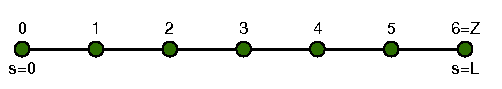
\includegraphics[width=11cm, keepaspectratio=true]{sections/cosserat_rods/images/DiscretizationWeakFormNodes}
    \end{figure}
    with $Z$ elements and $Z+1$ nodes
    
    \vspace{0.7em}
    we discretize the displacements by
    \begin{displaymath}
      \Delta \underline{r}(s) \approx \Delta \underline{r}_i \cdot N_i(s)
    \end{displaymath}
    \begin{displaymath}
      \Delta \underline{\Theta}(s) \approx \Delta \underline{\Theta}_i \cdot N_i(s)
    \end{displaymath}
    
    \vspace{0.5em}
    and the test functions by
    \begin{displaymath}
      \delta \underline{r}(s) \approx \delta \underline{r}_i \cdot N_i(s)
    \end{displaymath}
    \begin{displaymath}
      \delta \underline{\Theta}(s) \approx \delta \underline{\Theta}_i \cdot N_i(s)
    \end{displaymath}
    
    \vspace{1em}
    with shape functions $N_i(s)$ such that
    \begin{displaymath}
      N_i(s) =
      \begin{cases}
        1 & \text{at node } i \\
        0 & \text{at every other node}
      \end{cases}
    \end{displaymath}
    
    \vspace{1em}
    example with linear shape functions:
    \begin{figure}
      \centering
      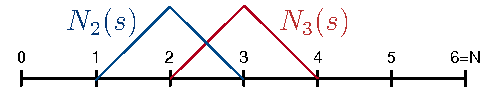
\includegraphics[width=11cm, keepaspectratio=true]{sections/cosserat_rods/images/DiscretizationWeakFormShapeFunction}
    \end{figure}
    
    \vspace{0.5em}
    meaning of $\Delta \underline{r}_i$, $\Delta \underline{\Theta}_i$:
    \begin{displaymath}
      \Delta \underline{r}(s_j) \approx \Delta \underline{r}_i \cdot N_i(s_j) =
      \Delta \underline{r}_i \cdot \delta_{ij} = \underline{r}_j
    \end{displaymath}
    $\rightarrow$ approximated displacements at the nodes
    
    \vspace{0.3em}
    $\rightarrow$ interpolation of displacements via \newline
    \null \quad \:shape functions between the nodes
    
  \end{multicols}
\end{frame}


%-------------------------------------------------------------------------------
\begin{frame}
  \frametitle{Discretization of the weak form (part 2)}

  recall the nonlinear weak form
  \begin{displaymath}
    G_{\text{stat}} = 
      \int_0^L
        \begin{bmatrix}
          \underline{n} \\ \underline{m}
        \end{bmatrix}
        \cdot \doubleunderline{E}^{\mathrm{T}}(s) \cdot
        \begin{bmatrix}
          \delta \underline{r} \\ \delta \underline{\Theta}
        \end{bmatrix}
      \: \dif s \:
      - \int_0^L
        \begin{bmatrix}
          \underline{\hat{n}} \\ \underline{\hat{m}}
        \end{bmatrix} \cdot
        \begin{bmatrix}
          \delta \underline{r} \\ \delta \underline{\Theta}
        \end{bmatrix}
      \: \dif s \:
      - \begin{bmatrix}
          \underline{n}_p \\ \underline{m}_p
      \end{bmatrix} \cdot
      \begin{bmatrix}
          \delta \underline{r} \\ \delta \underline{\Theta}
      \end{bmatrix}
      \sVert[3]_0^L
  \end{displaymath}
  
  \vspace{1em}
  we plug in the discrete approximations of the test functions
  \begin{displaymath}
    \delta \underline{r}(s) \approx \delta \underline{r}_i \cdot N_i(s)
    \quad \text{ and } \quad
    \delta \underline{\Theta}(s) \approx \delta \underline{\Theta}_i \cdot N_i(s)
  \end{displaymath}
  
  \begin{itemize}
    \item $\underline{n}(s)$, $\underline{m}(s)$ depend on the current state $\bigl( \underline{r}, \, \underline{\Theta} \bigr)$
    \item then we work out the next part ...
      \begin{displaymath}
        \doubleunderline{E}^{\mathrm{T}}(s) \cdot
        \begin{bmatrix}
          \delta \underline{r} \\ \delta \underline{\Theta}
        \end{bmatrix} =
        \begin{bmatrix}
          \doubleunderline{I} \, \od{}{s} & [ \underline{r}^{\prime}(s) ]_{\times} \\
          \doubleunderline{0}             & \doubleunderline{I} \, \od{}{s}
        \end{bmatrix} \cdot
        \begin{bmatrix}
          \delta \underline{r} \\ \delta \underline{\Theta}
        \end{bmatrix} =
        \begin{bmatrix}
          \delta \underline{r}^{\prime} + \underline{r}^{\prime} \times \delta \underline{\Theta} \\
          \delta \underline{\Theta}^{\prime}
        \end{bmatrix} \approx
      \end{displaymath}
      \begin{displaymath}
        \approx
        \begin{bmatrix}
          \delta \underline{r}_i \cdot N_i^{\prime}(s) + \underline{r}^{\prime} \times \left( N_i(s) \cdot \delta \underline{\Theta}_i \right) \\
          \delta \underline{\Theta}_i \cdot N_i^{\prime}(s)
        \end{bmatrix} =
        \underbrace{
        \begin{bmatrix}
          N_i^{\prime}(s) \, \doubleunderline{I}  & N_i(s) \, [\underline{r}^{\prime}(s)]_{\times} \\
          \doubleunderline{0}                     & N_i^{\prime} \, \doubleunderline{I}
        \end{bmatrix} }_{=: \doubleunderline{E}_i^{\mathrm{T}}(s)} \cdot
        \begin{bmatrix}
          \delta \underline{r}_i \\
          \delta \underline{\Theta}_i
        \end{bmatrix}
      \end{displaymath}
    note that $\doubleunderline{E}_i^{\mathrm{T}}$ is a regular matrix instead of being an operator written in matrix form
  \end{itemize}
\end{frame}


%-------------------------------------------------------------------------------
\begin{frame}
  \frametitle{Discretization of the weak form (part 3)}
  
  \begin{itemize}
    \item the term for the distributed forces is straightforward: \newline
       we just dot the forces with the approximated test functions
    \item the boundary term can be simplified: e.g. at $s=L$ we have
      \begin{displaymath}
        \delta \underline{r}(L) \approx N_i(L) \cdot \delta \underline{r}_i = N_Z(L) \cdot \delta \underline{r}_Z = \delta \underline{r}_Z
      \end{displaymath}
  \end{itemize}

  we obtain $G_{\text{stat}}^h \bigl( \underline{r}, \, \underline{\Theta} \, ; \, \delta \underline{r}, \, \delta \underline{\Theta} \bigr) =$
  \begin{displaymath}
    \int_0^L
        \begin{bmatrix}
          \underline{n} \\ \underline{m}
        \end{bmatrix}
        \cdot \doubleunderline{E}_i^{\mathrm{T}} \cdot
        \begin{bmatrix}
          \delta \underline{r}_i \\ \delta \underline{\Theta}_i
        \end{bmatrix}
      \: \dif s \:
      - \int_0^L
        \begin{bmatrix}
          \underline{\hat{n}} \\ \underline{\hat{m}}
        \end{bmatrix} \cdot N_i \cdot
        \begin{bmatrix}
          \delta \underline{r}_i \\ \delta \underline{\Theta}_i
        \end{bmatrix}
      \: \dif s \:
      - \begin{bmatrix}
          \underline{n}_p(L) \\ \underline{m}_p(L)
      \end{bmatrix} \cdot
      \begin{bmatrix}
          \delta \underline{r}_Z \\ \delta \underline{\Theta}_Z
      \end{bmatrix}
      + \begin{bmatrix}
          \underline{n}_p(0) \\ \underline{m}_p(0)
      \end{bmatrix} \cdot
      \begin{bmatrix}
          \delta \underline{r}_0 \\ \delta \underline{\Theta}_0
      \end{bmatrix}
  \end{displaymath}
  
  \begin{multicols}{2}
    \noindent
    for a cantilever problem
    \begin{figure}
      \centering
      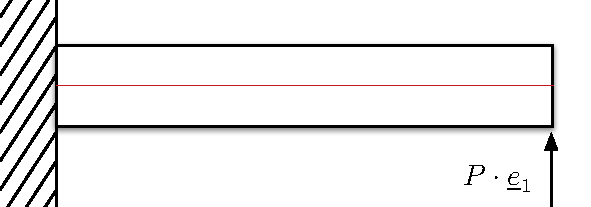
\includegraphics[width=11cm, keepaspectratio=true]{sections/cosserat_rods/images/SimpleCanitleverExample}
    \end{figure}
    
    we have
    \begin{itemize}
      \item $\underline{n}_p(L) = P \cdot \underline{e}_1$ and $\underline{m}_p(L) = 0$
      \item and on the clamped end the boundary term vanishes since $\delta \underline{r}_0 = \delta \underline{\Theta}_0 = 0$ (admissibility)
    \end{itemize} 
  \end{multicols}
  
\end{frame}



%-------------------------------------------------------------------------------
\begin{frame}
  \frametitle{Discretization of the weak form (part 4)}

  we can rewrite the discretized weak form using a global residual vector $\underline{R}$
  \begin{displaymath}
    G_{\text{stat}}^h \bigl( \underline{r}, \, \underline{\Theta} \, ; \, \delta \underline{r}, \, \delta \underline{\Theta} \bigr) =
    \underbrace{
    \begin{bmatrix}
      \begin{bmatrix}
        \underline{R}_0 \\
        \null 
      \end{bmatrix}
      \\ \\
      \begin{bmatrix}
        \underline{R}_1 \\
        \null
      \end{bmatrix}
      \\
      \vdots
      \\
      \begin{bmatrix}
        \underline{R}_Z \\
        \null
      \end{bmatrix}
    \end{bmatrix}
    }_{=: \underline{R}}
    \cdot
    \underbrace{
    \begin{bmatrix}
      \begin{bmatrix}
        \delta \underline{r}_0 \\
        \delta \underline{\Theta}_0
      \end{bmatrix}
      \\ \\
      \begin{bmatrix}
        \delta \underline{r}_1 \\
        \delta \underline{\Theta}_1
      \end{bmatrix}
      \\
      \vdots
      \\
      \begin{bmatrix}
        \delta \underline{r}_Z \\
        \delta \underline{\Theta}_Z
      \end{bmatrix}
    \end{bmatrix}
    }_{=: \underline{\delta}}
  \end{displaymath}
  
  with $Z+1$ blocks / $6$ dimensional subvectors of $\underline{R}$ defined as
  \begin{displaymath}
    \underline{R}_i =
    \int_0^L
      \doubleunderline{E}_i(s) \cdot
      \begin{bmatrix}
        \underline{n}(s) \\ \underline{m}(s)
      \end{bmatrix}
    \: \dif s \:
    - \int_0^L
      N_i(s)
      \begin{bmatrix}
        \underline{\hat{n}}(s) \\ \underline{\hat{m}}(s)
      \end{bmatrix}
    \: \dif s \:
  \end{displaymath}
  
  the boundary terms are added to $\underline{R}_0$ and $\underline{R}_Z$

\end{frame}


%-------------------------------------------------------------------------------
\begin{frame}
  \frametitle{Discretization of the weak form (part 5)}

  \textbf{assembly of the residual vector}

  for each of the $Z+1$ subvectors we integrate from $s=0$ to $s=L$ \newline
  the integration domain can be divided into the $Z$ elements
  \begin{displaymath}
    \underline{R}_i =
    \sum_{e=0}^{Z}
    \Biggl(
    \int_{s_{e-1}}^{s_e}
      \doubleunderline{E}_i(s) \cdot
      \begin{bmatrix}
        \underline{n}(s) \\ \underline{m}(s)
      \end{bmatrix}
    \: \dif s \:
    - \int_{s_{e-1}}^{s_e}
      N_i(s)
      \begin{bmatrix}
        \underline{\hat{n}}(s) \\ \underline{\hat{m}}(s)
      \end{bmatrix}
    \: \dif s \:
    \Biggr)
  \end{displaymath}

  now we can exploit the compactness of the shape functions
  
  \vspace{1em}
  $\Delta \underline{r}(s) \approx \Delta \underline{r}_i \cdot N_i(s)$, 
  $\Delta \underline{\Theta}(s) \approx \Delta \underline{\Theta}_i \cdot N_i(s)$
\end{frame}